\chapter{Chapter 3. Data and Methodology}

\section{Dataset Overview}

This section includes a description of the storage of and framework used to interface with the data, insights on the value distributions and spatial variability of the input forcings from NLDAS-2, as well as a look at similar bulk properties of the target soil moisture states and governing processes within Noah-LSM. In this work, we define our valid domain to include all points falling within the conterminous United States, excluding those points within the NLDAS-2 domain falling with Canada and Mexico. We also exclude points that are classified as ``water,'' ``bedrock,'' or ``other'' in the STATSGO dataset, since they don't correspond to meaningful hydraulic properties, and have idle time series. What remains are 50,875 candidate grid cells within a 224x464 pixel domain.

\subsection{Data Storage System}

The data used in this project were acquired from the Goddard Earth Sciences Data and Information Services Center's Distributed Active Archive Center (GES DISC DAAC) in May of 2024. The DAAC archives the NLDAS-2 forcings and corresponding Noah-LSM model outputs as separate hourly files in a GRIB1 format, of which we downloaded the full 12-year time series from January 1, 2012 to December 31, 2023. This subset constitutes 210,384 files with a total size of just over 891.38 GB.

Since this project concerns developing 2-week time series of the forcings on a per-pixel basis, it would be inefficient to extract data from several hundred files for each sequence sample. Furthermore, it is widely recognized in deep learning that input/target pairs from heterogeneous datasets should be globally shuffled during the training process, as outlined by \citep{nguyen_why_2022}. This is because local subsets may have distribution characteristics that are distinct from the full dataset, so as the model trains on an unshuffled dataset, the loss gradients it experiences may encourage it to converge on a locally-optimal solution that does not generalize well to the overall task. Shuffling is especially salient for geoscience datasets like this one, which are highly spatially and temporally heterogeneous. With this in mind, the overhead from file I/O operations would be prohibitive for sporadically drawing samples from throughout the GRIB dataset during training or inference.

To address this problem while maintaining the spatiotemporal structure of the data, we develop a custom file standard using the HDF5 format -- hereafter referred to as the \textsc{timegrid} -- and extract the full 12-year NLDAS and Noah-LSM record as a collection of them. The HDF5 format offers a system for memory-mapped data chunking in multiple dimensions, which means the data therein can be sparsely buffered and accessed on a per-chunk basis without loading the entire file into memory: a considerable advantage for thoroughly shuffling or accessing subsets of contiguous data within large files. In practice, each timegrid contains 3 years of data covering 1/6 of the spatial domain, and stores the 4-dimensional time-varying data (time, latitude, longitude, data type), 3-dimensional static data (latitude, longitude, data type), and timestamps alongside a string-serialized attribute dictionary. The attributes contain information on abbreviated and full data type names, ordering, units, and sources, which are sufficient to inform a variety of accessor methods with a wealth of downstream use cases.

\subsection{Regional Variance of Input Data}

\begin{figure}[h!]
    \centering
    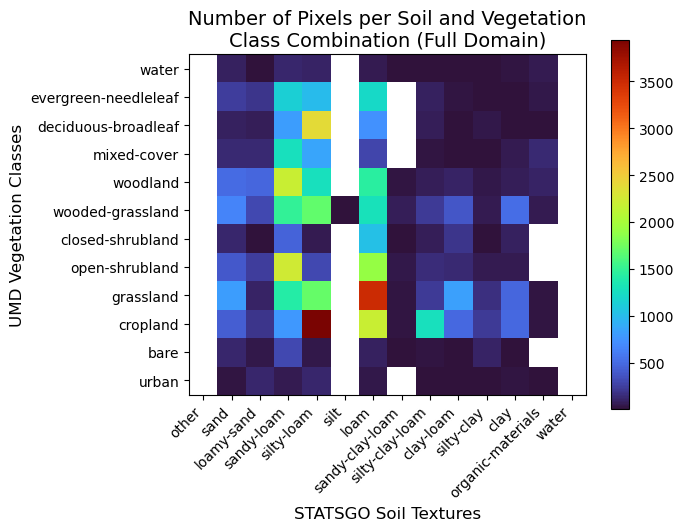
\includegraphics[width=.75\linewidth,draft=false]{figures/static_soil-veg-combos.png}
    \caption{Full-domain combination matrix of vegetation and soil classes}
    \label{static-combos}
\end{figure}

\begin{figure}[hp!]
    \centering
    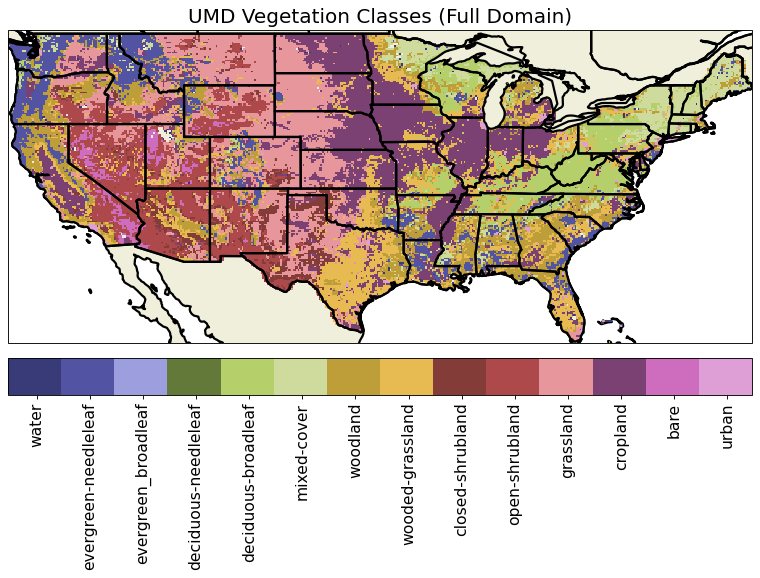
\includegraphics[width=.85\linewidth,draft=false]{figures/static_umd-veg-classes.png}
    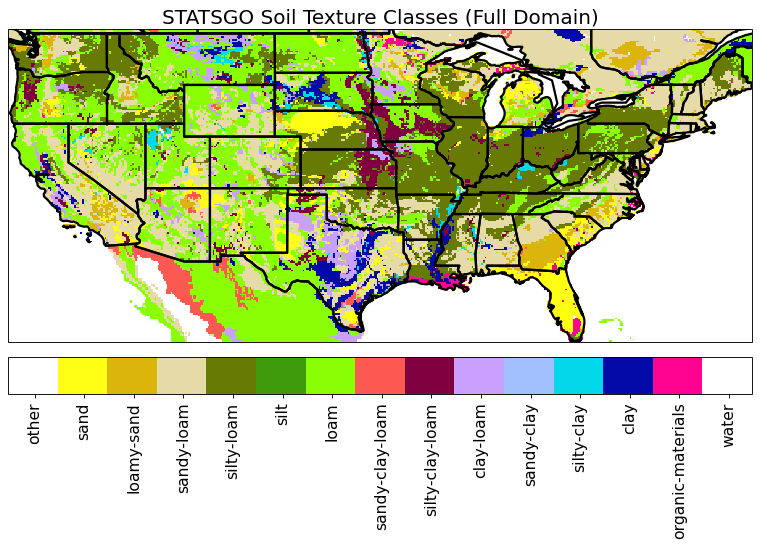
\includegraphics[width=.85\linewidth,draft=false]{figures/static_statsgo-soil-classes.png}
    \caption{Spatial distribution of vegetation and soil classes}
    \label{static-classes}
\end{figure}

\begin{figure}[hp!]
    \centering
    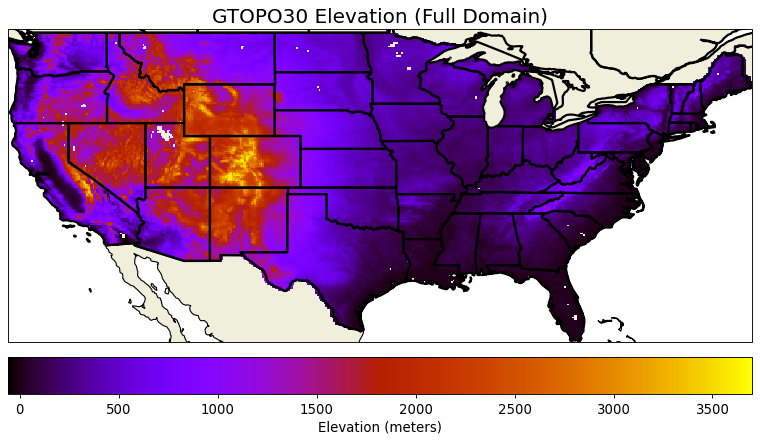
\includegraphics[width=.85\linewidth,draft=false]{figures/static_elev.png}
    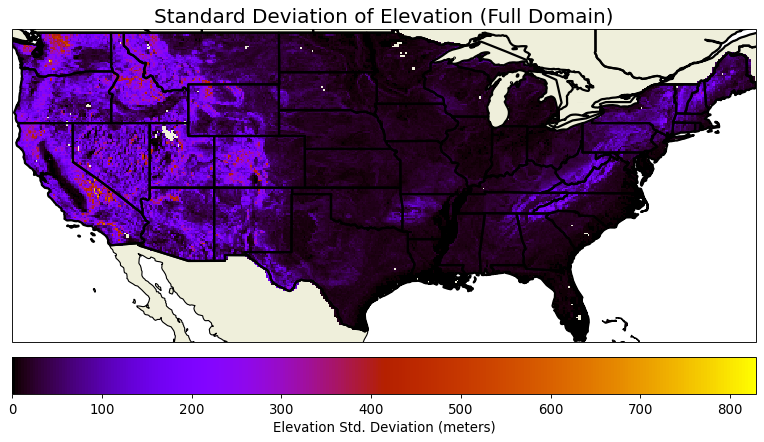
\includegraphics[width=.85\linewidth,draft=false]{figures/static_elev-stdev.png}
    \caption{Elevation and standard deviation of elevation on the CONUS domain}
    \label{static-elevation}
\end{figure}

One important aspect of the NLDAS-2/Noah-LSM datasets is the relationship between static and dynamic parameters, and the regional variance of both of these input types. Given any particular forcing time series, the subsequent land surface response is modulated by values for vegetation type, soil texture, elevation, standard deviation of elevation, slope, and slope aspect, which are consistent per-pixel throughout the dataset. In this work, we will only train models informed by the first four. Slope and aspect were left out because within Noah-LSM they are only used within the snowpack parameterization \citep{barlage_noah_2010}, and snow is generally not a target variables for the models presented here. Furthermore, slope correlates strongly with the standard deviation of elevation. In retrospect, however, these inputs may have increased the information available to the models for estimating the transference of water from snow melt to the soil layers, especially in mountainous regions like the Rocky Mountain and Sierra Nevada ranges. An evaluation of the impact of these parameters on model results is left for future work. Elevation is mainly used to perform orographic regressions on pressure, temperature, humidity, and precipitation while resampling forcing data, however it could be useful as a predictor that indicates processes relevant to mountain snowpack dynamics.

As described in the background, the vegetation classes encode the properties of the canopy relevant to precipitation interception and land surface shading, the efficiency of plant transpiration at removing water from the soil, and the number of layers from which water is drawn (that is, the rooting depth). Since the vegetation parameter is discretely categorical within the Noah-LSM algorithm, we employ a special method of introducing them into the model called class embedding, which is elaborated upon in the next subsection.  The soil texture class corresponds to a variety of hydraulic properties identified by \citep{cosby_statistical_1984}, which include field capacity, hydraulic conductivity, porosity, wilting point, matric potential, and Skempton's pore water pressure (``B'' parameter). These describe physical characteristics of the soil-water system including the rate of downward percolation of water, the efficiency and limits of plant water uptake, the speed of infiltration, and the total amount of water that soil can contain per unit volume. The basic observable feature of soil that determines all of the hydraulic properties is the size distribution of its constituent particles, which is often articulated as the mass fraction of sand, silt, and clay components within the soil. In the interest of providing the models with real-valued inputs having relatively low dimensionality, these three texture components will serve as the representation of soil texture for the ANNs trained here.

The interplay between plant water uptake and soil water dynamics as governed by the static inputs represents a considerable source of complexity within Noah-LSM. Furthermore, as Figure \ref{static-combos} demonstrates, the distribution of combinations of soil and vegetation categories is extremely non-uniform, which makes it more difficult for ANNs to learn solutions that are general. Figure \ref{static-classes} shows the geographic locations of vegetation and soil classes. The most common class combination is silty-loam soil types juxtaposed with cropland, with 3,945 members found dominantly in the Midwest and lower Mississippi river basin, with some contribution from the Columbia Plateau in Washington and Eastern Nebraska. Next most common are the 3,490 pixels in loamy grasslands, which are distributed widely throughout the West US including the high plains, Western Texas and New Mexico,  Utah, and Idaho. The remaining combinations all have fewer than 2,500 members within the domain. Sand and clay dominated soils form the upper and lower extremes of soil particle size, respectively, and thus have rather different soil water characteristics. The sandiest soils are found in Southern Coastal Plains, Michigan, Texas, the Nebraska Sandhills, and the desert Southwest. Clay soils are relatively rare compared to silty and sandy soils, and considerably more spatially heterogeneous. They are mainly found in tight groupings around Central Texas, the Mississippi Alluvial Plain, Eerie Lake Plains, and the Missouri River Basin in South Dakota. Despite their infrequency, clay soils span the full range of surface classes.

\begin{figure}[h!]
    \centering
    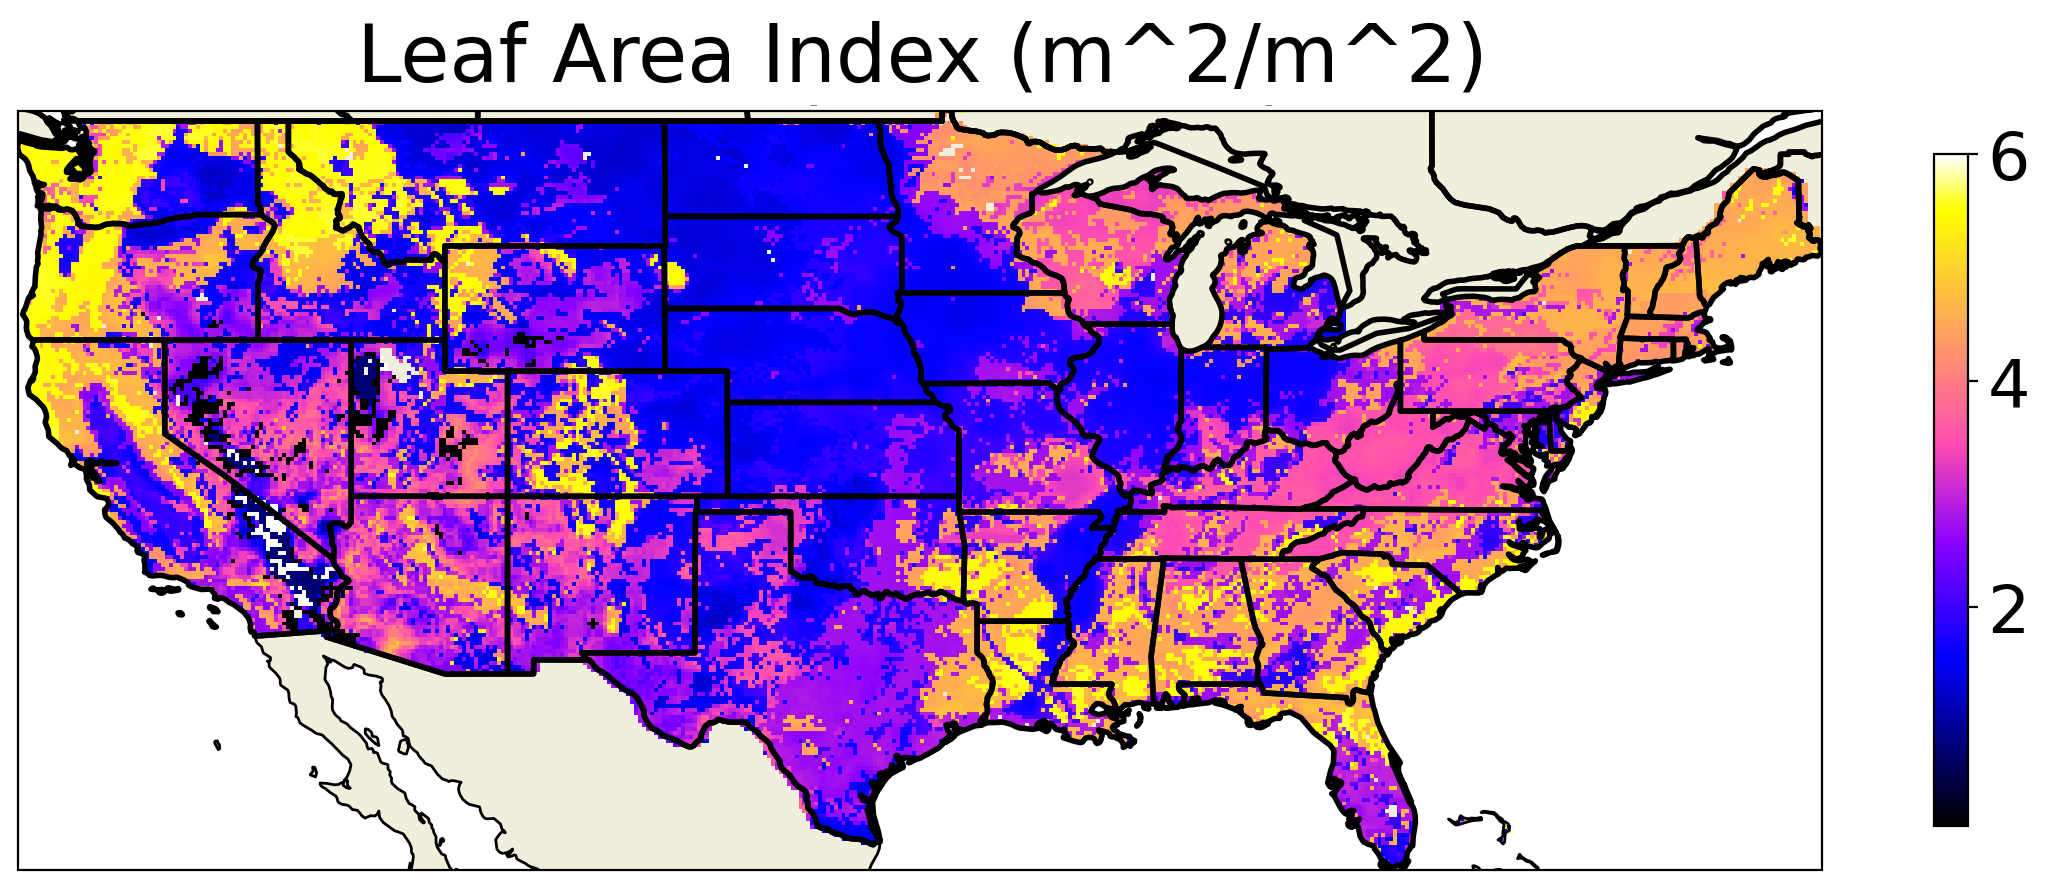
\includegraphics[width=.48\linewidth,draft=false]{figures/thesis-gridstats/gridstat-bulk_lai_2012-1_2023-12_y000-195_x000-462_mean.png}

    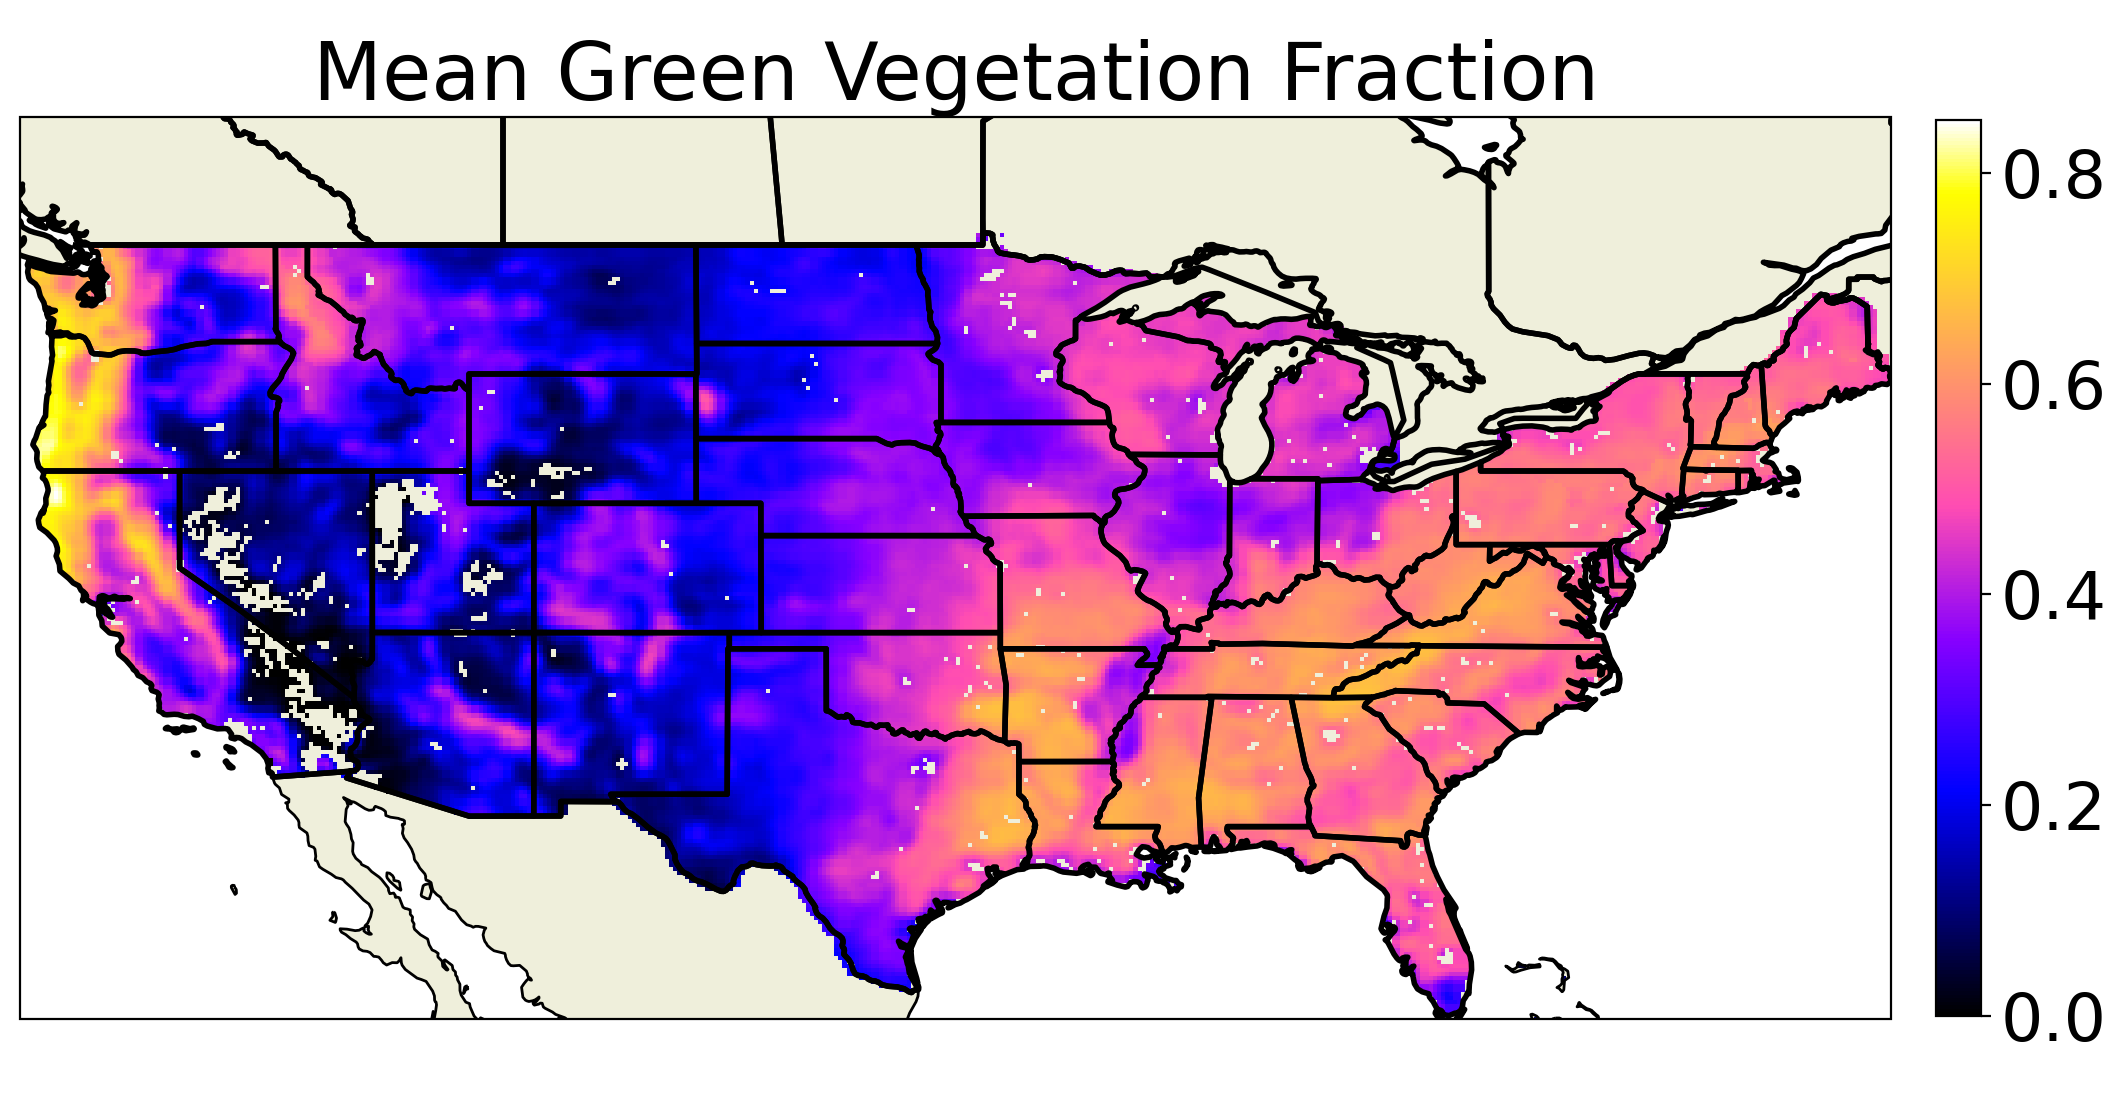
\includegraphics[width=.48\linewidth,draft=false]{figures/thesis-gridstats/gridstat-bulk_veg_2012-1_2023-12_y000-195_x000-462_mean.png}
    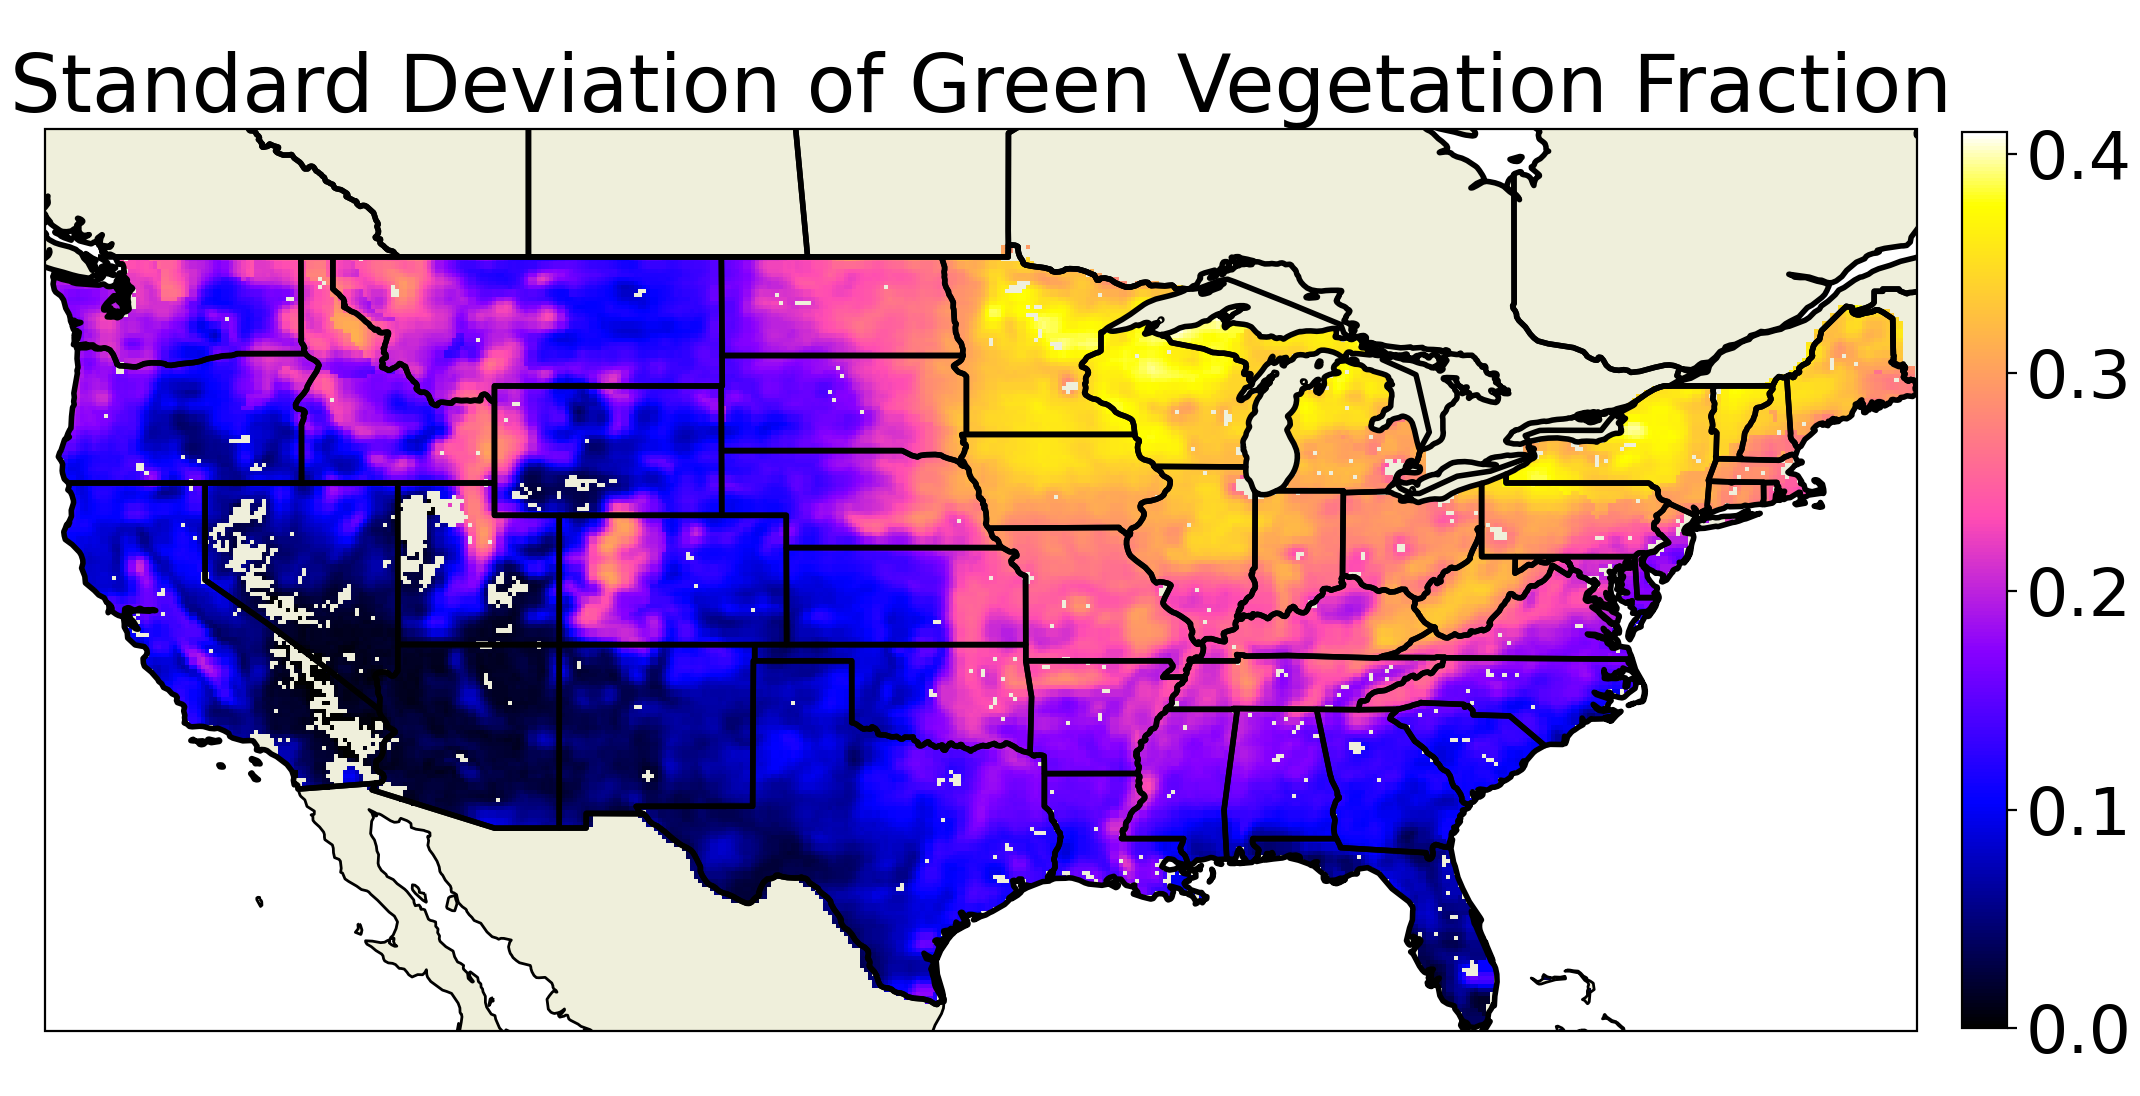
\includegraphics[width=.48\linewidth,draft=false]{figures/thesis-gridstats/gridstat-bulk_veg_2012-1_2023-12_y000-195_x000-462_stdev.png}
    \caption{Gridded mean and standard deviation of vegetation input parameters (2012-2023)}
    \label{gs-vegetation}
\end{figure}

Although they vary smoothly on an hourly basis, the LAI and GVF parameters are similar to static parameters in that they cycle consistently per-pixel on an annual basis (rather than dynamically changing based on variable atmospheric conditions), and modulate the soil water dynamics via through their effect on the vegetation parameterization. As Figure \ref{gs-vegetation} indicates, the densest annual-averaged canopy cover corresponds to evergreen needleleaf surface types, and there is almost no canopy over croplands and grasslands of the Midwest, California Valley, and the Great Plains. The greenest satellite-derived vegetation covers the West Coast and Sierra ranges, followed by the South and Northeast. The standard deviation of GVF indicates the regions of most significant seasonal variability, which corresponds to deciduous-dominant locales.

\begin{figure}[h!]
    \centering
    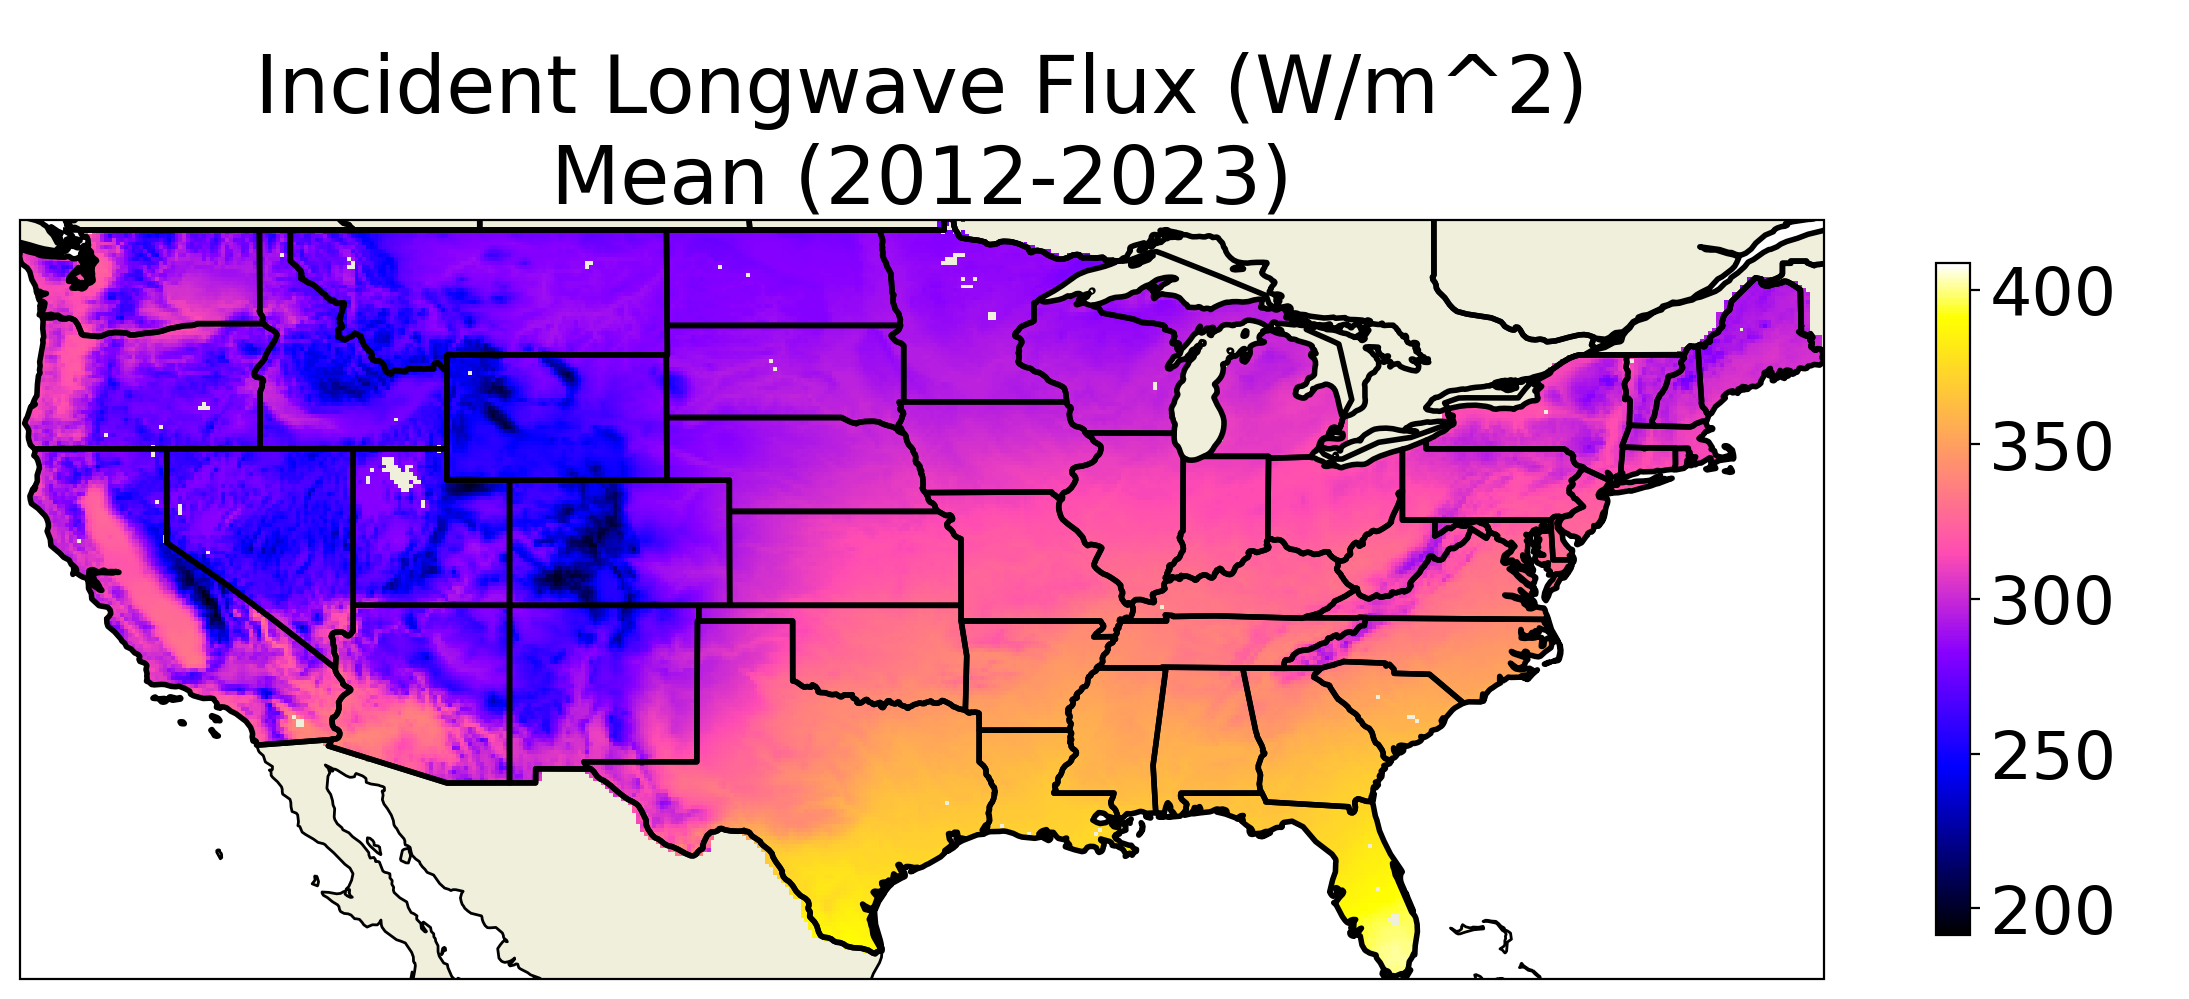
\includegraphics[width=.48\linewidth,draft=false]{figures/thesis-gridstats/gridstat-bulk_dlwrf_2012-1_2023-12_y000-195_x000-462_mean.png}
    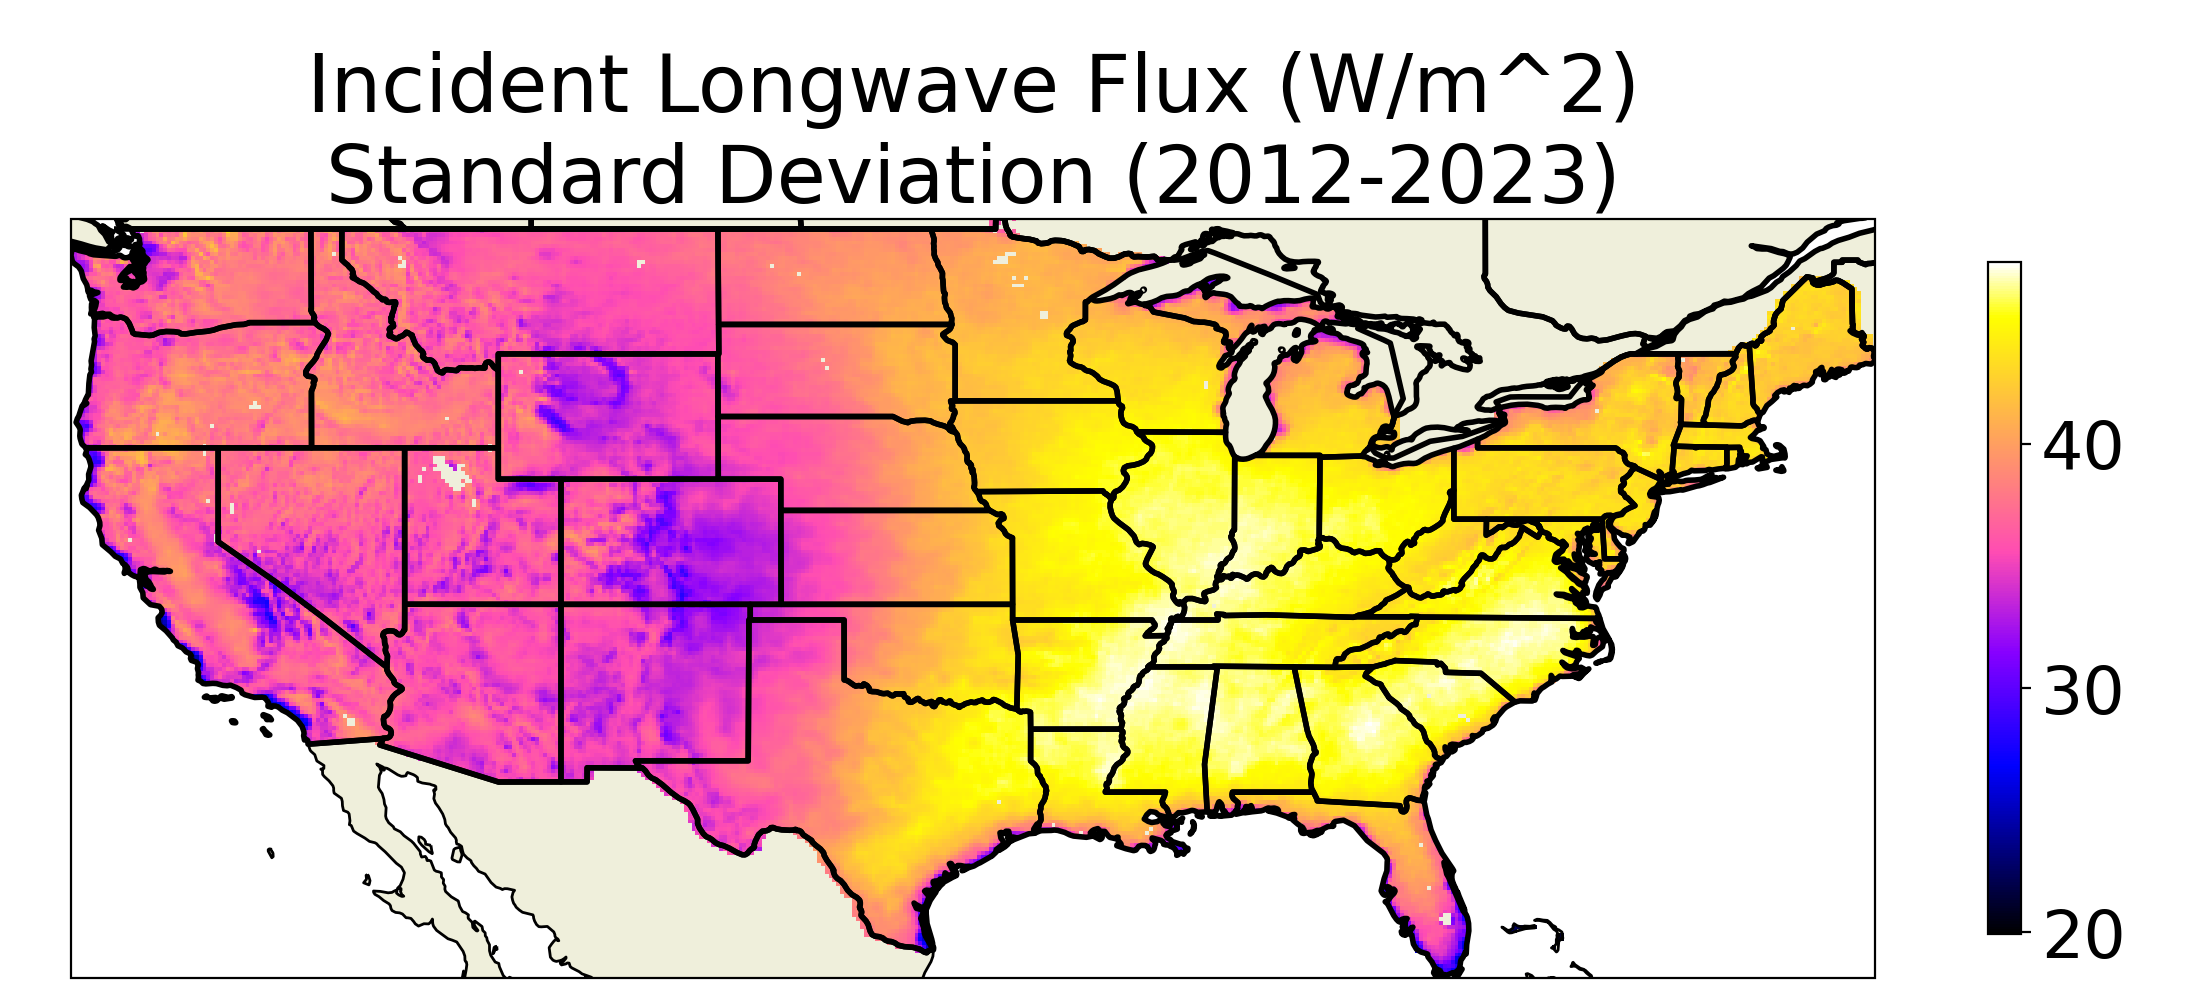
\includegraphics[width=.48\linewidth,draft=false]{figures/thesis-gridstats/gridstat-bulk_dlwrf_2012-1_2023-12_y000-195_x000-462_stdev.png}

    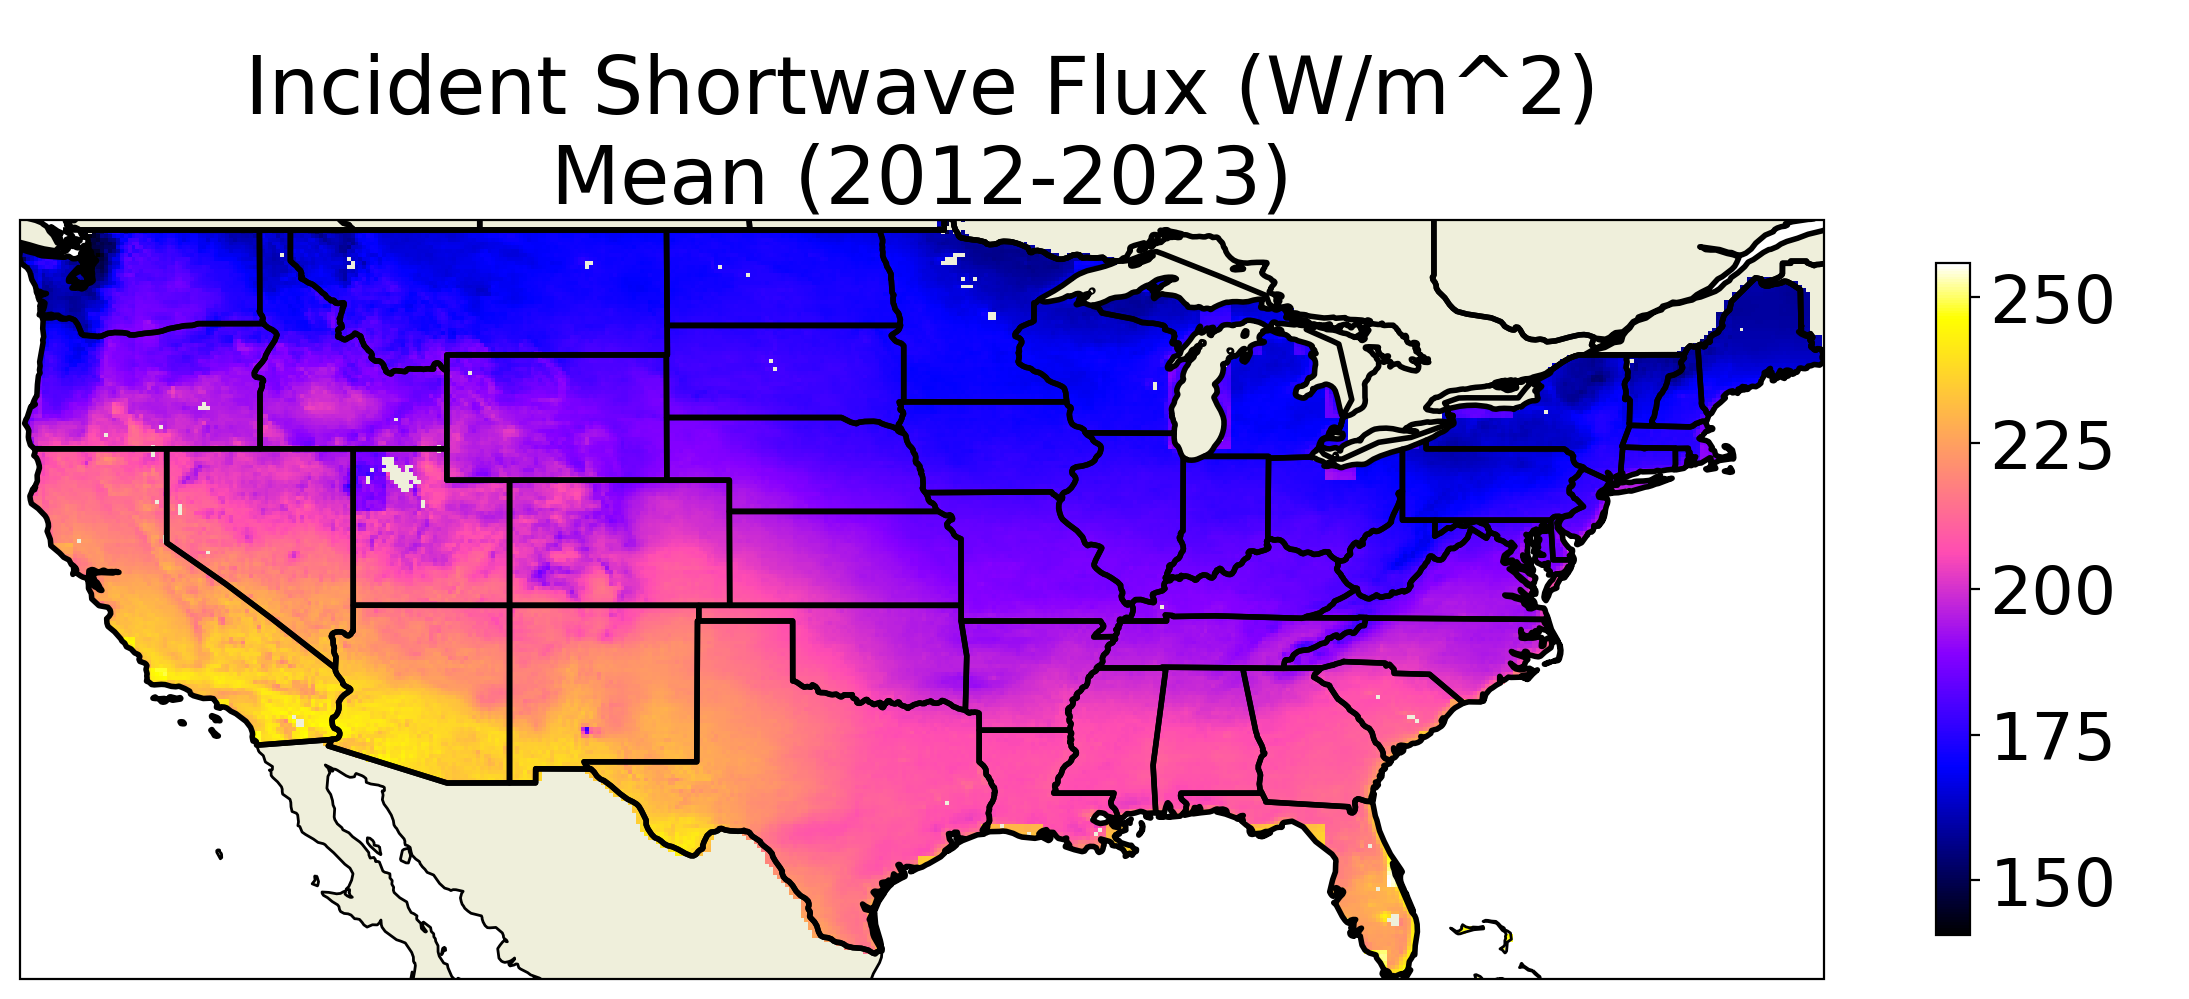
\includegraphics[width=.48\linewidth,draft=false]{figures/thesis-gridstats/gridstat-bulk_dswrf_2012-1_2023-12_y000-195_x000-462_mean.png}
    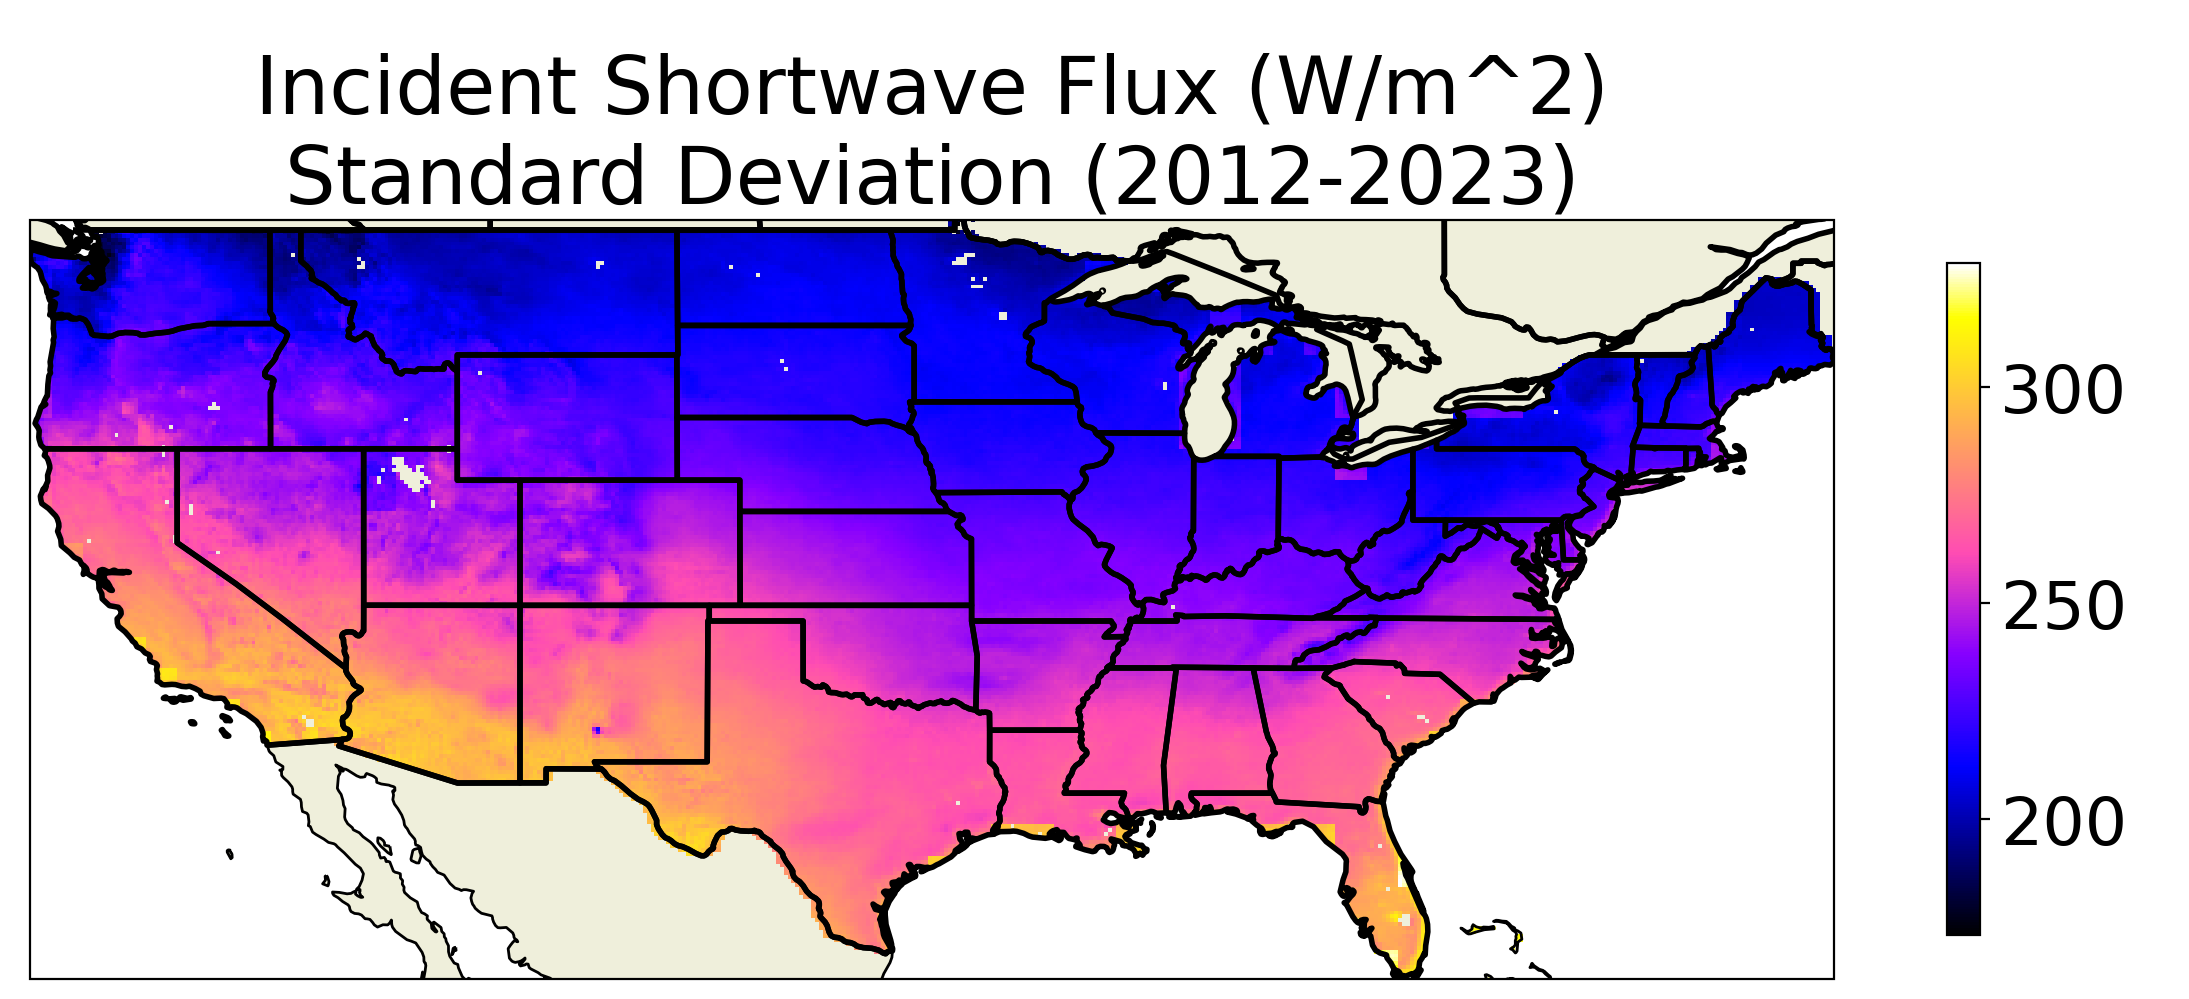
\includegraphics[width=.48\linewidth,draft=false]{figures/thesis-gridstats/gridstat-bulk_dswrf_2012-1_2023-12_y000-195_x000-462_stdev.png}
    \caption{Gridded mean and standard deviation of radiative forcings (2012-2023)}
    \label{gs-radiative}
\end{figure}

In addition to the substantial regional variability of the static parameterization of Noah-LSM, there are considerable regional and seasonal differences in the NLDAS-2 atmospheric forcing time series. Figure \ref{gs-radiative} shows the mean and standard deviation of radiative features over the full spatial and temporal domain, which demonstrates the distribution of annually-averaged downwelling radiation. Feedback from terrestrial emissions mean that longwave radiation is highest in regions that are generally cloudier, have warmer land surface temperatures, and are lower in elevation. The shortwave flux is highest at lower latitudes due to Earth's axial tilt, and in arid regions where there are fewer clouds.

\begin{figure}[hp!]
    \centering
    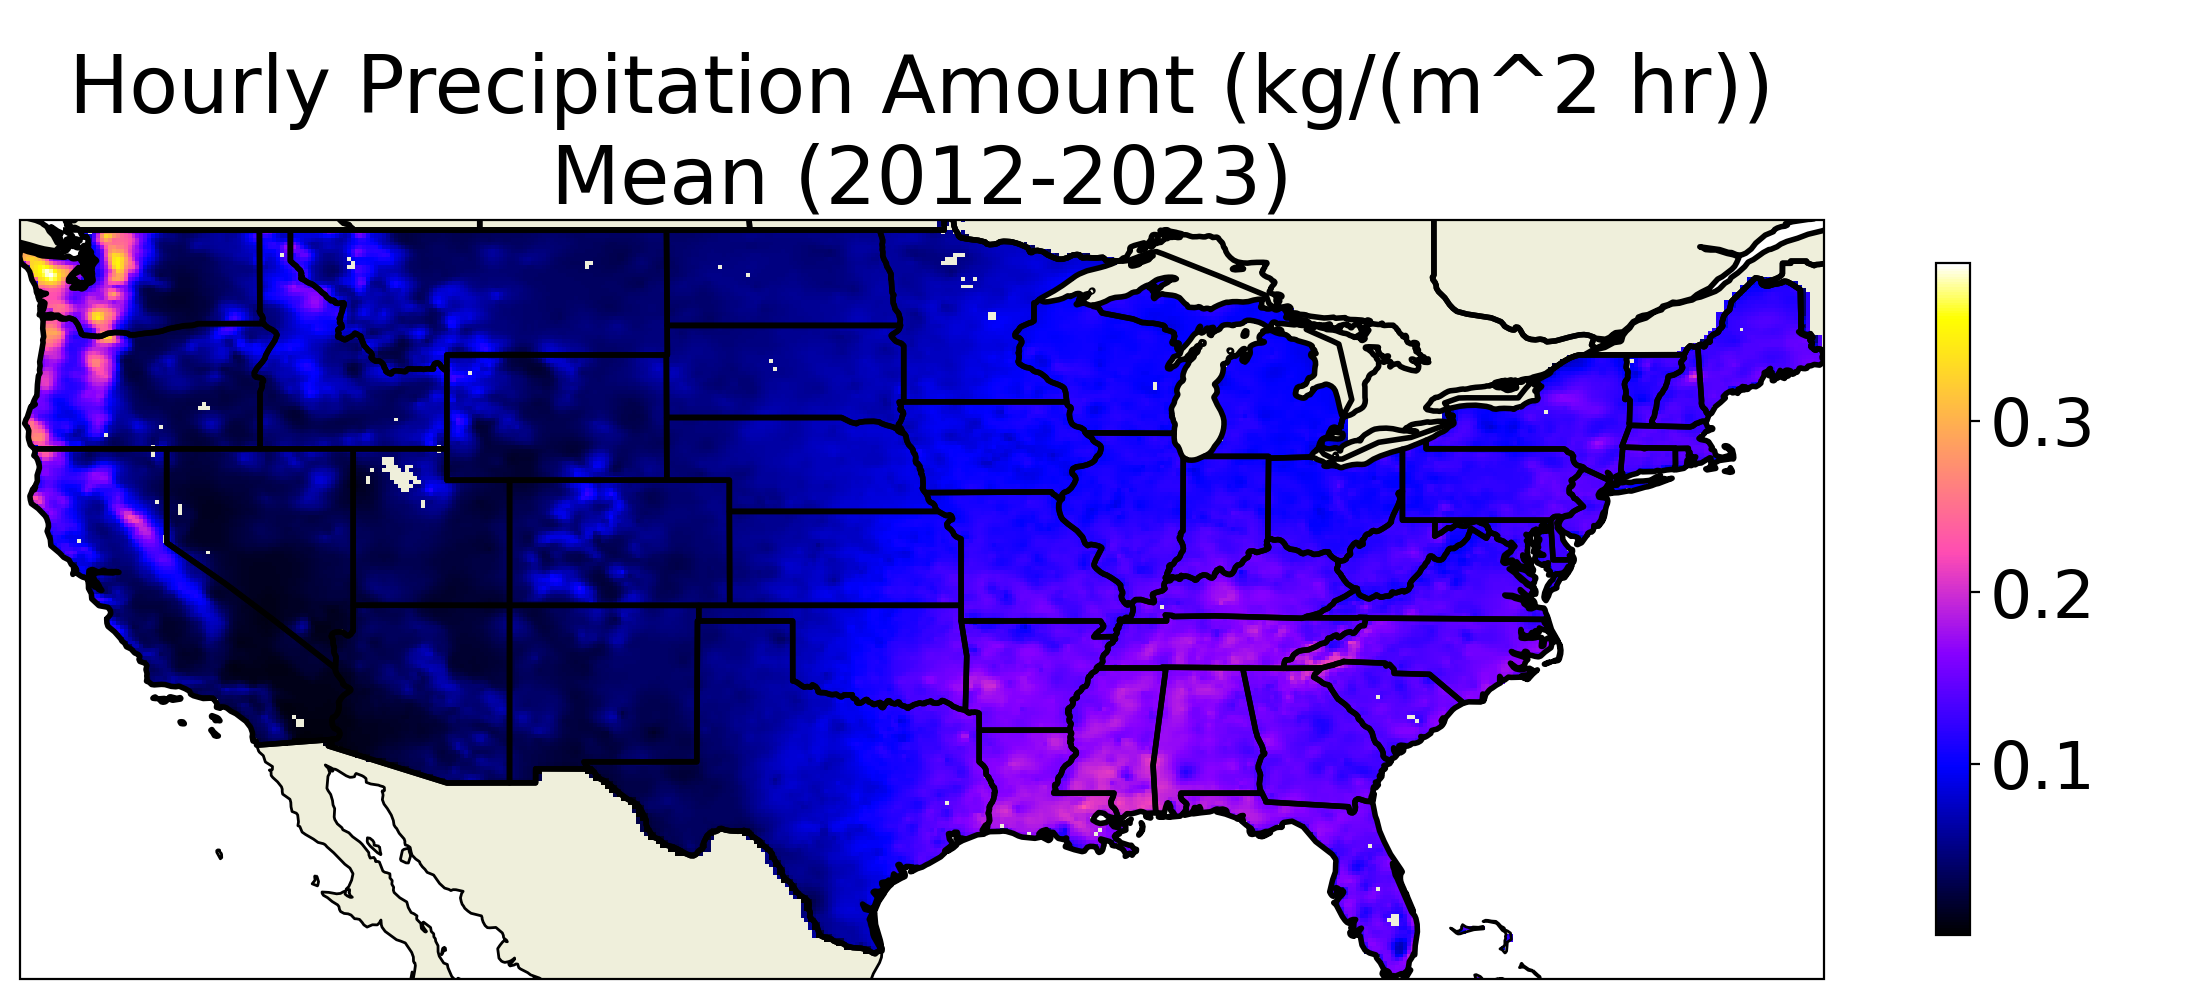
\includegraphics[width=.48\linewidth]{figures/thesis-gridstats/gridstat-bulk_apcp_2012-1_2023-12_y000-195_x000-462_mean.png}
    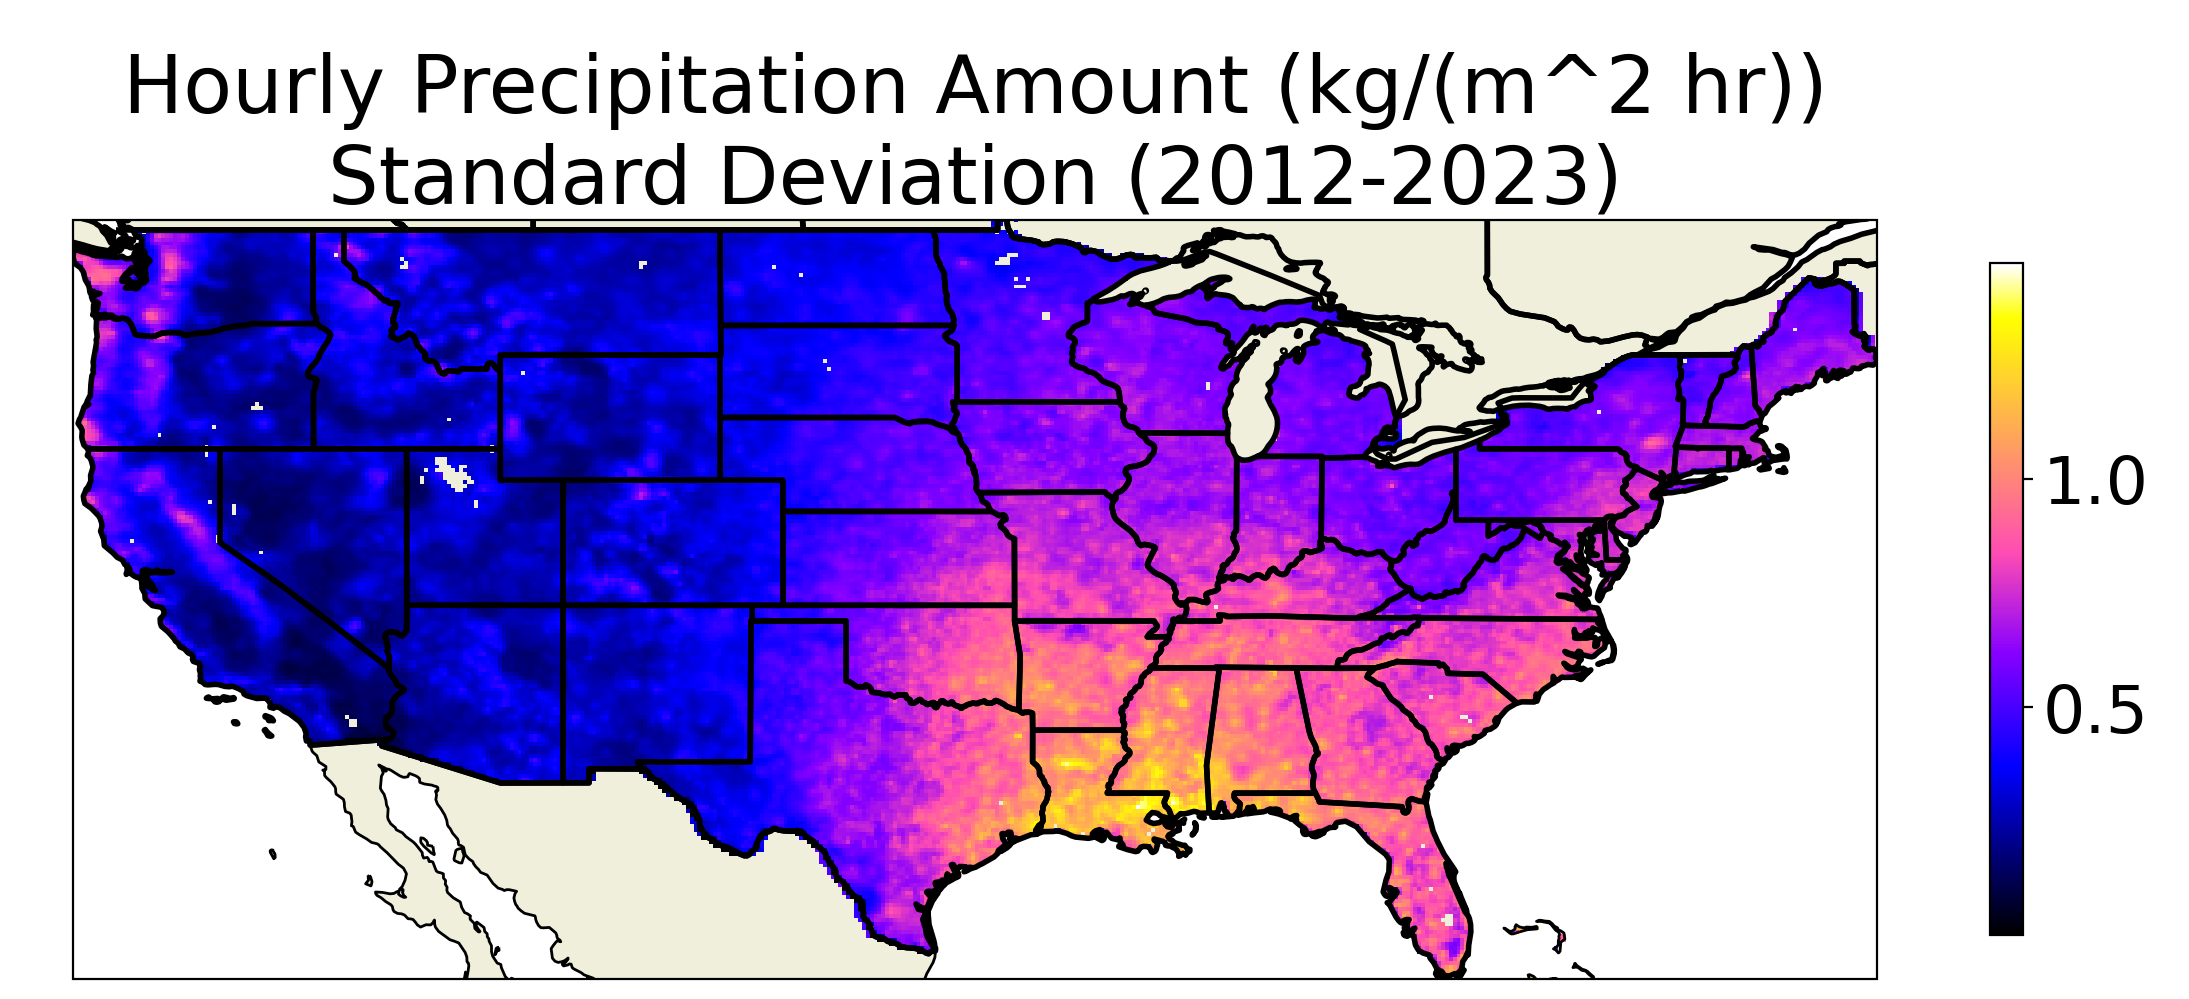
\includegraphics[width=.48\linewidth]{figures/thesis-gridstats/gridstat-bulk_apcp_2012-1_2023-12_y000-195_x000-462_stdev.png}

    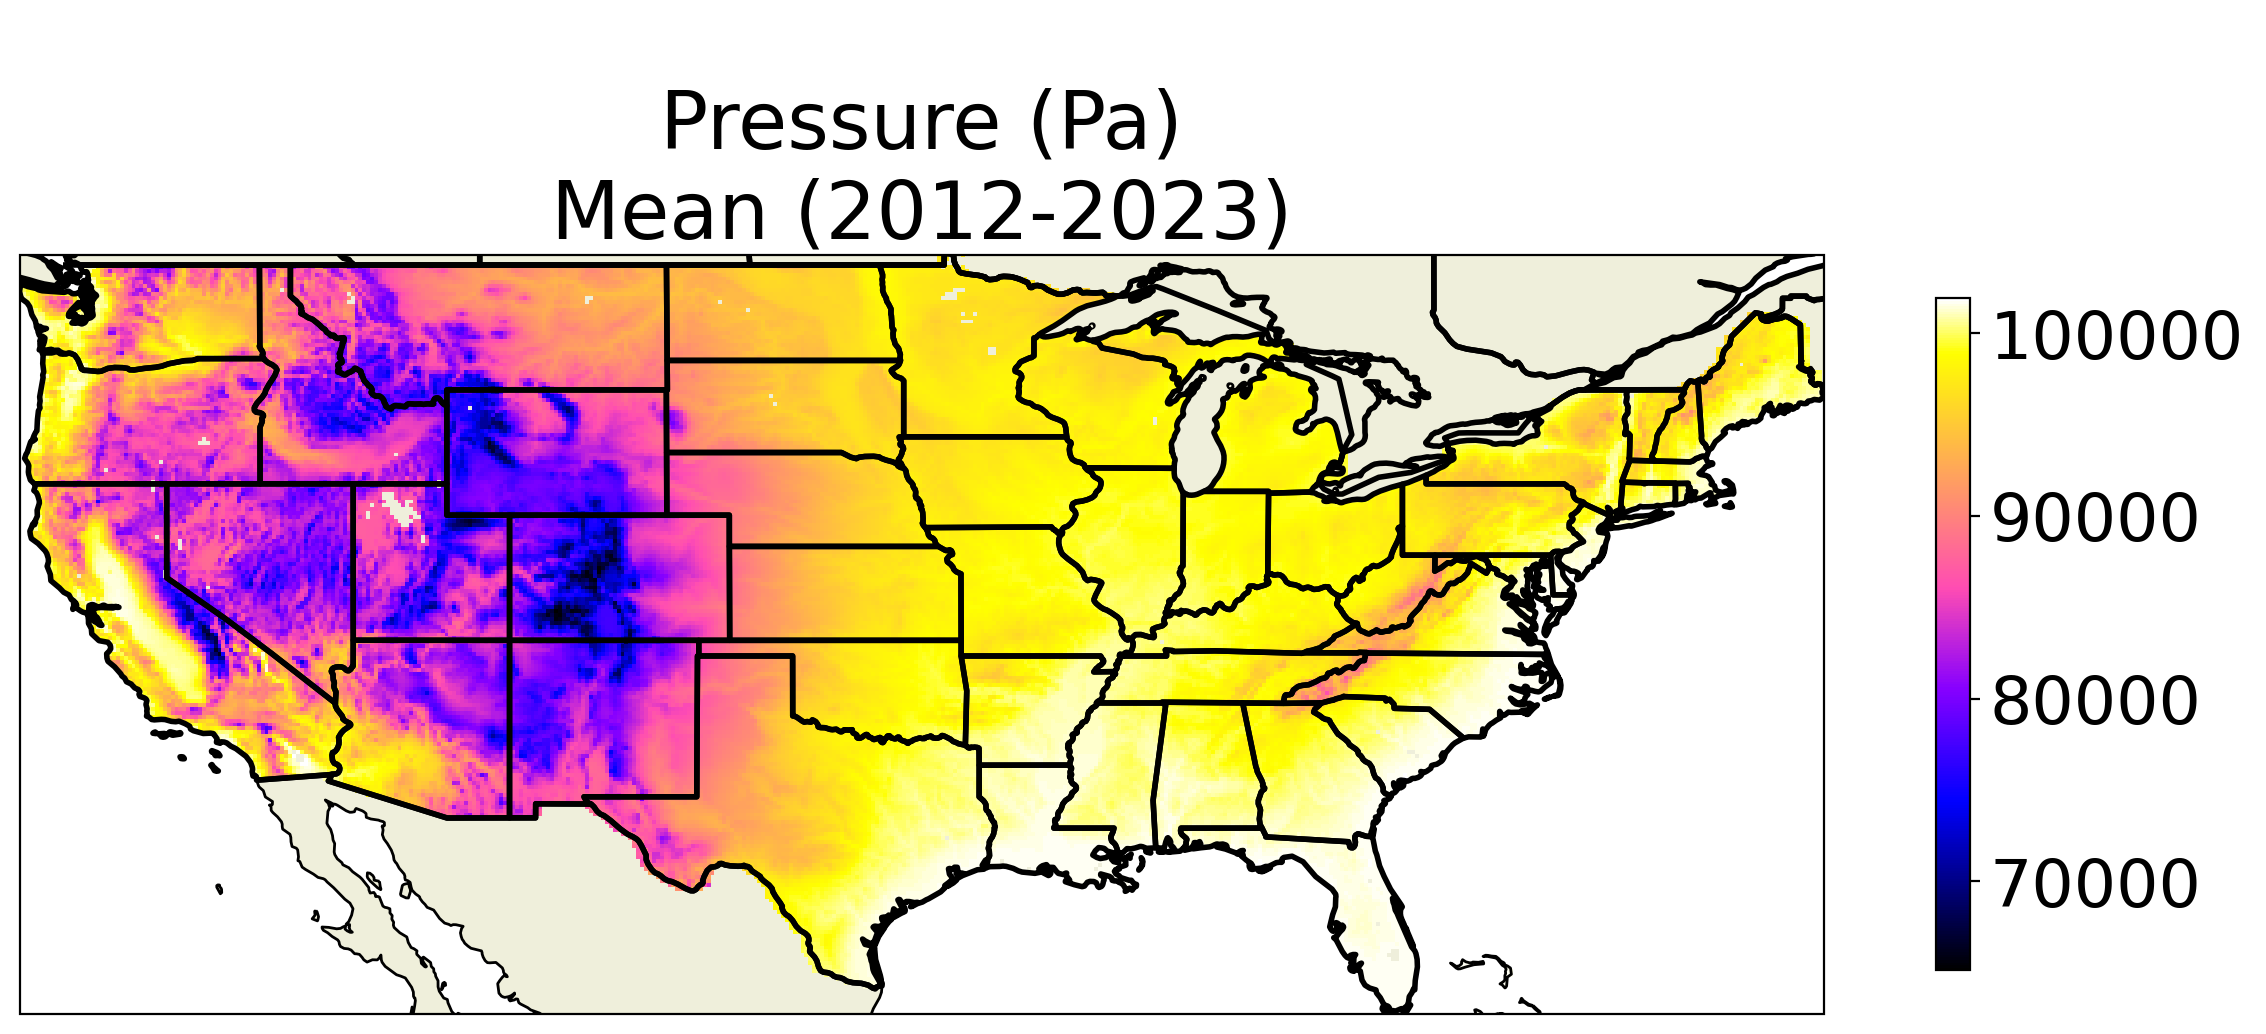
\includegraphics[width=.48\linewidth]{figures/thesis-gridstats/gridstat-bulk_pres_2012-1_2023-12_y000-195_x000-462_mean.png}
    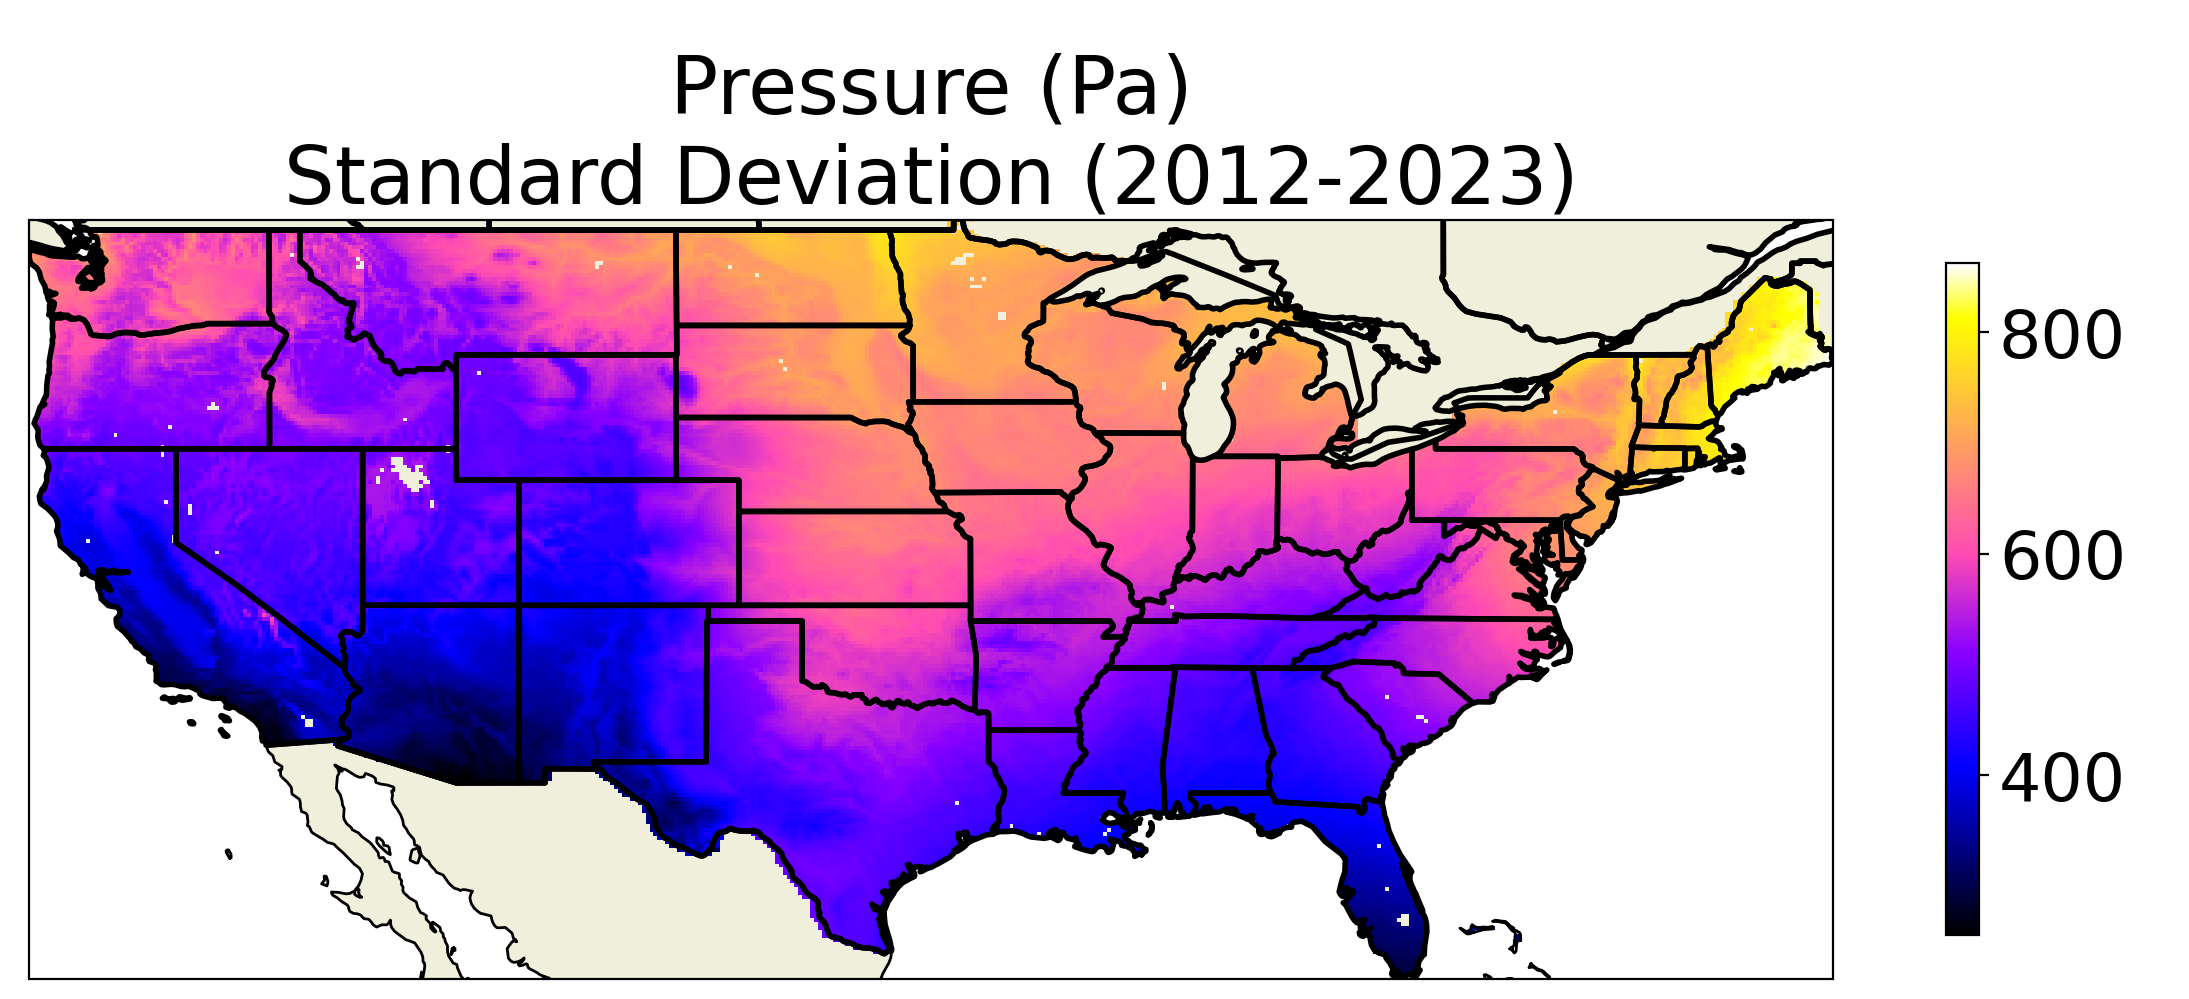
\includegraphics[width=.48\linewidth]{figures/thesis-gridstats/gridstat-bulk_pres_2012-1_2023-12_y000-195_x000-462_stdev.png}

    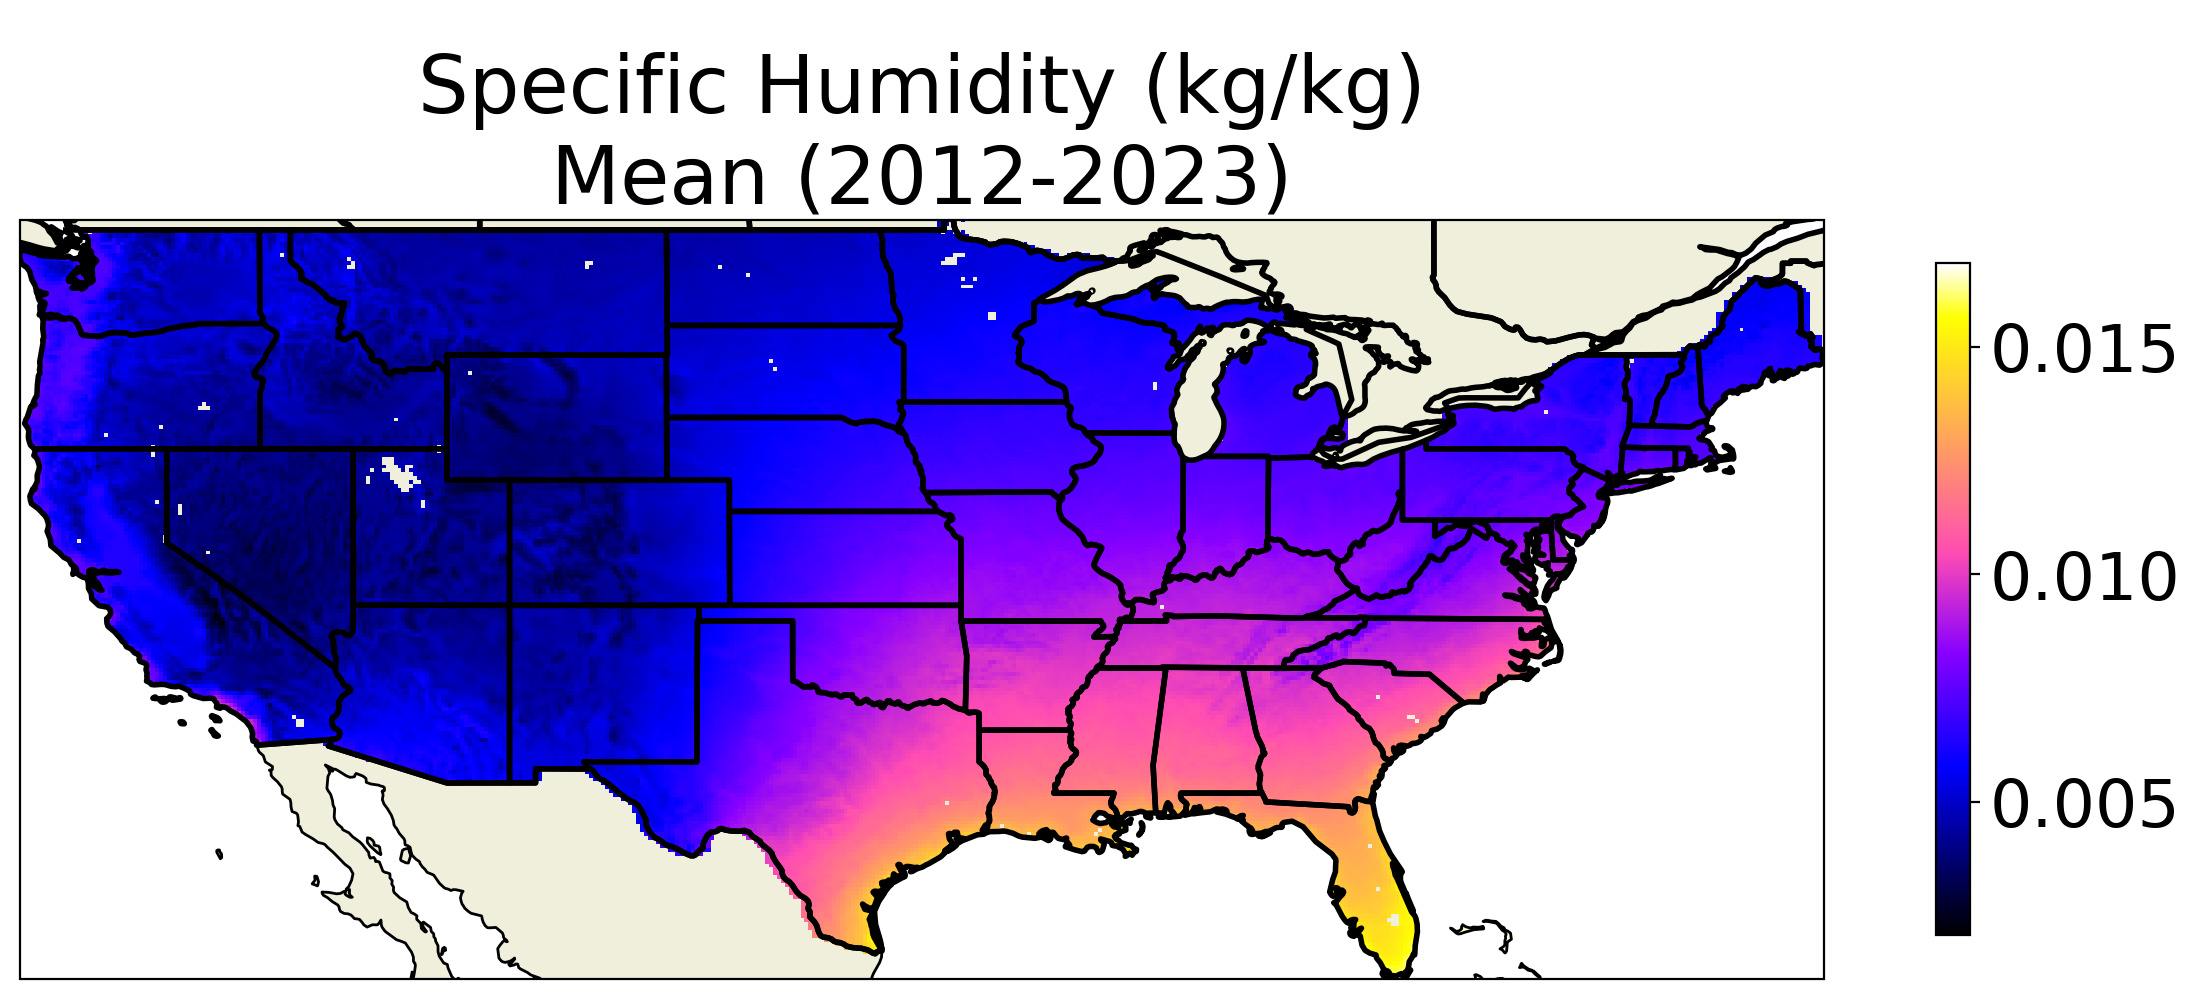
\includegraphics[width=.48\linewidth]{figures/thesis-gridstats/gridstat-bulk_spfh_2012-1_2023-12_y000-195_x000-462_mean.png}
    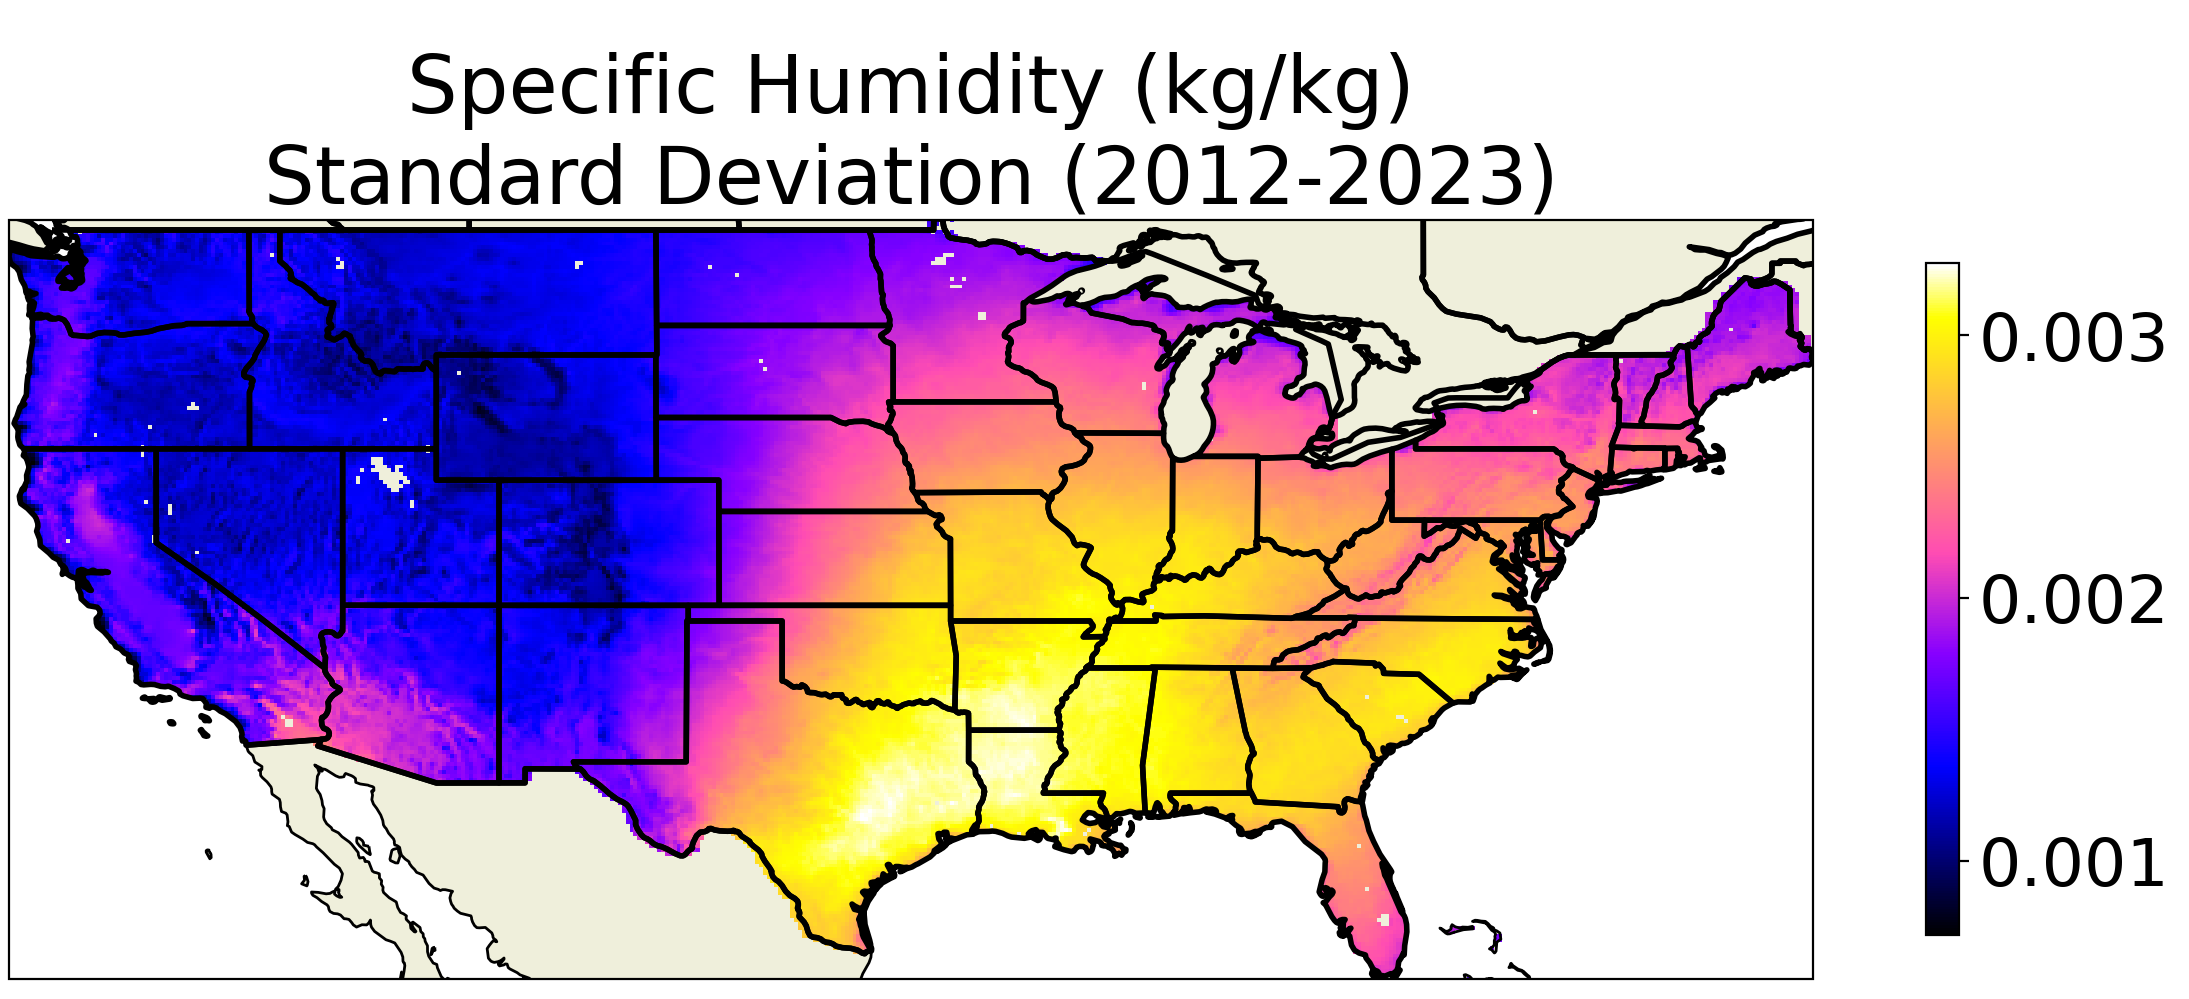
\includegraphics[width=.48\linewidth]{figures/thesis-gridstats/gridstat-bulk_spfh_2012-1_2023-12_y000-195_x000-462_stdev.png}

    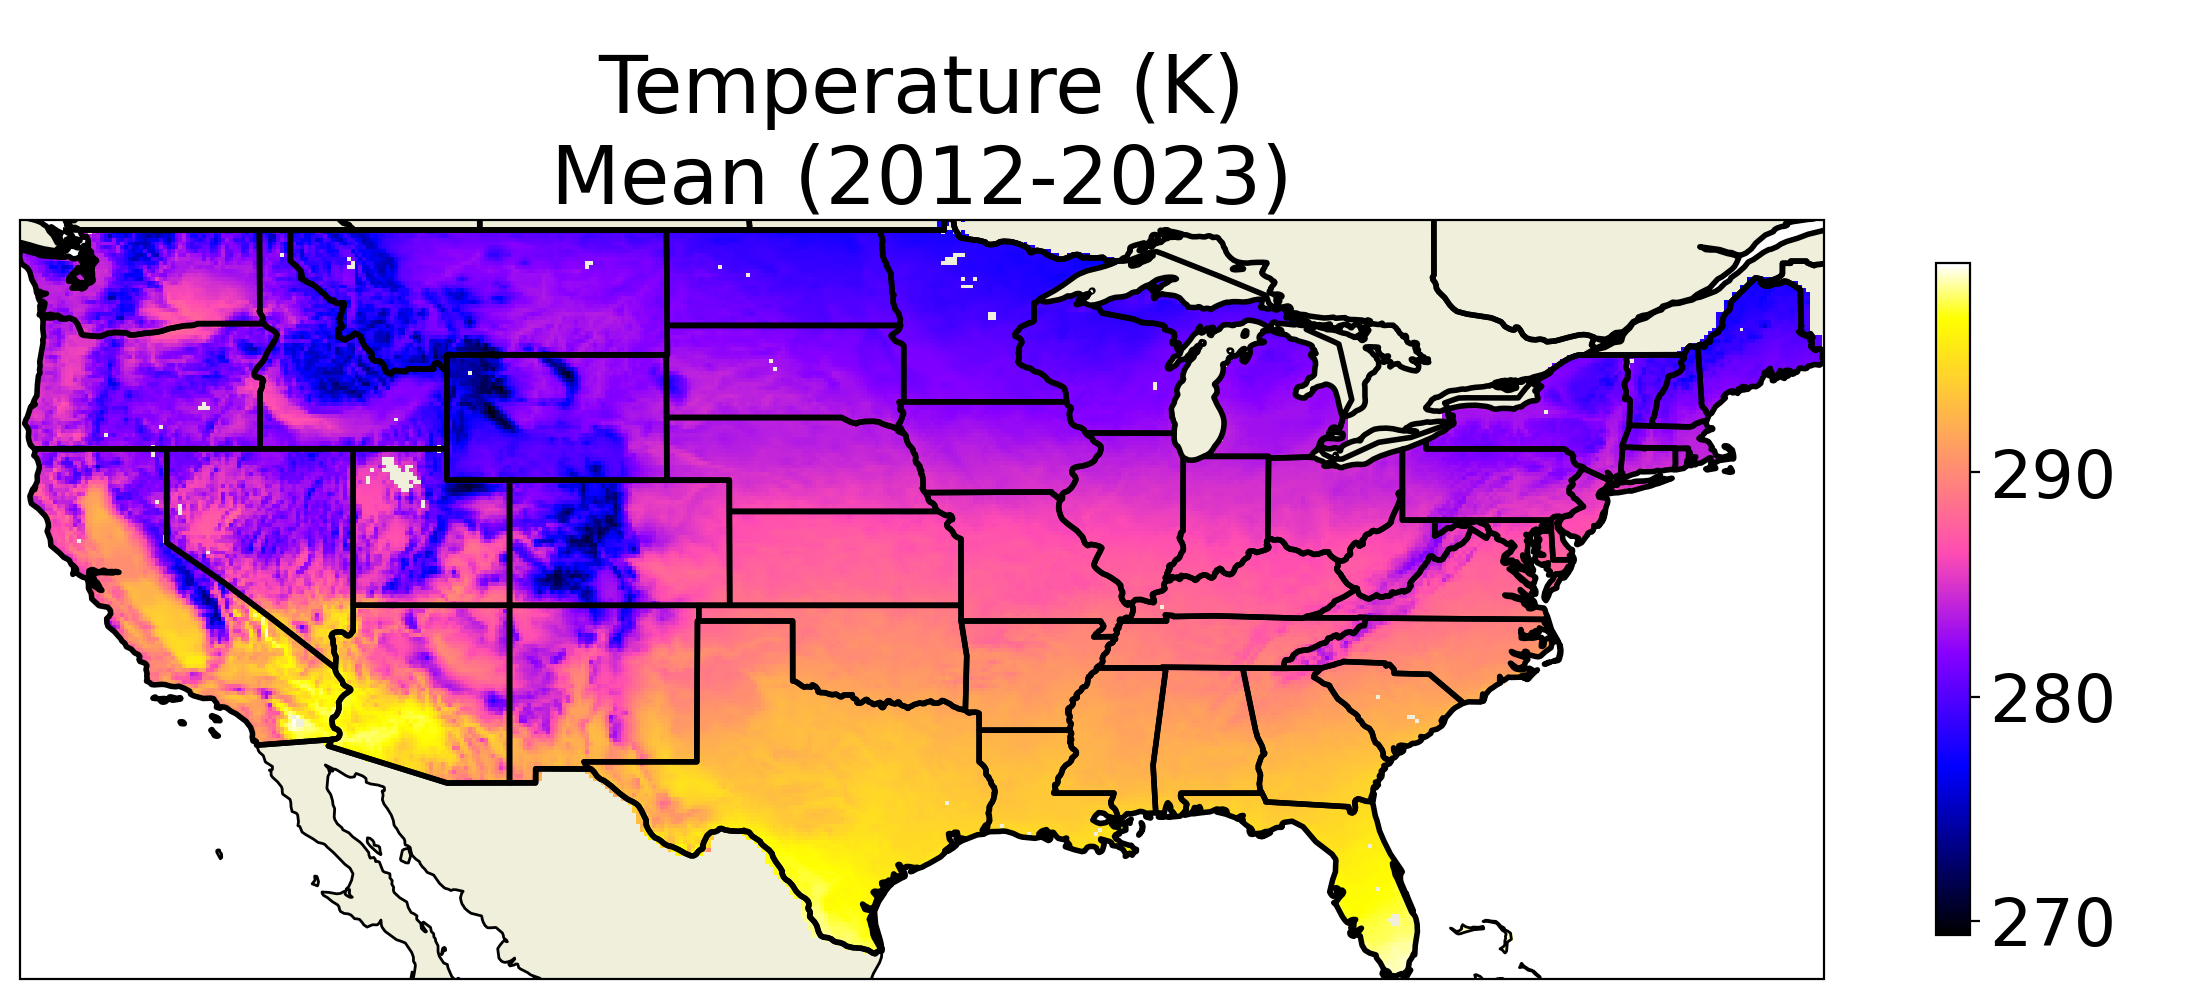
\includegraphics[width=.48\linewidth]{figures/thesis-gridstats/gridstat-bulk_tmp_2012-1_2023-12_y000-195_x000-462_mean.png}
    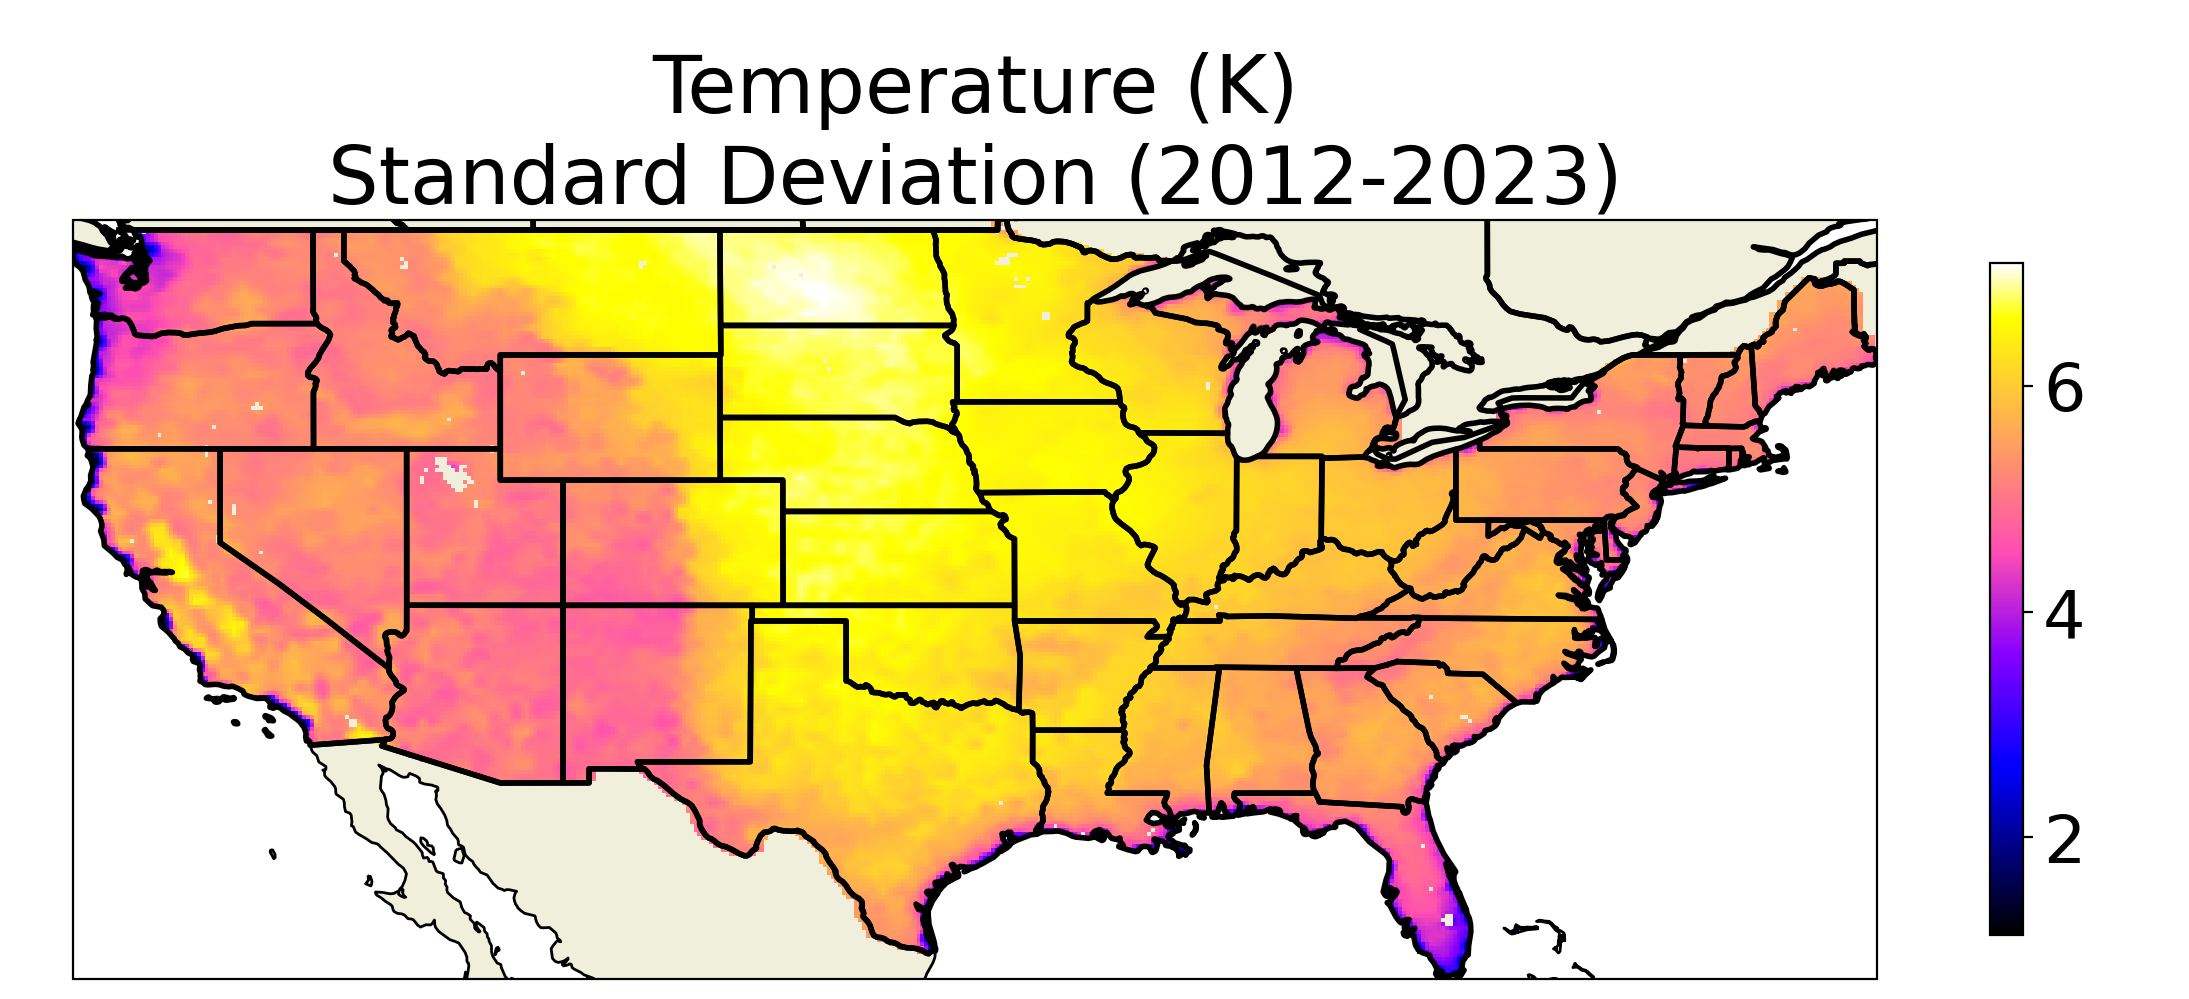
\includegraphics[width=.48\linewidth]{figures/thesis-gridstats/gridstat-bulk_tmp_2012-1_2023-12_y000-195_x000-462_stdev.png}

    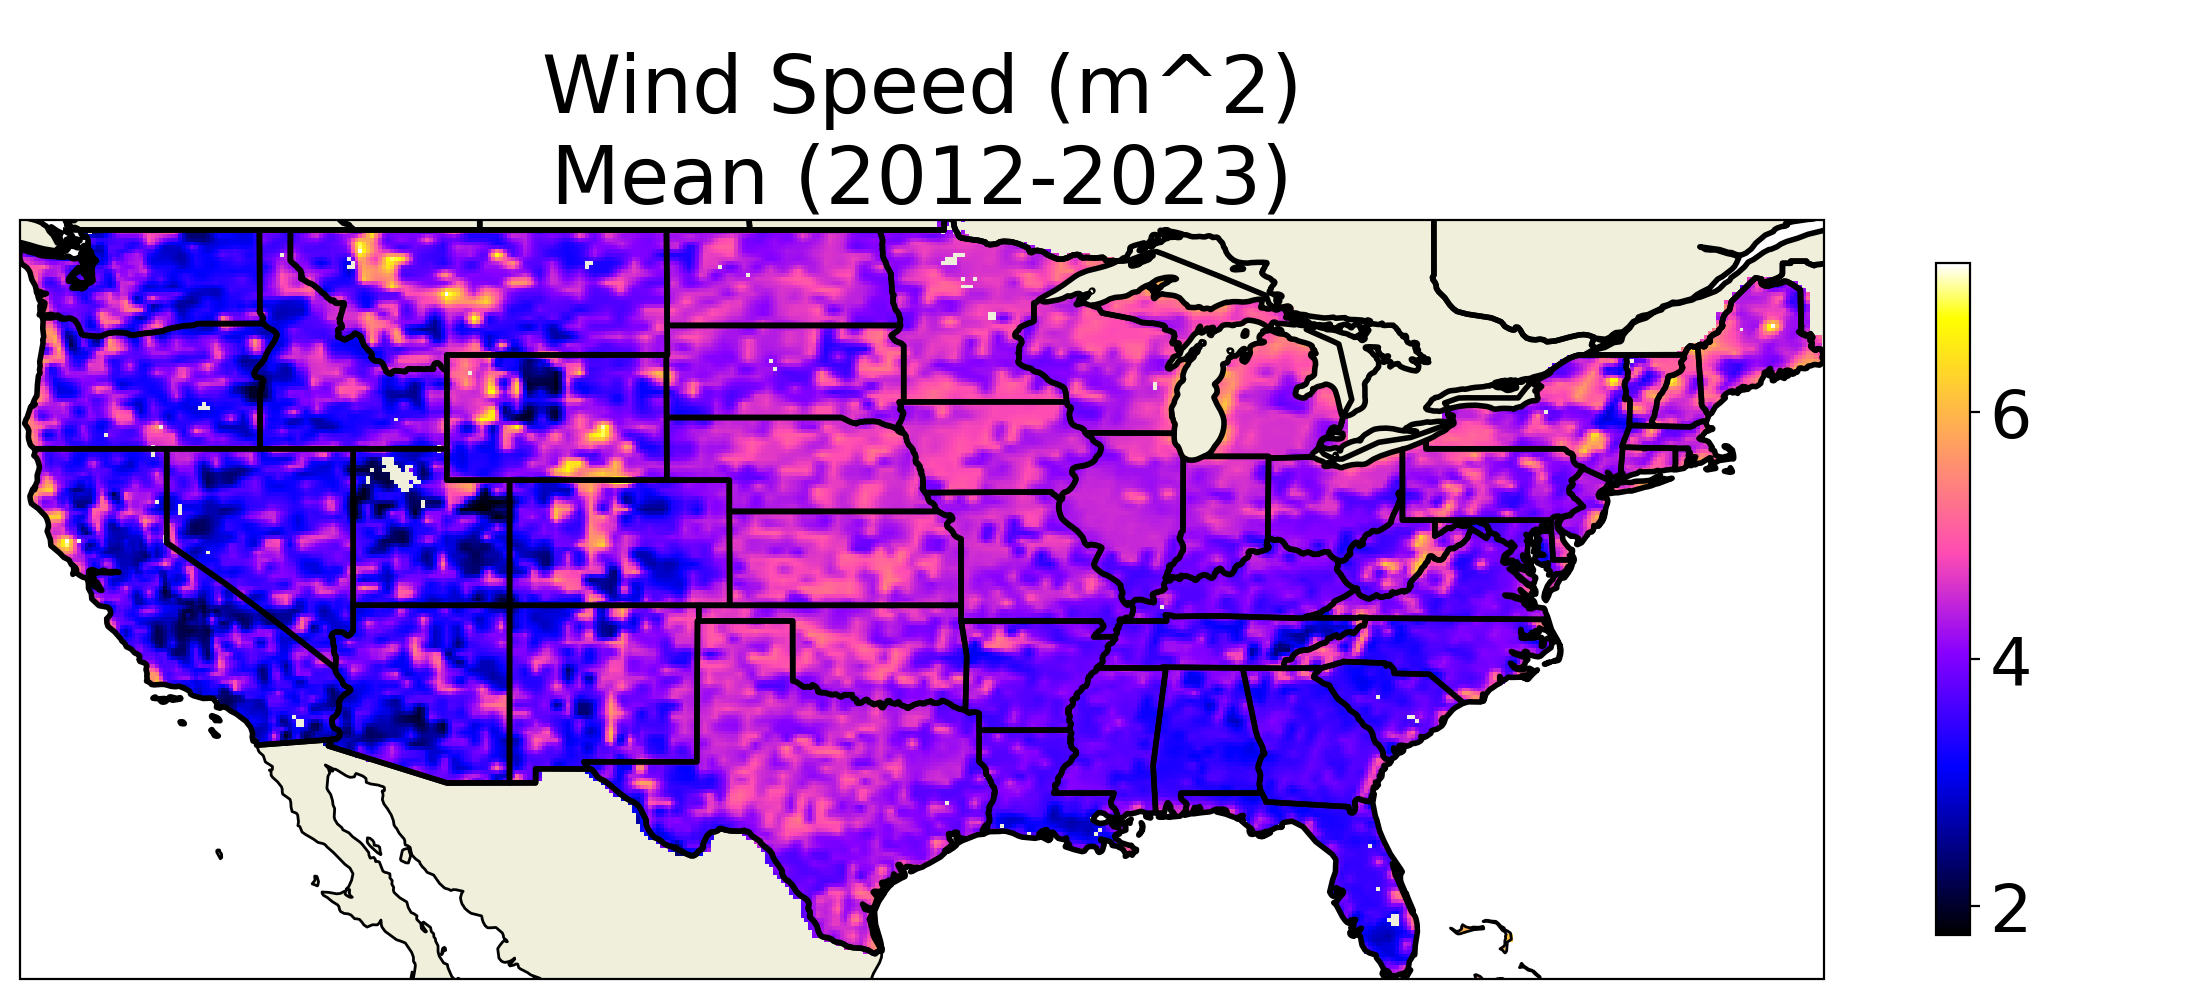
\includegraphics[width=.48\linewidth]{figures/thesis-gridstats/gridstat-bulk_windmag_2012-1_2023-12_y000-195_x000-462_mean.png}
    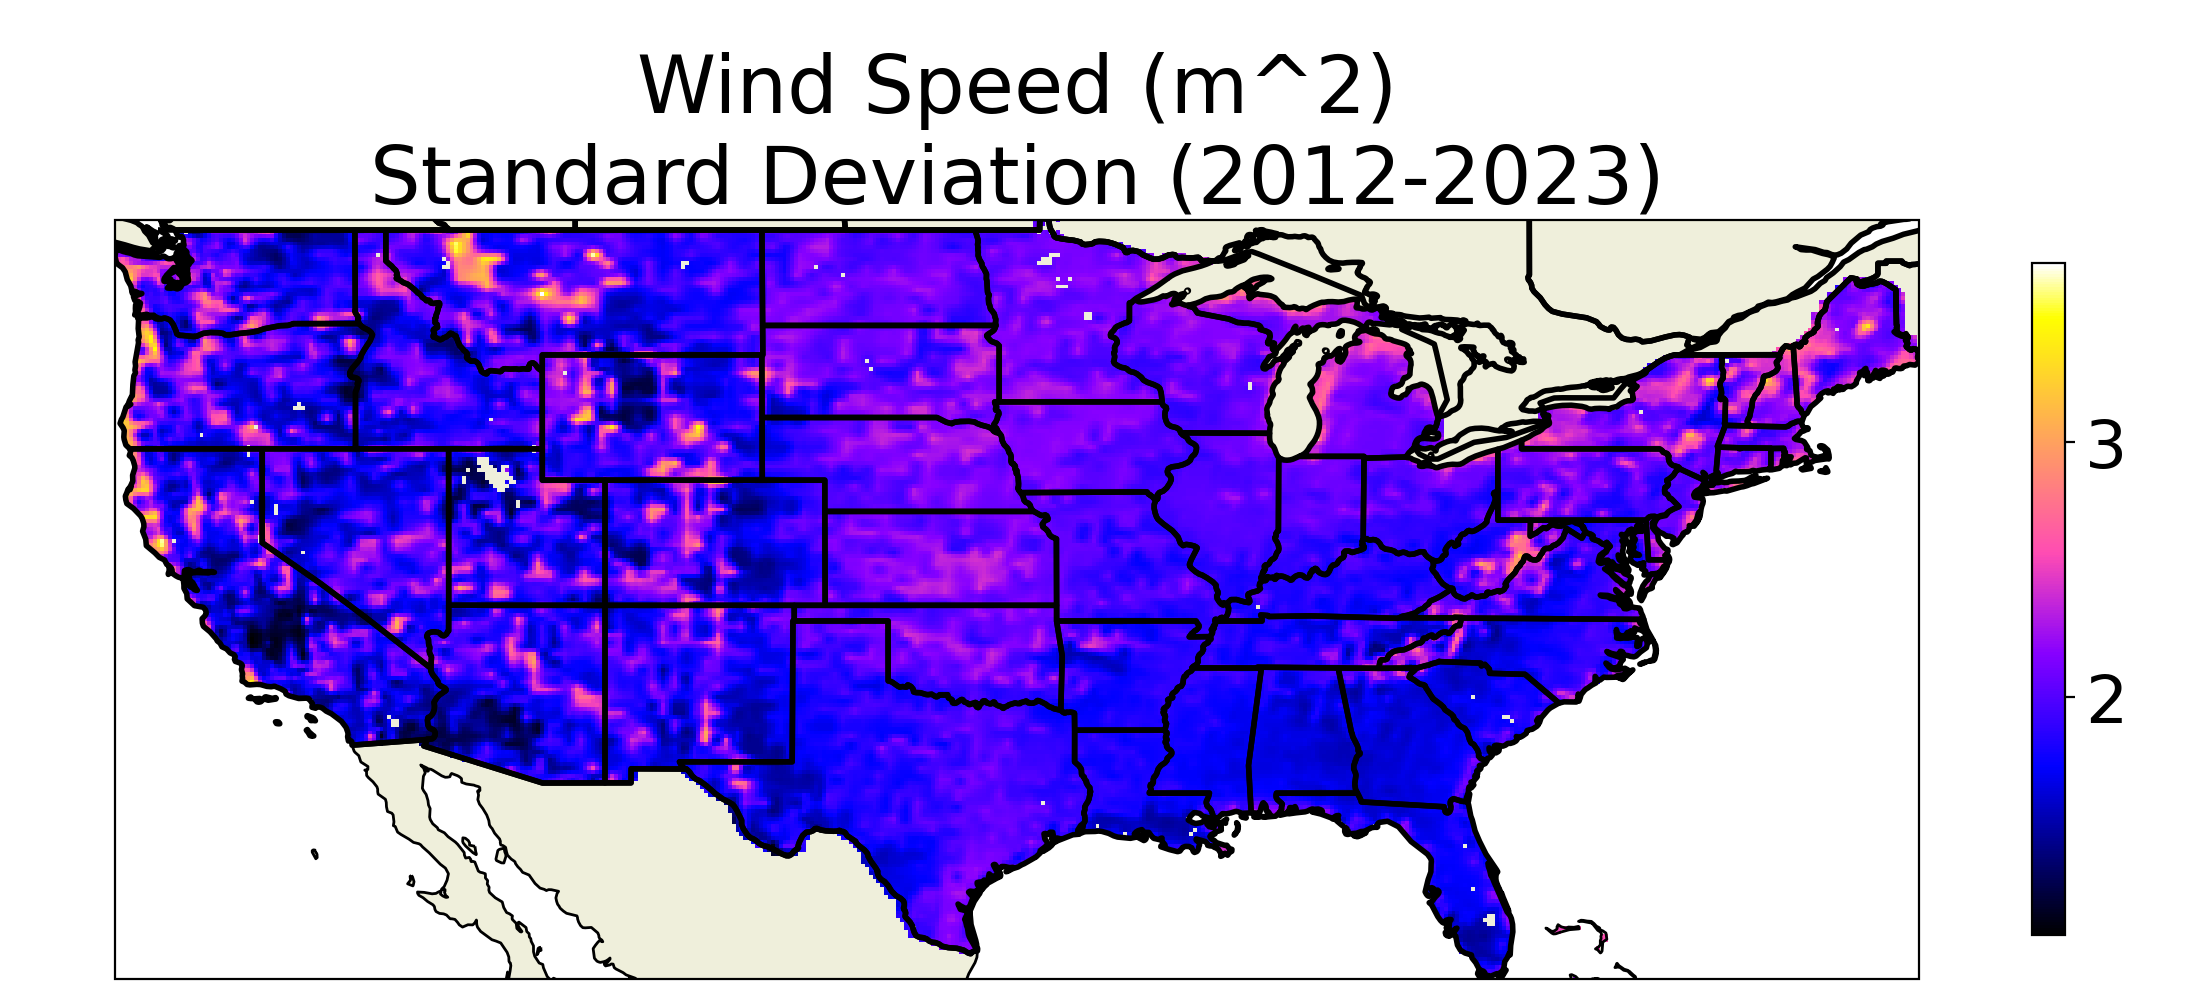
\includegraphics[width=.48\linewidth]{figures/thesis-gridstats/gridstat-bulk_windmag_2012-1_2023-12_y000-195_x000-462_stdev.png}
    \caption{Gridded mean and standard deviation of input forcings (2012-2023)}
    \label{gs-forcings}
\end{figure}

Figure \ref{gs-forcings} displays the same statistics for each of the other input forcings. The precipitation dataset includes liquid rain and snow, and reflects that the highest average values fell in the Pacific Coastal, Cascade, and Sierra Nevada, followed by more moderate values in the broad expanse of the Southeast, with the deep south of Louisiana and Mississippi seeing the strongest variability in precipitation throughout the year. Pressure mainly correlates with altitude, and higher latitudes tend to see the most variance, likely due to the prolonged influence of Rossby waves. Humidity and temperature also strongly correlate with temperature and proximity to the warm gulf, where the highest humidity variance is in the southern states thanks to seasonal intrusions of warm, moist air. The highest temperature variance is found in the high plains where there are considerable intrusions of arctic air in the winter, and solar heating combined with warm air advection from the terrain-driven low level jet in the summer. The wind is locally strongest where there is channeling from mountain slopes, with a broad region of relatively high wind speeds in the plains due to the open terrain.

\subsection{Handling Snow}

\begin{figure}[hb!]
    \centering
    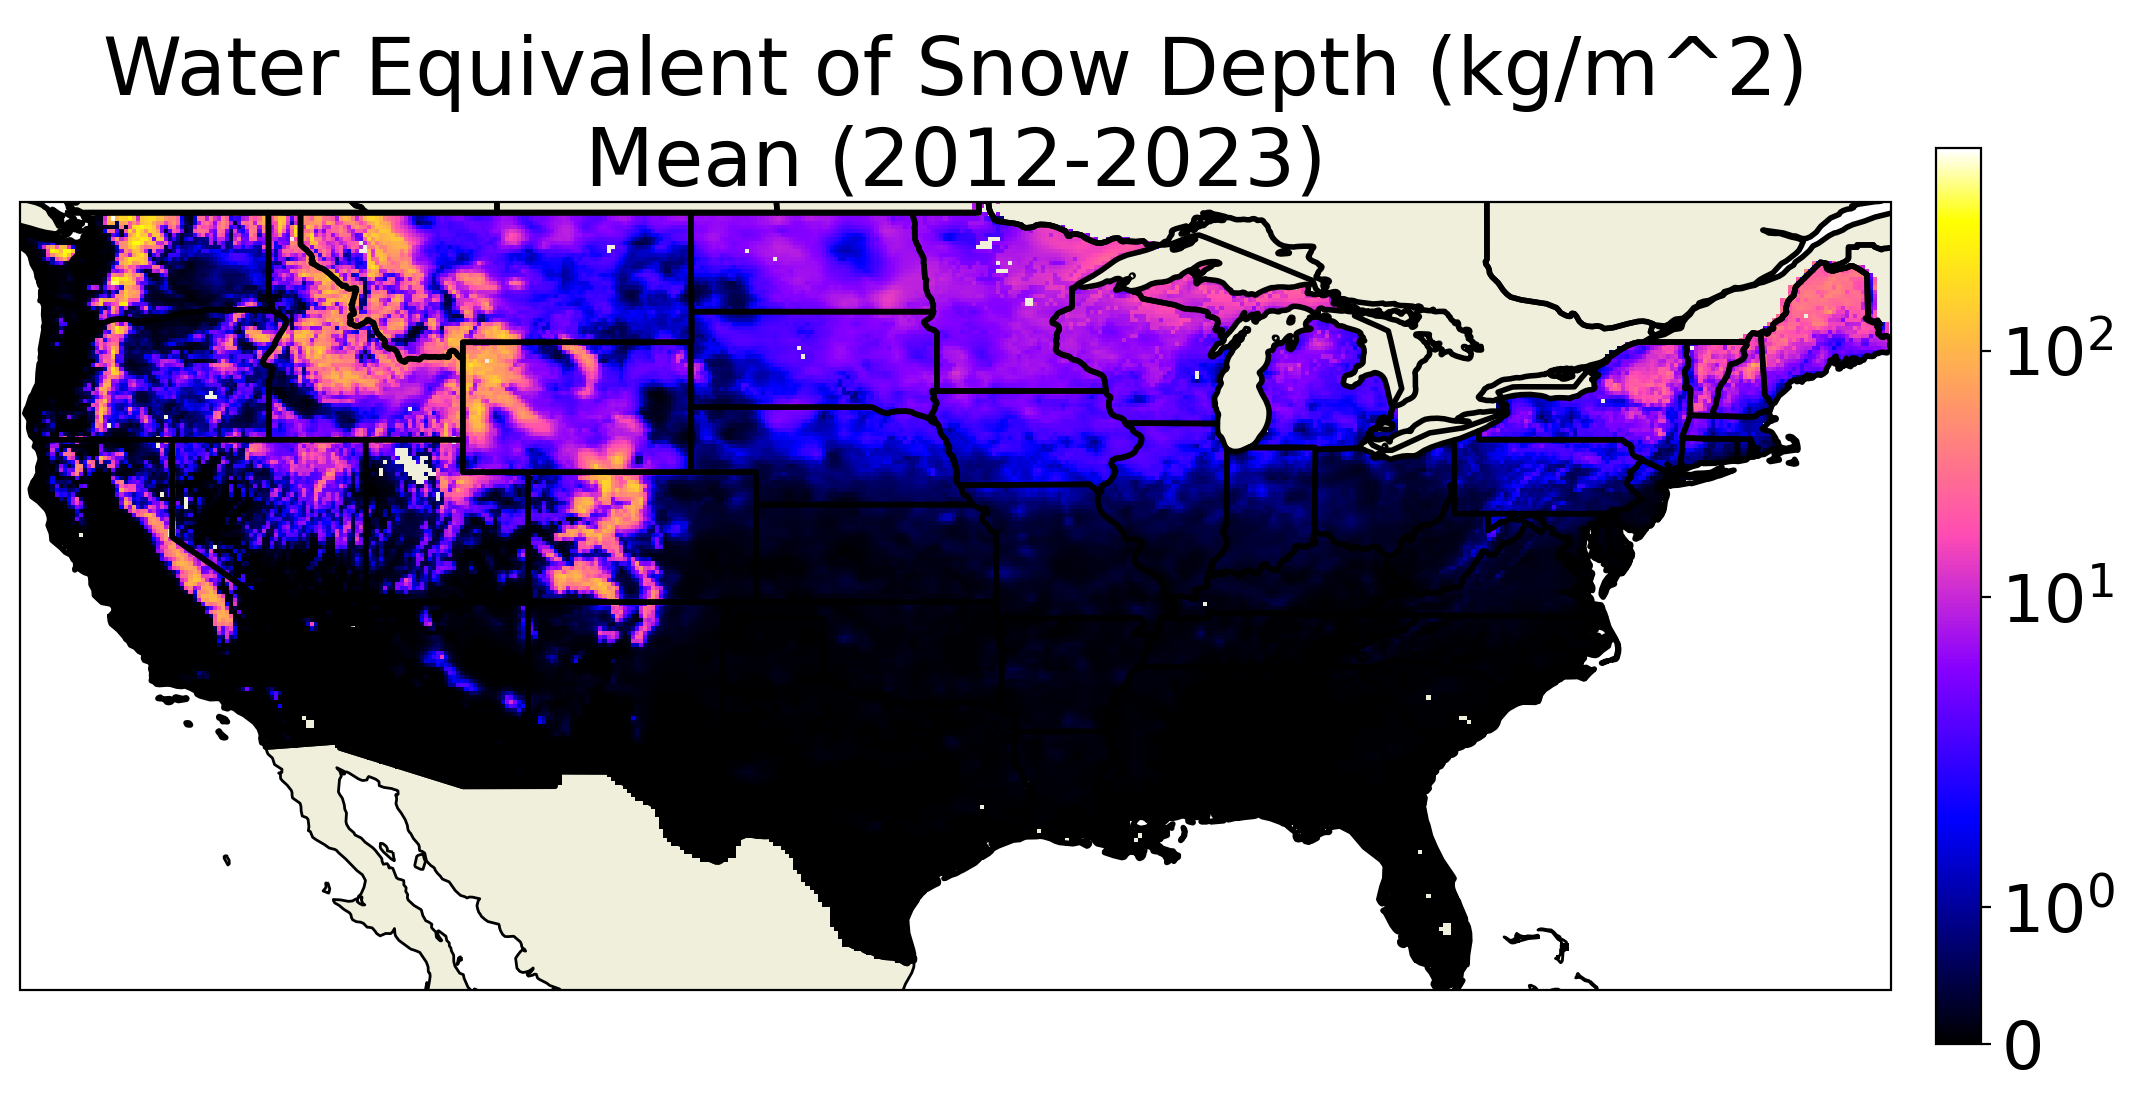
\includegraphics[width=.48\linewidth]{figures/thesis-gridstats/gridstat-bulk_weasd-log_2012-1_2023-12_y000-195_x000-462_mean.png}
    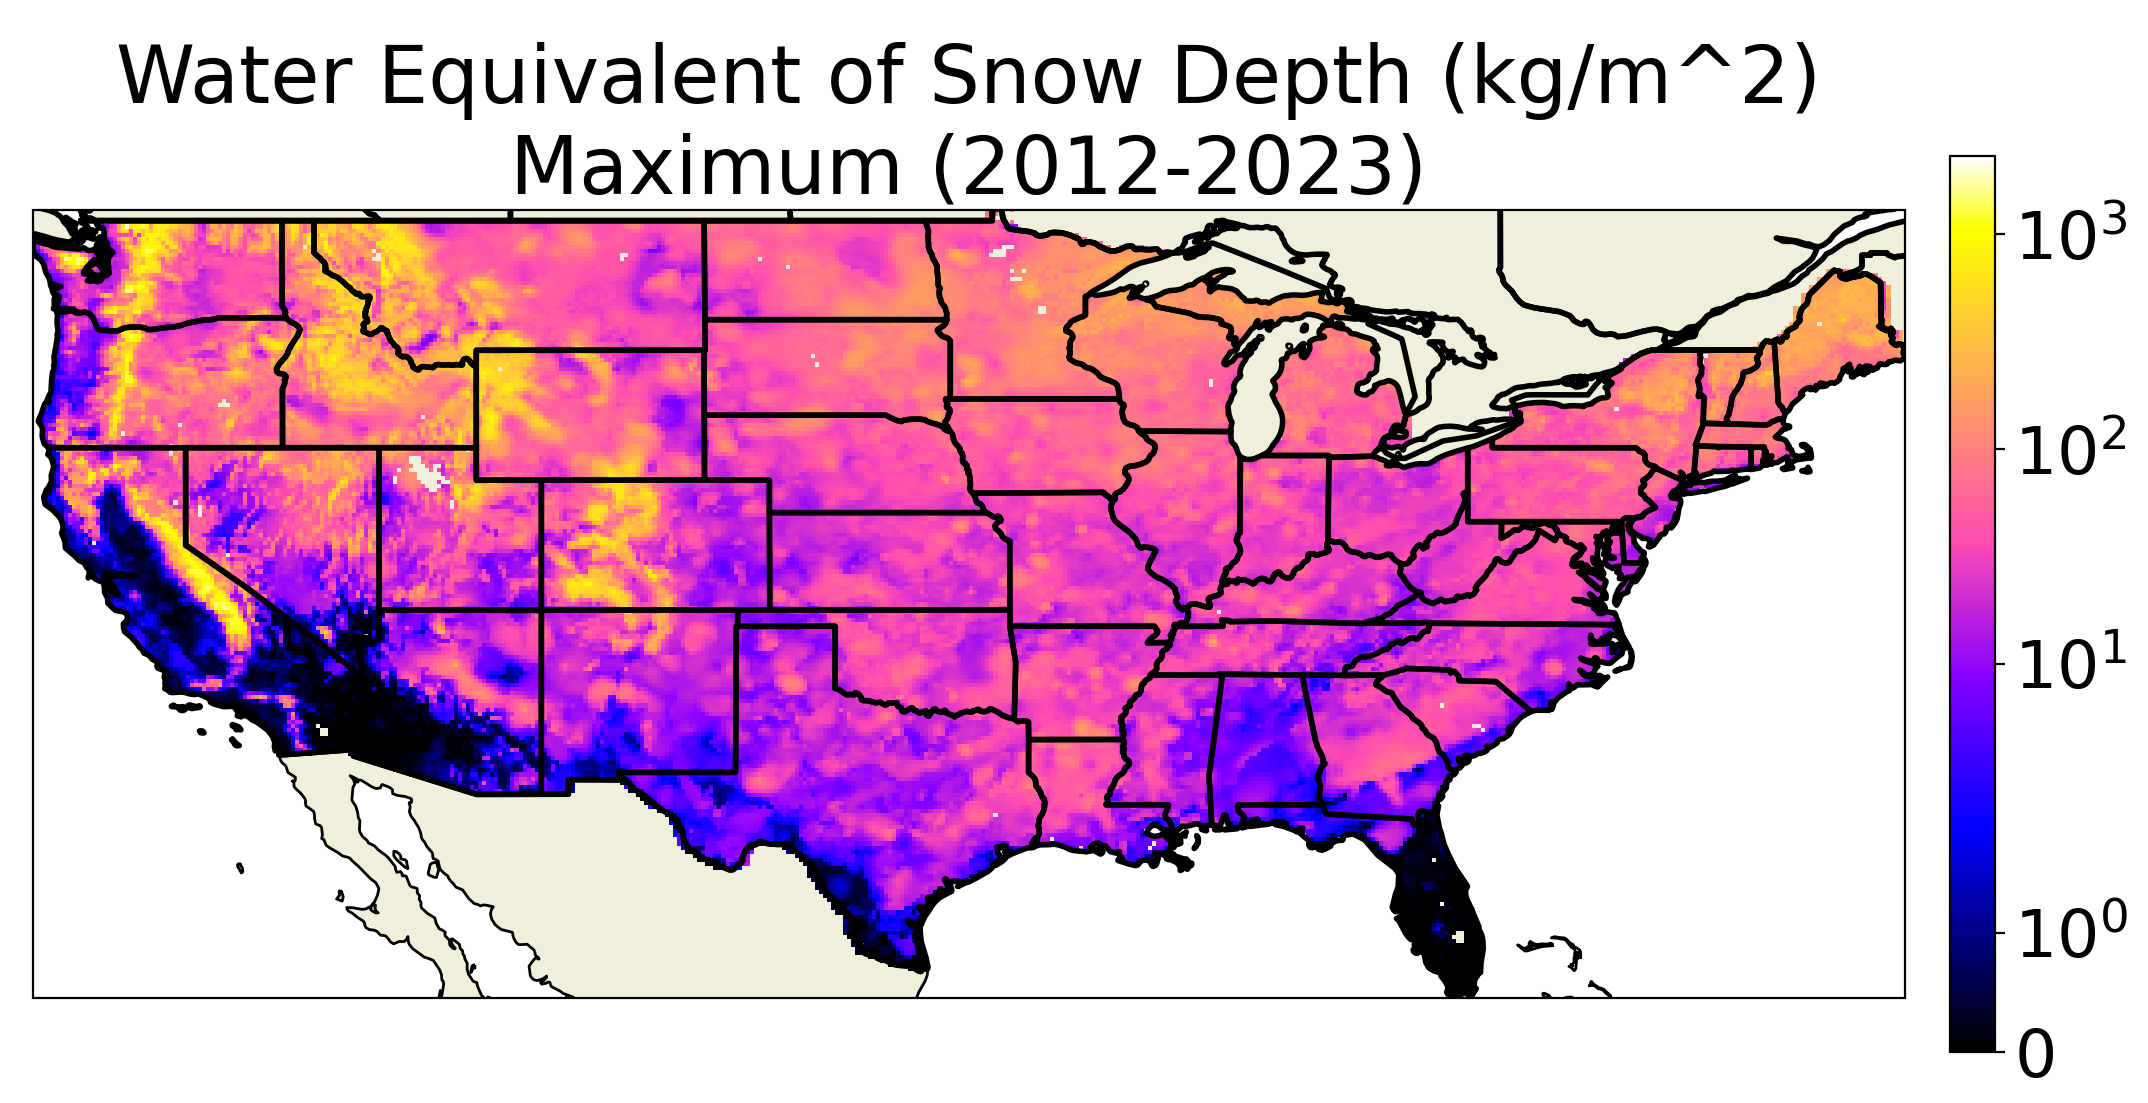
\includegraphics[width=.48\linewidth]{figures/thesis-gridstats/gridstat-bulk_weasd-log_2012-1_2023-12_y000-195_x000-462_max.png}
    \caption{Mean and maximum accumulated snow amounts on a log scale (2012-2023)}
    \label{gs-snow}
\end{figure}

Figure \ref{gs-snow} shows the mean and maximum snow accumulation throughout the dataset. Snow is particularly difficult to account for in the ANNs because it is relatively rare and highly regional, but has a profound influence on the soil dynamics. The presence of snow significantly modifies the surface albedo and roughness length, captures and stores precipitation as an additional state variable, and represents a new source of water for the soil column as it melts. The first exploratory models we trained treated snow as essentially an additional soil layer, and predicted the increment change in its value alongside the other soil states. Since snow is such a transient phenonmenon within the training dataset the ANNs would consistently predict close to zero change, even in snowy conditions, since doing so results in the lowest loss in most cases.

\begin{figure}[hb!]
    \centering
    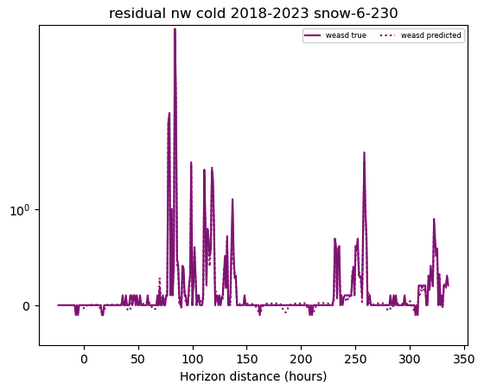
\includegraphics[width=.32\linewidth]{figures/snow-sample_res.png}
    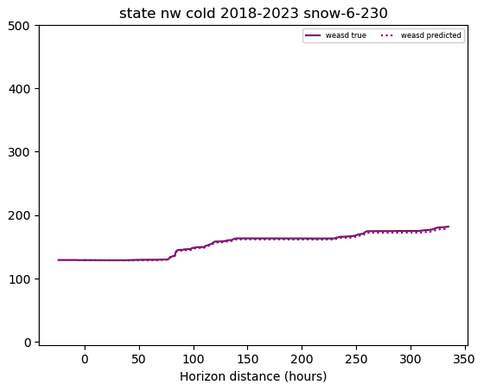
\includegraphics[width=.32\linewidth]{figures/snow-sample_state.png}
    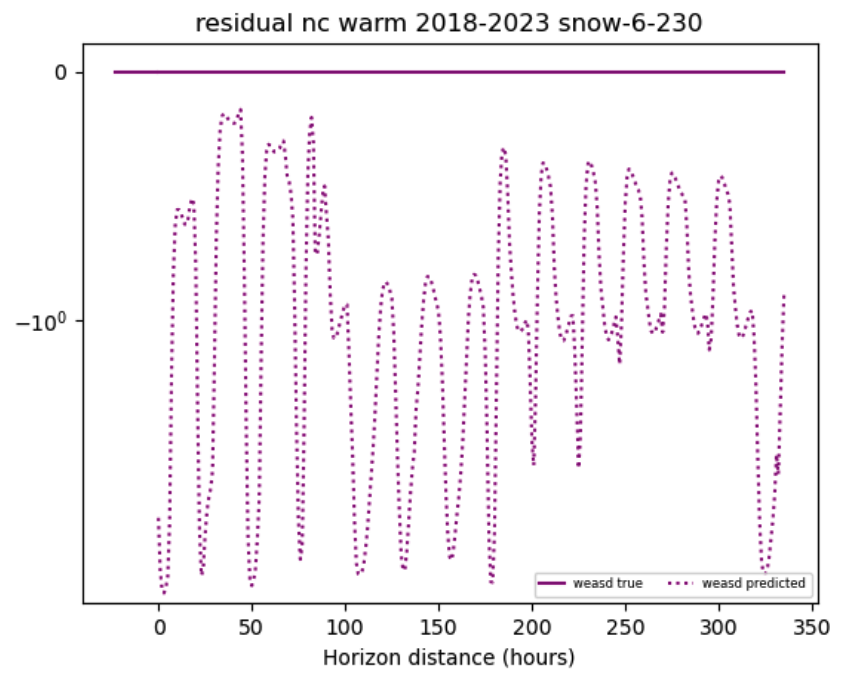
\includegraphics[width=.32\linewidth]{figures/snow-sample_warm.png}
    \caption{Samples of snow-only model predictions vs true values after loss function manipulation, including the increment change for a significant snowfall event (left), the accumulated state for the same sample (center), and an example of the increment outputs of a different warm-season sample (right).}
    \label{snow-models}
\end{figure}

Subsequent models trained to exclusively target the increment change in snow water equivalent showed the same hesitancy to make non-zero predictions. In order to loosen the requirement that these models must always output zero change when there is no snow present, we modified the loss function used to train the snow-only models such that predicting negative increment change values when there is no snow present will not be penalized. When combined with a post-processing step that truncates negative accumulated snow amounts at zero, this strategy focuses the gradient descent process exclusively on samples where the snow pack is relevant.

Figure \ref{snow-models} displays a sample from one of these loss-modified snow models, which captures the subtleties of extreme snow events, and maintains negative increment predictions when there is no snow present or accumulating. Curiously, the negative predictions of the model during the warm-season sample cycle on a diurnal basis, and may represent a hypothetical snow melt rate, which is an emergent property since the loss function wasn't applied in such scenarios. In any case, although these are encouraging preliminary results, further refinement of this strategy is out of the scope of this project. We will use the true snow amount as an input to the soil moisture ANNs presented here in order to prevent compounding error, and take the apparent validity of this approach as an indication that separate ANNs designed specifically for snow water equivalent estimation may be used to initialize soil moisture emulators in the future.

\subsection{Input Data Value Distributions}

\begin{figure}[hb!]
    \centering
    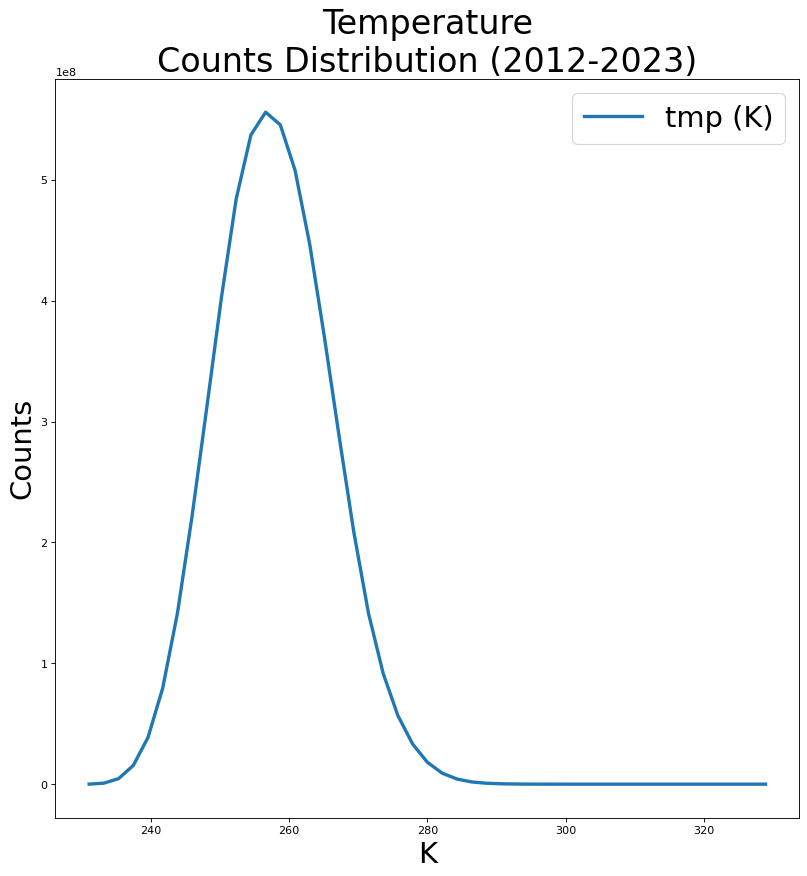
\includegraphics[width=.24\linewidth]{figures/thesis-gridstats/gridstat-hist_tmp_2012-1_2023-12_y000-195_x000-462.png}
    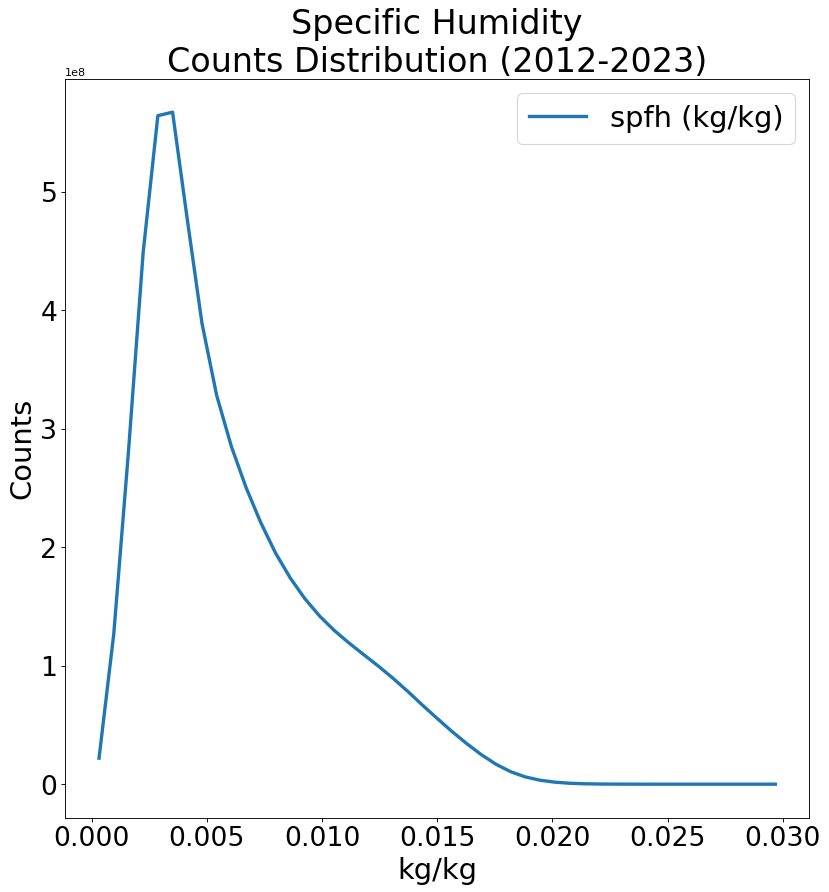
\includegraphics[width=.24\linewidth]{figures/thesis-gridstats/gridstat-hist_spfh_2012-1_2023-12_y000-195_x000-462.png}
    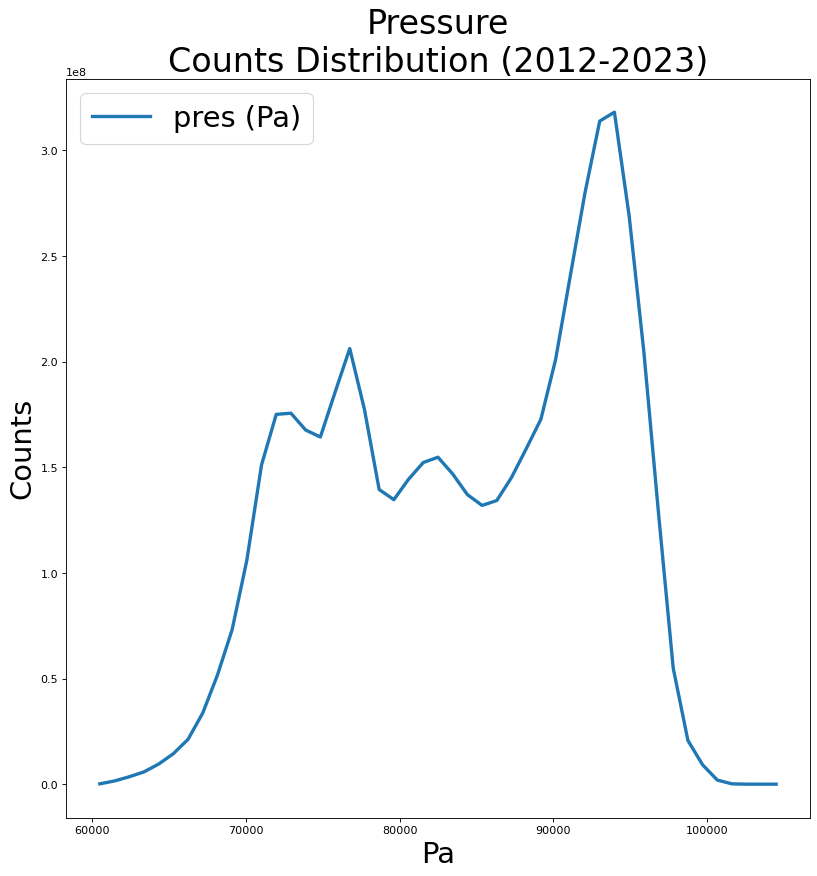
\includegraphics[width=.24\linewidth]{figures/thesis-gridstats/gridstat-hist_pres_2012-1_2023-12_y000-195_x000-462.png}
    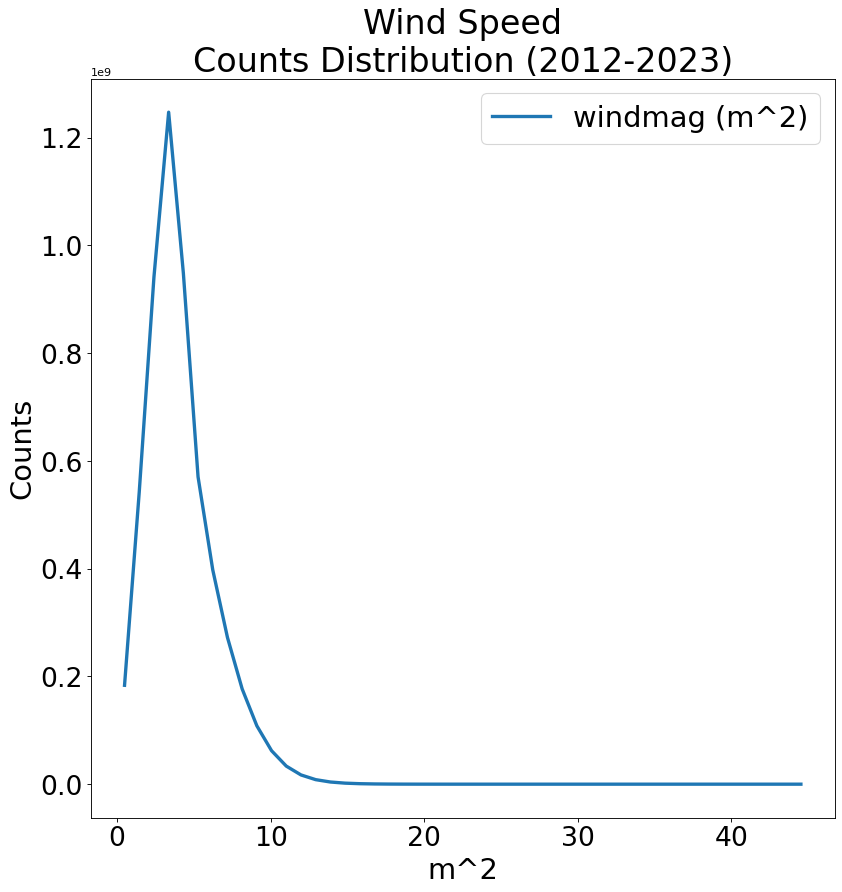
\includegraphics[width=.24\linewidth]{figures/thesis-gridstats/gridstat-hist_windmag_2012-1_2023-12_y000-195_x000-462.png}

    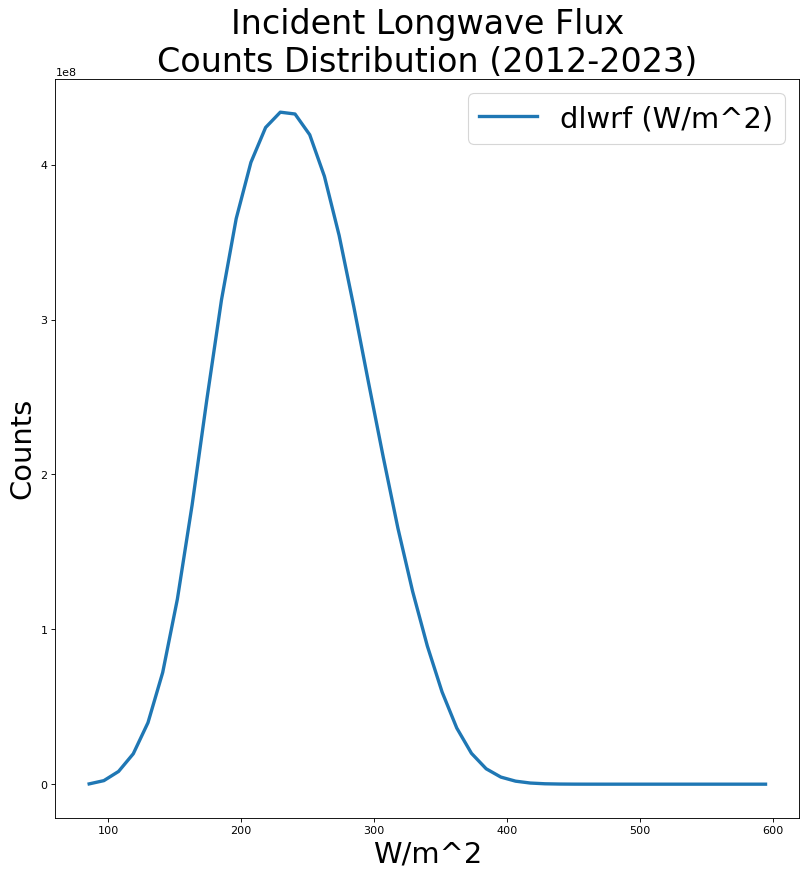
\includegraphics[width=.24\linewidth]{figures/thesis-gridstats/gridstat-hist_dlwrf_2012-1_2023-12_y000-195_x000-462.png}
    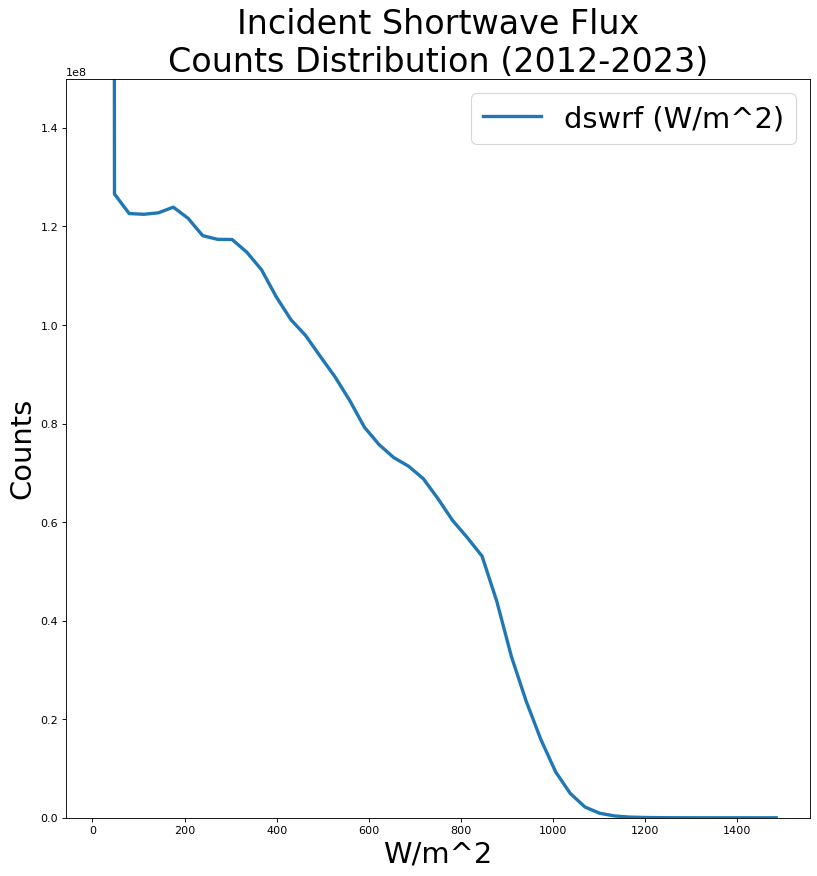
\includegraphics[width=.24\linewidth]{figures/thesis-gridstats/gridstat-hist_dswrf_2012-1_2023-12_y000-195_x000-462.png}
    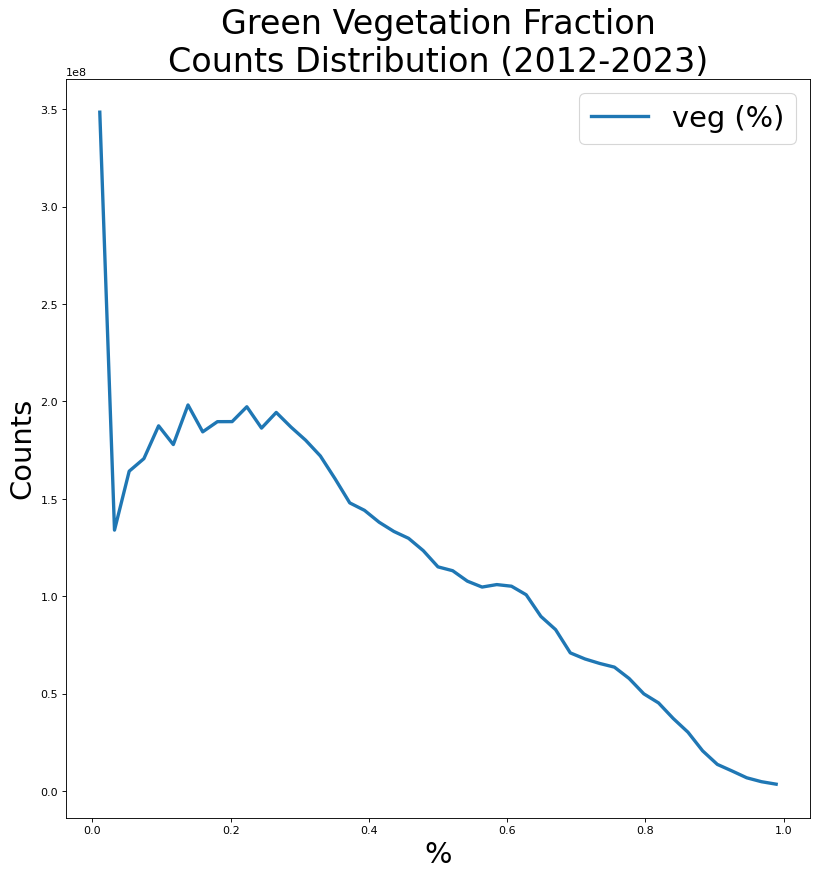
\includegraphics[width=.24\linewidth]{figures/thesis-gridstats/gridstat-hist_veg_2012-1_2023-12_y000-195_x000-462.png}
    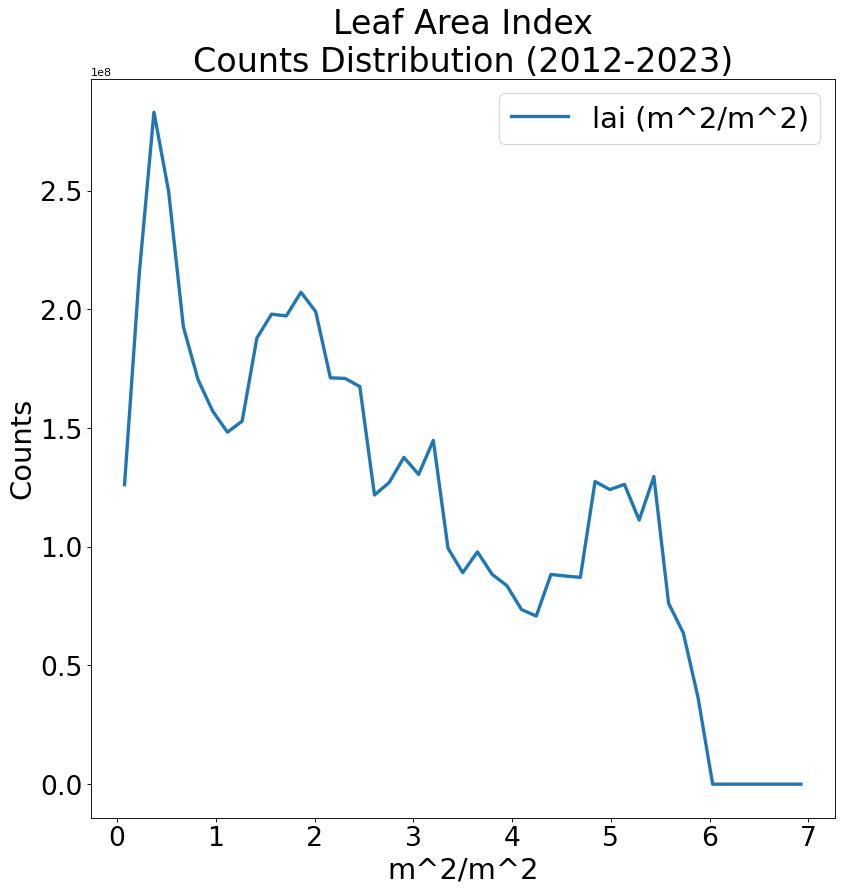
\includegraphics[width=.24\linewidth]{figures/thesis-gridstats/gridstat-hist_lai_2012-1_2023-12_y000-195_x000-462.png}

    \caption{Overall distributions of dynamic model inputs (2012-2023)}
    \label{dist-forcings}
\end{figure}

The count distributions of dynamic inputs with the exception of precipitation are displayed by Figure \ref{dist-forcings}. Of these only temperature and incident longwave flux follow generally gaussian distributions. Specific humidity is strongly skewed toward zero since its upper bound is strongly limited by temperature. Pressure has a global peak just below sea level pressure, with relative maxima associated with the mountainous terrain of Appalachia and the West. Windspeed has a strong peak around 5 $m s^{-1}$, with a long tail of outliers. Shortwave flux is not entirely smooth, which is likely due in part to enhanced cloud cover from orographic effects, judging by the spatial distribution in Figure \ref{gs-radiative}. The vegetation parameters are also strongly non-gaussian owing to their regional and seasonal heterogeneity, and the discrete differences in vegetation categories.


\begin{figure}[h!]
    \centering
    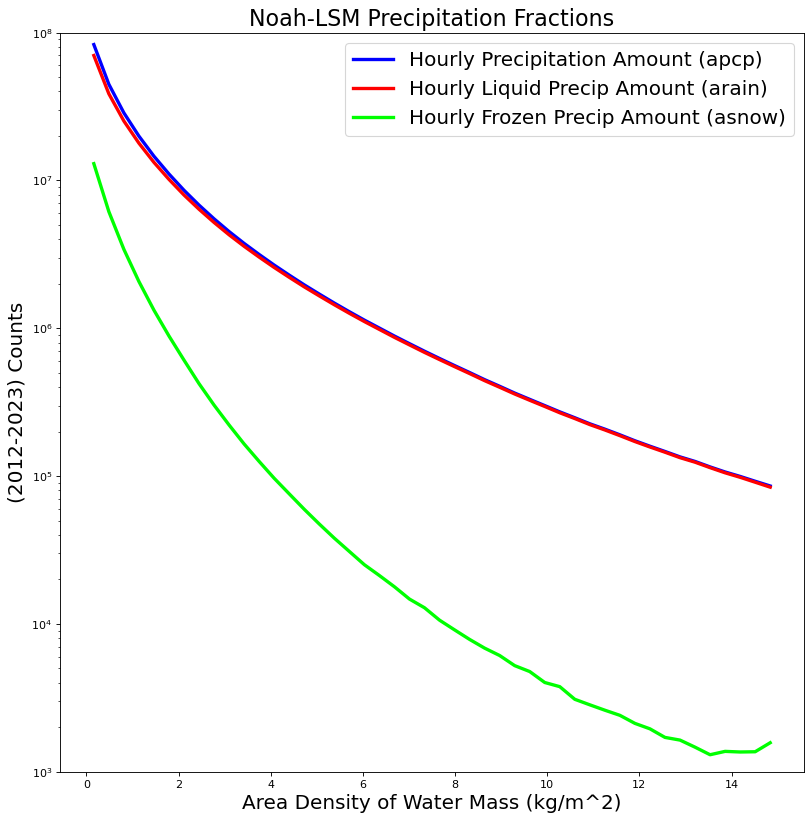
\includegraphics[width=.48\linewidth]{figures/thesis-gridstats/gridstat-hist_groupings_preciptype.png}
    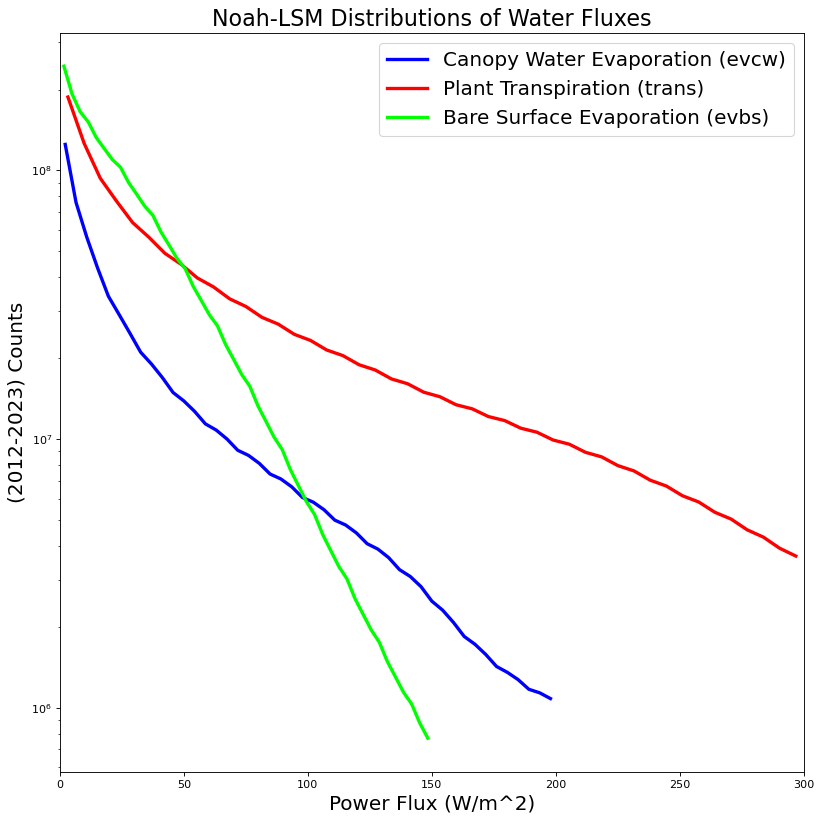
\includegraphics[width=.48\linewidth]{figures/thesis-gridstats/gridstat-hist_groupings_powerflux.png}
    \caption{Overall distributions of precipitation types (left) and fluxes removing water from the surface system (right), both on a logarithmic axis (2012-2023).}
    \label{dist-waterflux}
\end{figure}

Figure \ref{dist-waterflux} compares the distributions of precipitation types, and those of the fluxes that remove water from the system. Liquid precipitation represents the vast majority of the total hourly precipitation amount, especially for strong precipitation events. Plant transpiration is the dominant sink for soil moisture content, with bare surface evaporation mainly limited to lower rates. Evaporation from the plant canopy can also be relevant in mitigating the amount of water that percolated downward into the soil column after rain events. Each of the distributions extend further with higher-value outliers, however these were truncated during the statistic collection process in order to emphasize the shape of the more common lower-end values. Notice that all of these processes are plotted on a log axis in the figure for visual clarity, which belies the fact that these are extremely skewed distributions. Similar to snow as outlined in the previous subsection, although they are important processes within the model, the fluxes and precipitation -- and especially their upper extremes -- are ultimately rare in the context of the full dataset, which poses a challenge for statistical optimization techniques like deep learning.

\subsection{Soil Moisture Distribution and Metrics}

\begin{figure}[h!]
    \centering
    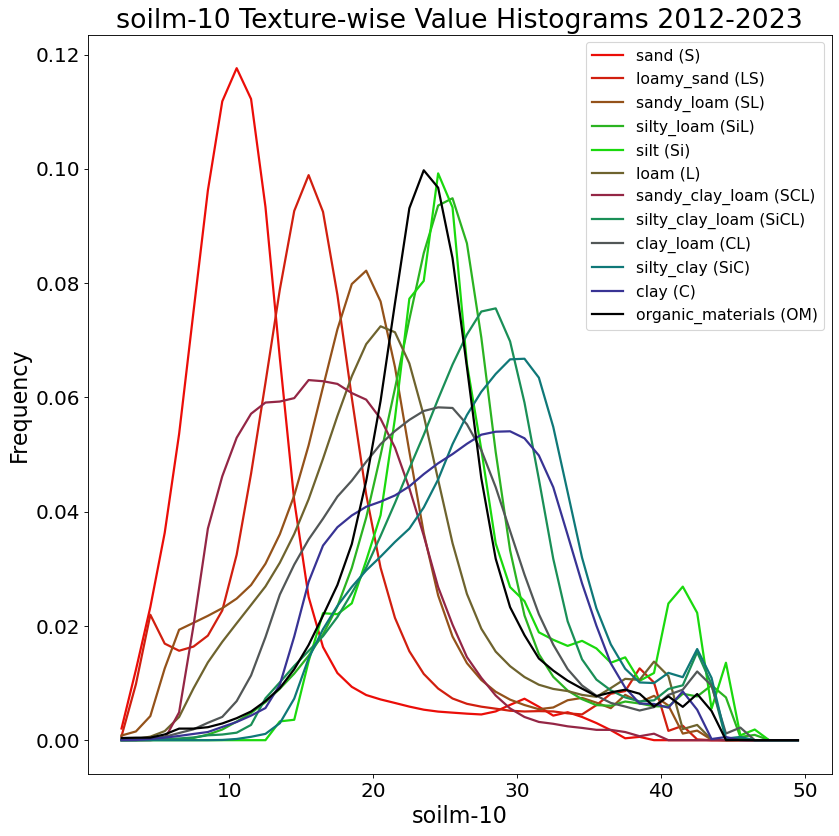
\includegraphics[width=.32\linewidth]{figures/thesis-gridstats/gridstat-hist-textures_soilm-10_2012-1_2023-12_y000-195_x000-462}
    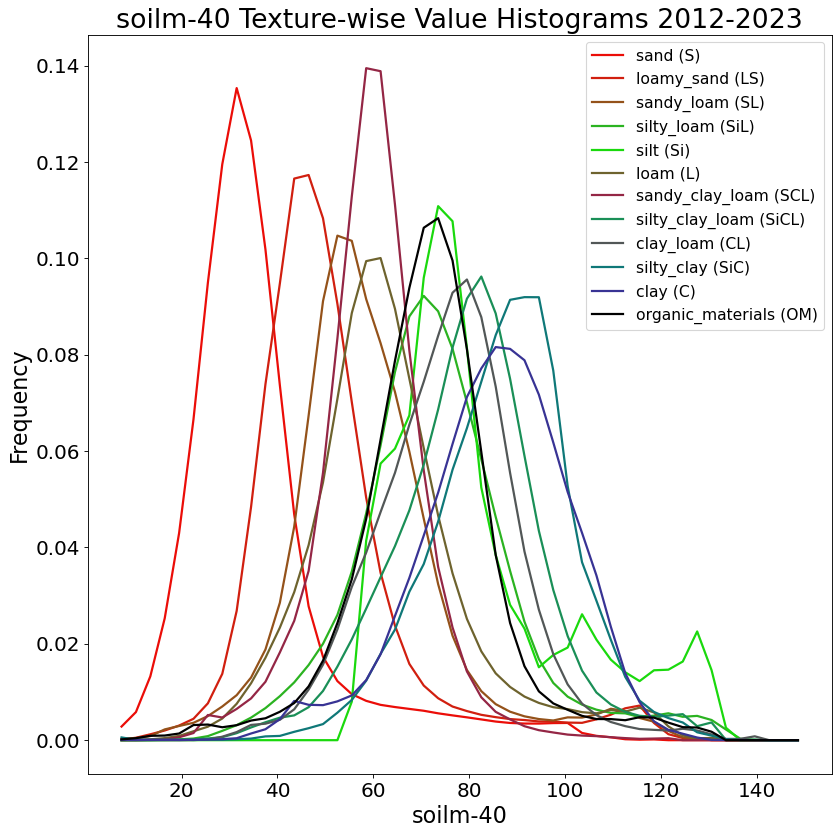
\includegraphics[width=.32\linewidth]{figures/thesis-gridstats/gridstat-hist-textures_soilm-40_2012-1_2023-12_y000-195_x000-462}
    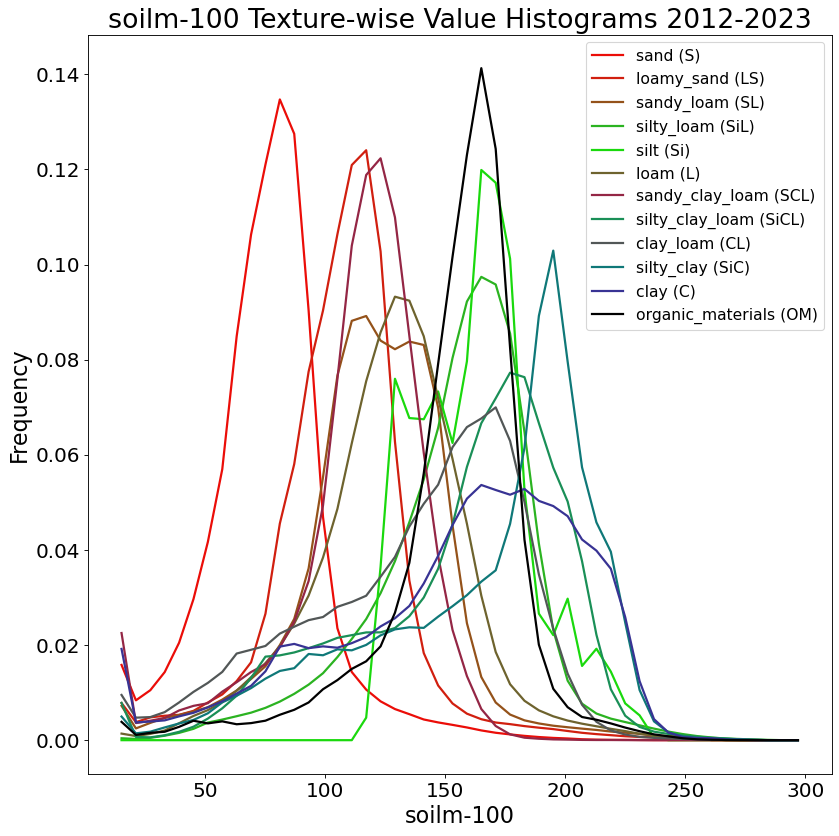
\includegraphics[width=.32\linewidth]{figures/thesis-gridstats/gridstat-hist-textures_soilm-100_2012-1_2023-12_y000-195_x000-462}

    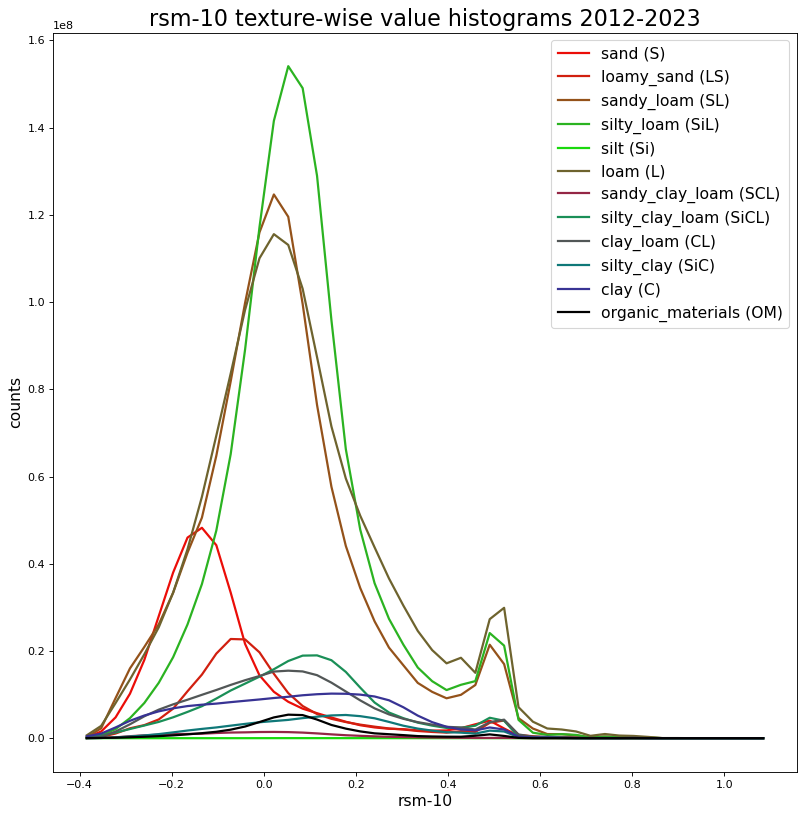
\includegraphics[width=.32\linewidth]{figures/thesis-gridstats/gridstat-hist-textures_rsm-10_2012-1_2023-12_y000-195_x000-462}
    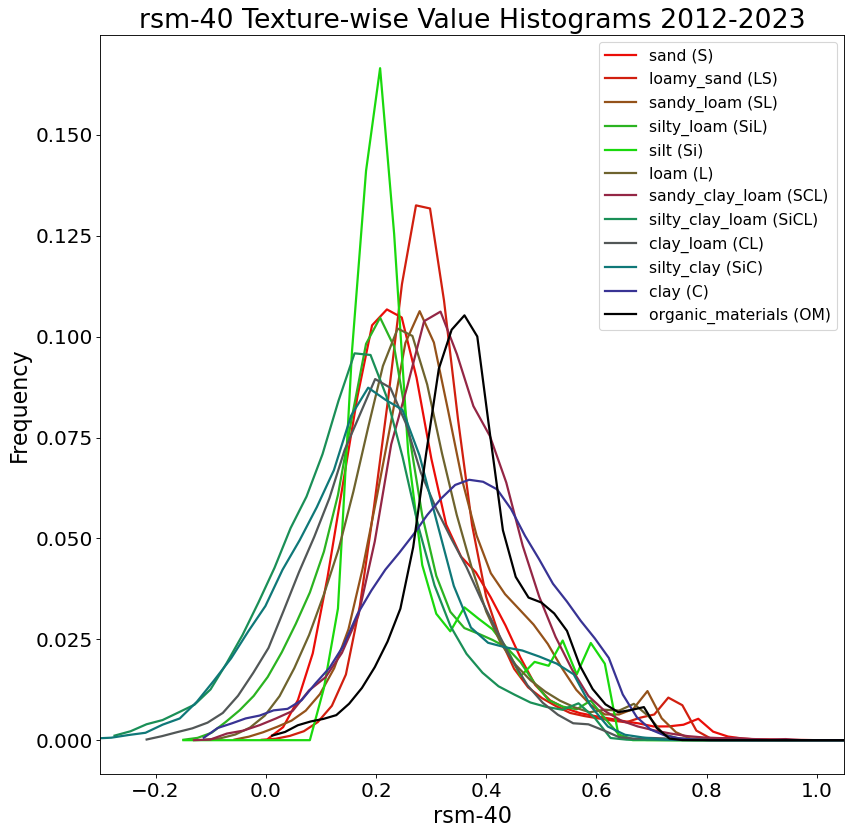
\includegraphics[width=.32\linewidth]{figures/thesis-gridstats/gridstat-hist-textures_rsm-40_2012-1_2023-12_y000-195_x000-462}
    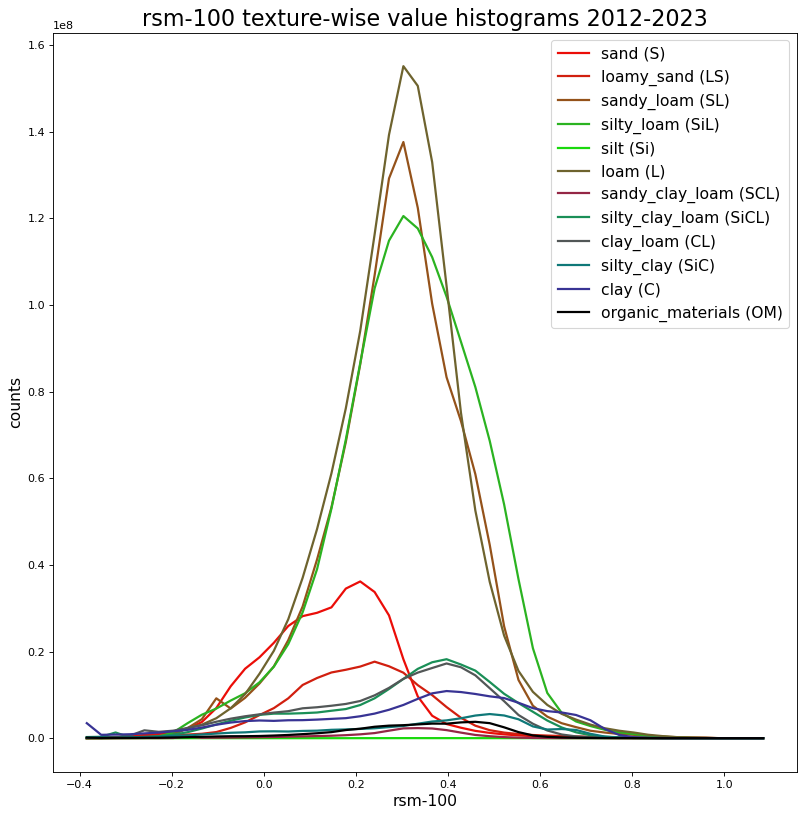
\includegraphics[width=.32\linewidth]{figures/thesis-gridstats/gridstat-hist-textures_rsm-100_2012-1_2023-12_y000-195_x000-462}


    \caption{Distributions of relative soil moisture (top) compared to those of soil moisture area density (bottom) at the first three depth levels, separated by soil texture category. Red, green, and blue components of line colors correspond to the sand, silt, and clay composition of the soil textures, respectively.}
    \label{dist-soilm}
\end{figure}

The differences in conductivity, matric potential, and other hydraulic properties among soil textures causes their distributions to occupy distinct value ranges, and their dynamics to vary at rates that are characteristic to each specific class. As the top row of Figure \ref{gs-rsm} indicates, the distributions of soil moisture area density (in $kg\,m^{-2}$) tends to stratify such that coarser textures (sandy blends) have generally lower moisture content per unit volume, and vice-versa with silt and clay dominant soil textures. Although there is some regional influence, this is mainly owed to the faster percolation rates and lower porosity of the coarser soil.

Since the loss function calculations are directly dependent on the magnitude of soil moisture, we hypothesized that significant differences in these value ranges could diminish the ANNs' ability to learn general solutions that apply to all soil textures. For example, since clay has a slow conductivity and infiltration rate and thus typically smaller magnitudes of increment change, loss calculations based on the increment change would be de-emphasized compared to sand. For this reason, we adopt the relative soil moisture as a physically-interpretable metric for normalizing soil textures to values that occupy roughly the same scale.

\begin{equation}\label{rsm-eq}
    \text{RSM} = \frac{\frac{\text{SOILM}}{d \, \rho_w} - \theta_{wp}}{\theta_s - \theta_{wp}}
\end{equation}

Relative soil moisture (RSM) linearly scales the water content such that each texture's wilting point is at zero, and saturation point corresponds to one. In Equation \ref{rsm-eq}, SOILM is the area density, $\rho_w$ is the density of water, $d$ is the depth of the soil layer, $\theta_s$ is the saturation point of a particular soil texture as a ratio of the total volume, and $\theta_{wp}$ is the wilting point. In this manner, the RSM can never exceed 1, but its lower bound is defined in terms of the hydraulic suction head needed to uptake further water. As such, very dry soils can have RSM values below zero. The layerwise comparisons of SOILM to RSM in Figure \ref{gsm-rsm} make clear how RSM normalization aligns the individual texture distributions, and the added benefit of uniting the separate soil layers to a similar range of state values rather than using mass quantities that scale with their unique depths.

\begin{figure}[h!]
    \centering
    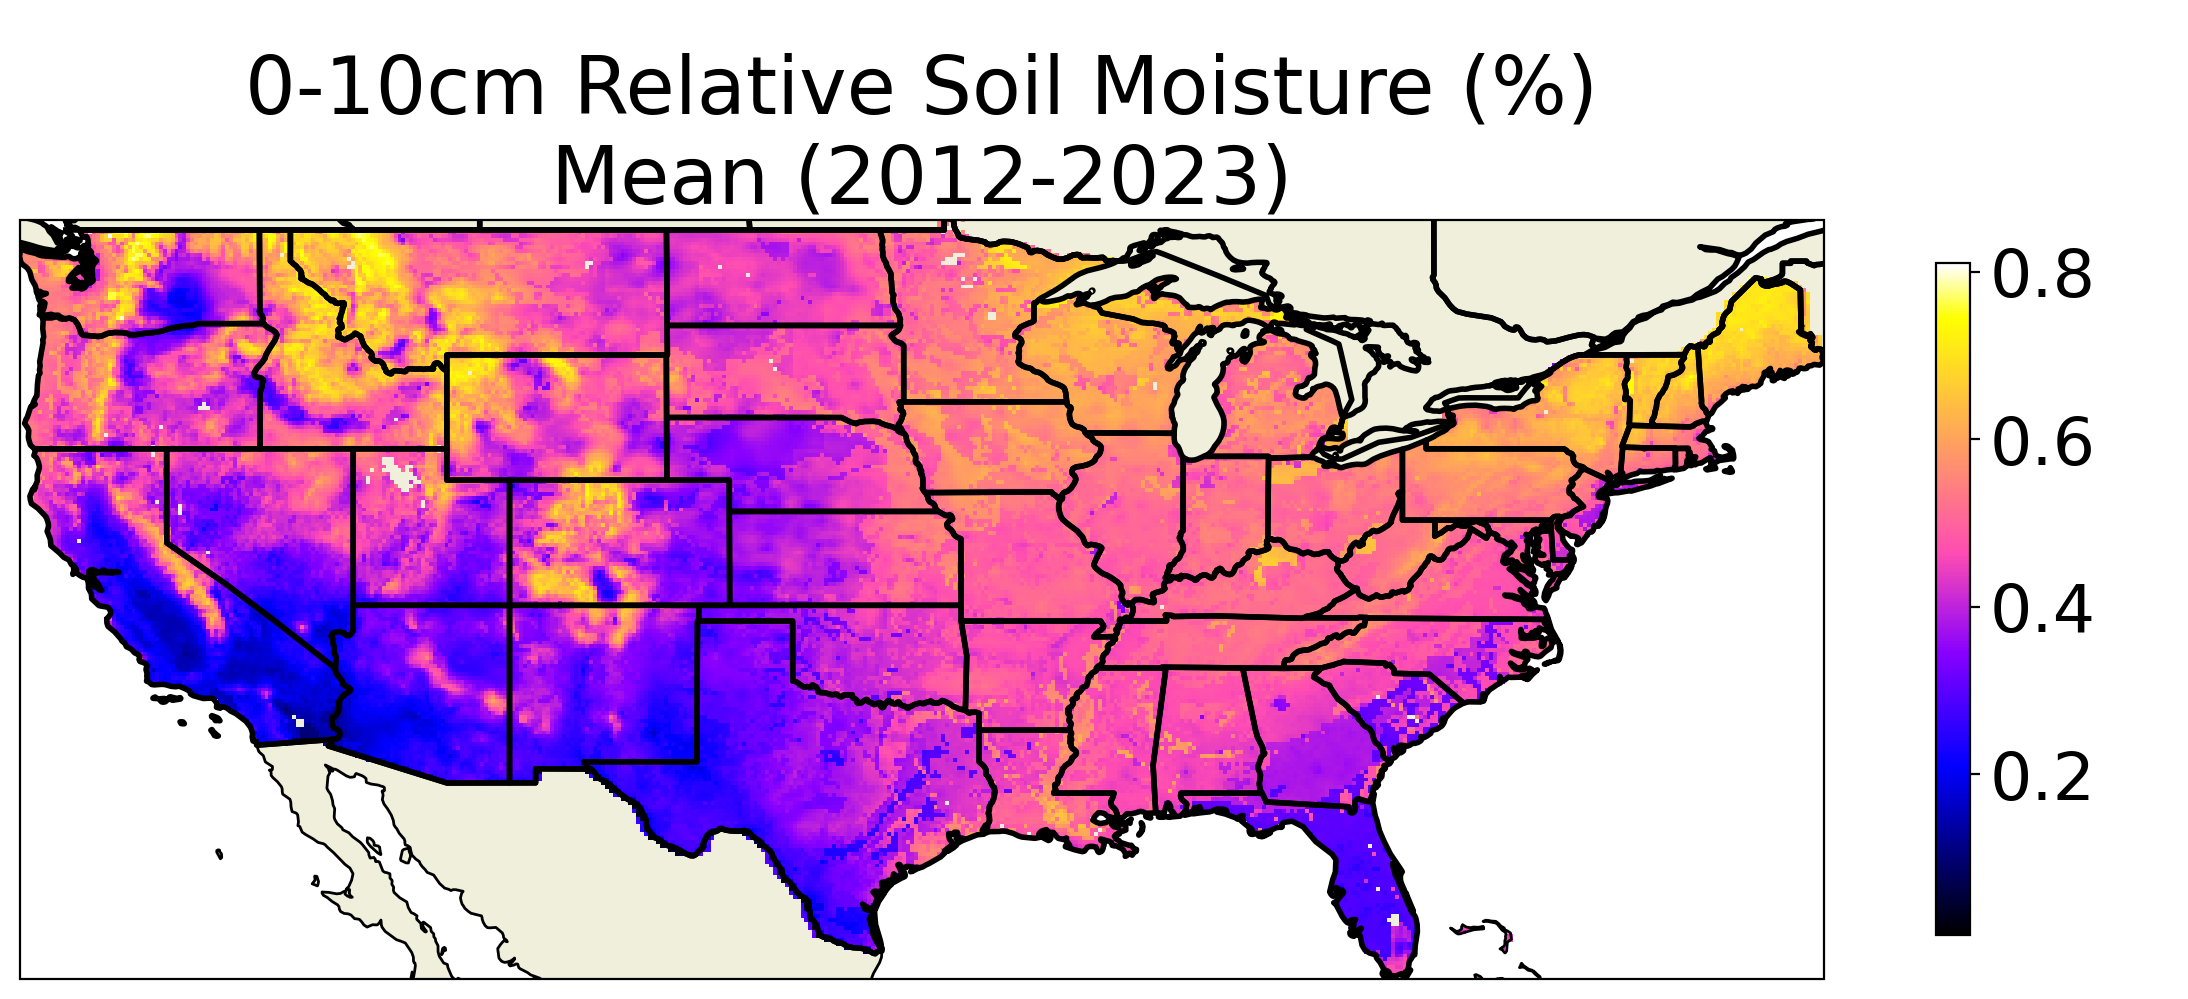
\includegraphics[width=.48\linewidth]{figures/thesis-gridstats/gridstat-bulk_rsm-10_2012-1_2023-12_y000-195_x000-462_mean.png}
    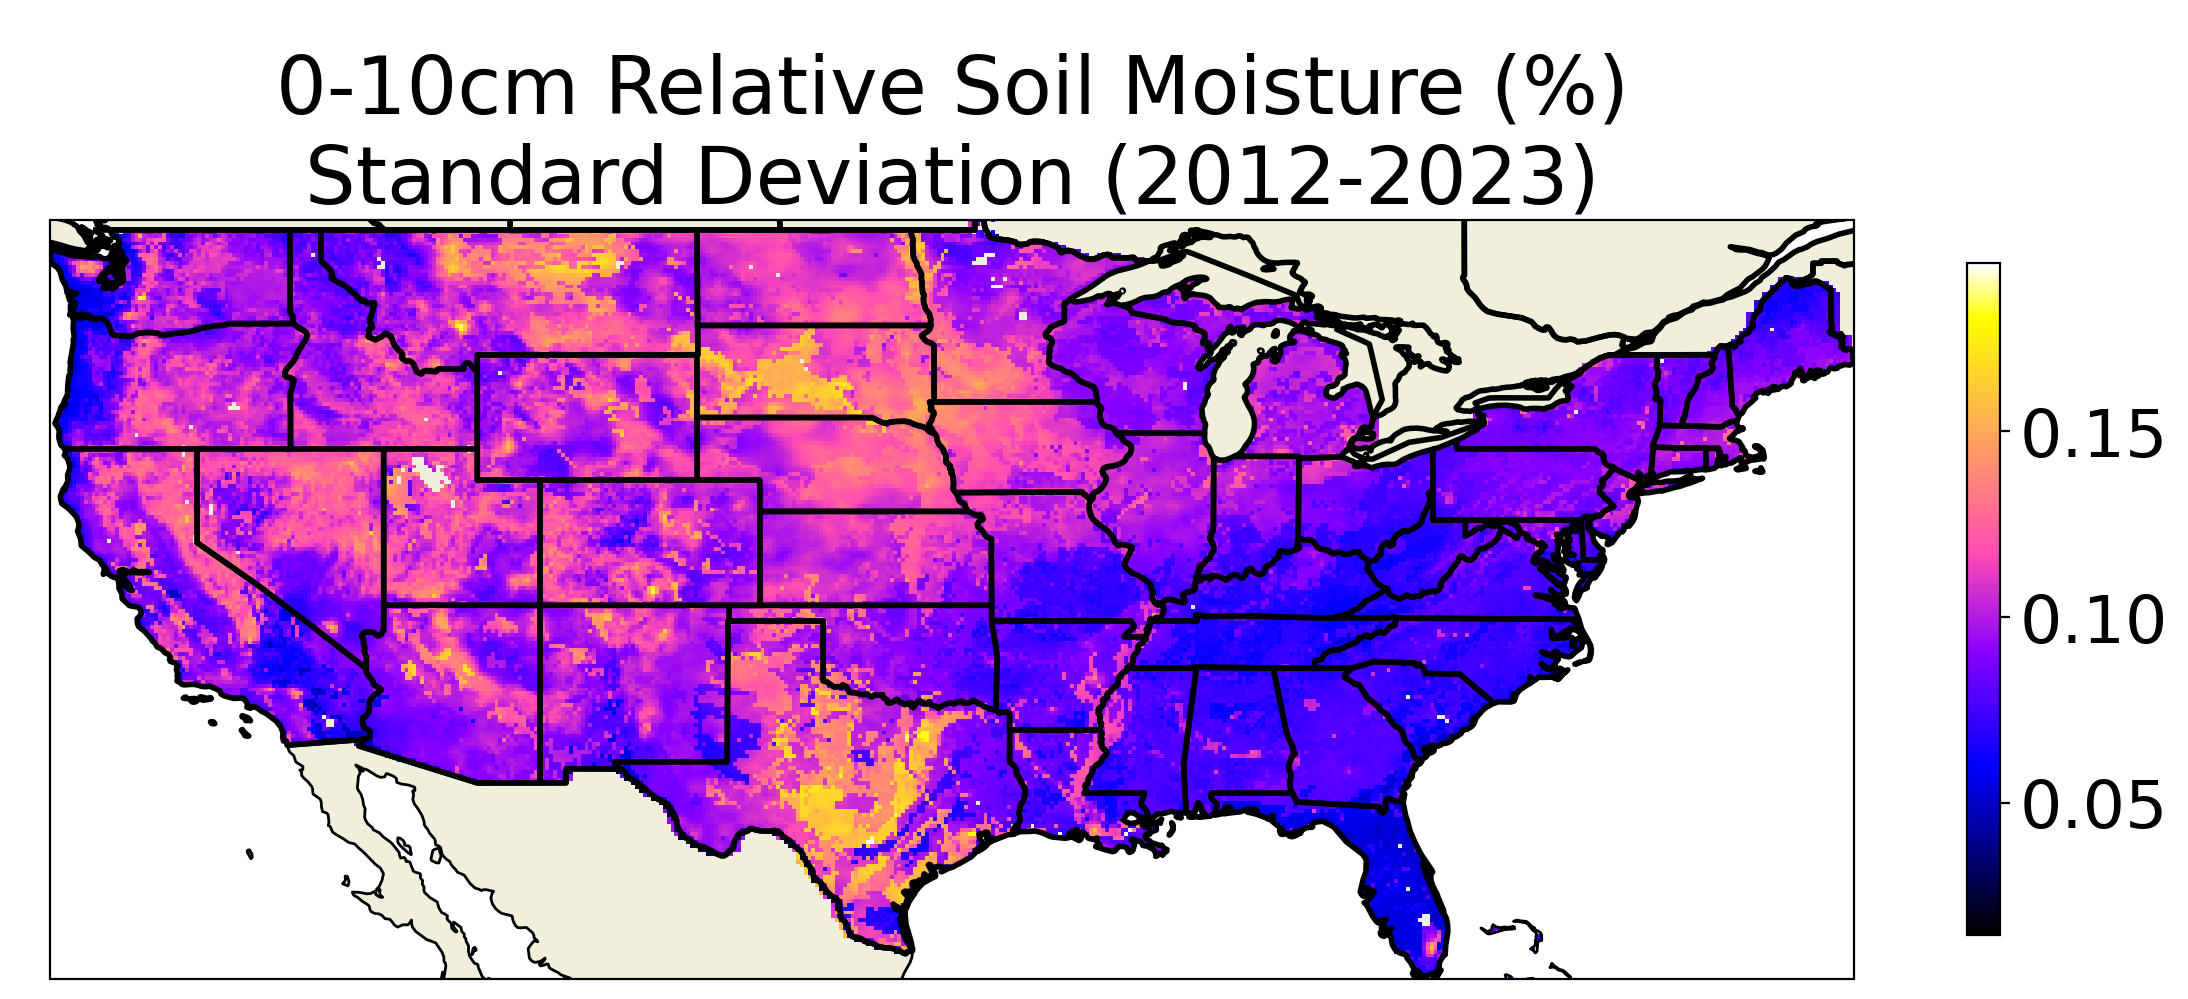
\includegraphics[width=.48\linewidth]{figures/thesis-gridstats/gridstat-bulk_rsm-10_2012-1_2023-12_y000-195_x000-462_stdev.png}
    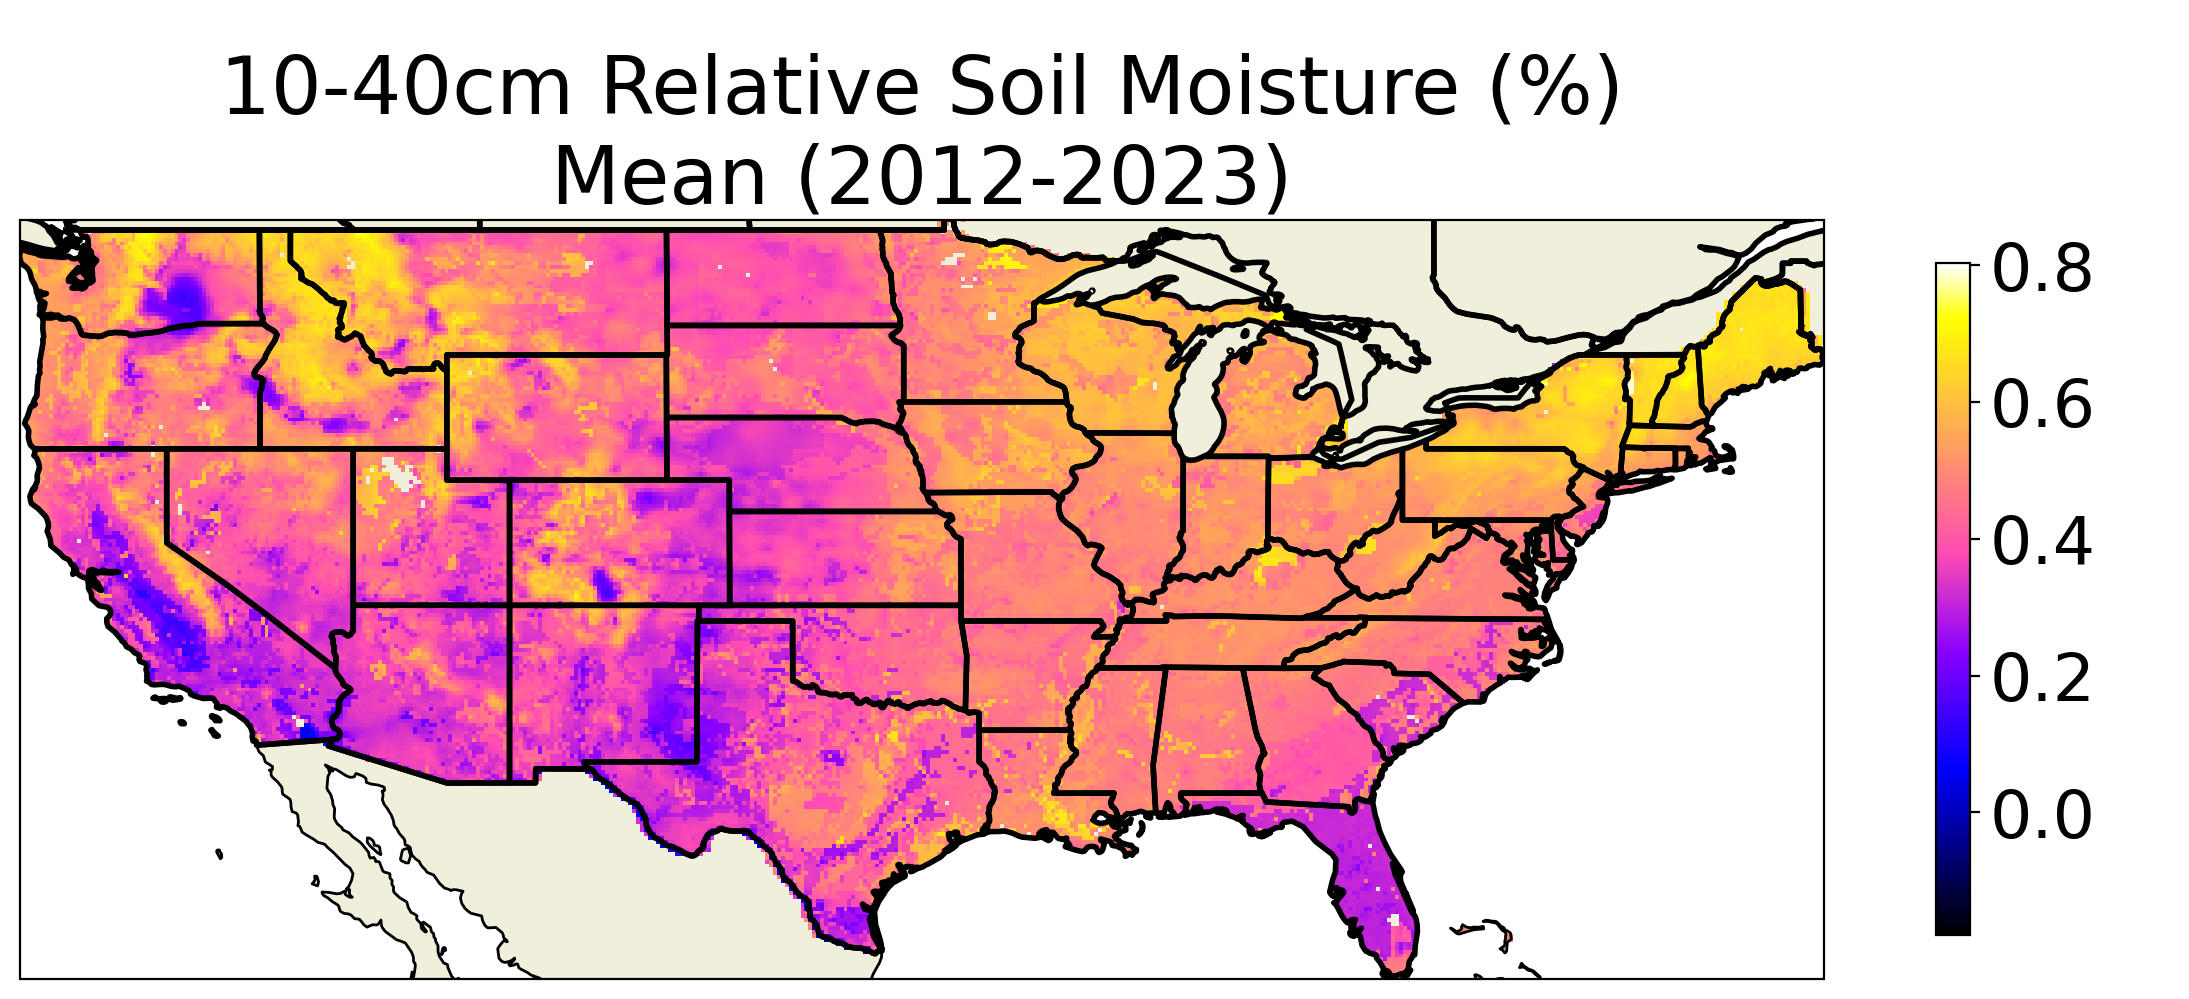
\includegraphics[width=.48\linewidth]{figures/thesis-gridstats/gridstat-bulk_rsm-40_2012-1_2023-12_y000-195_x000-462_mean.png}
    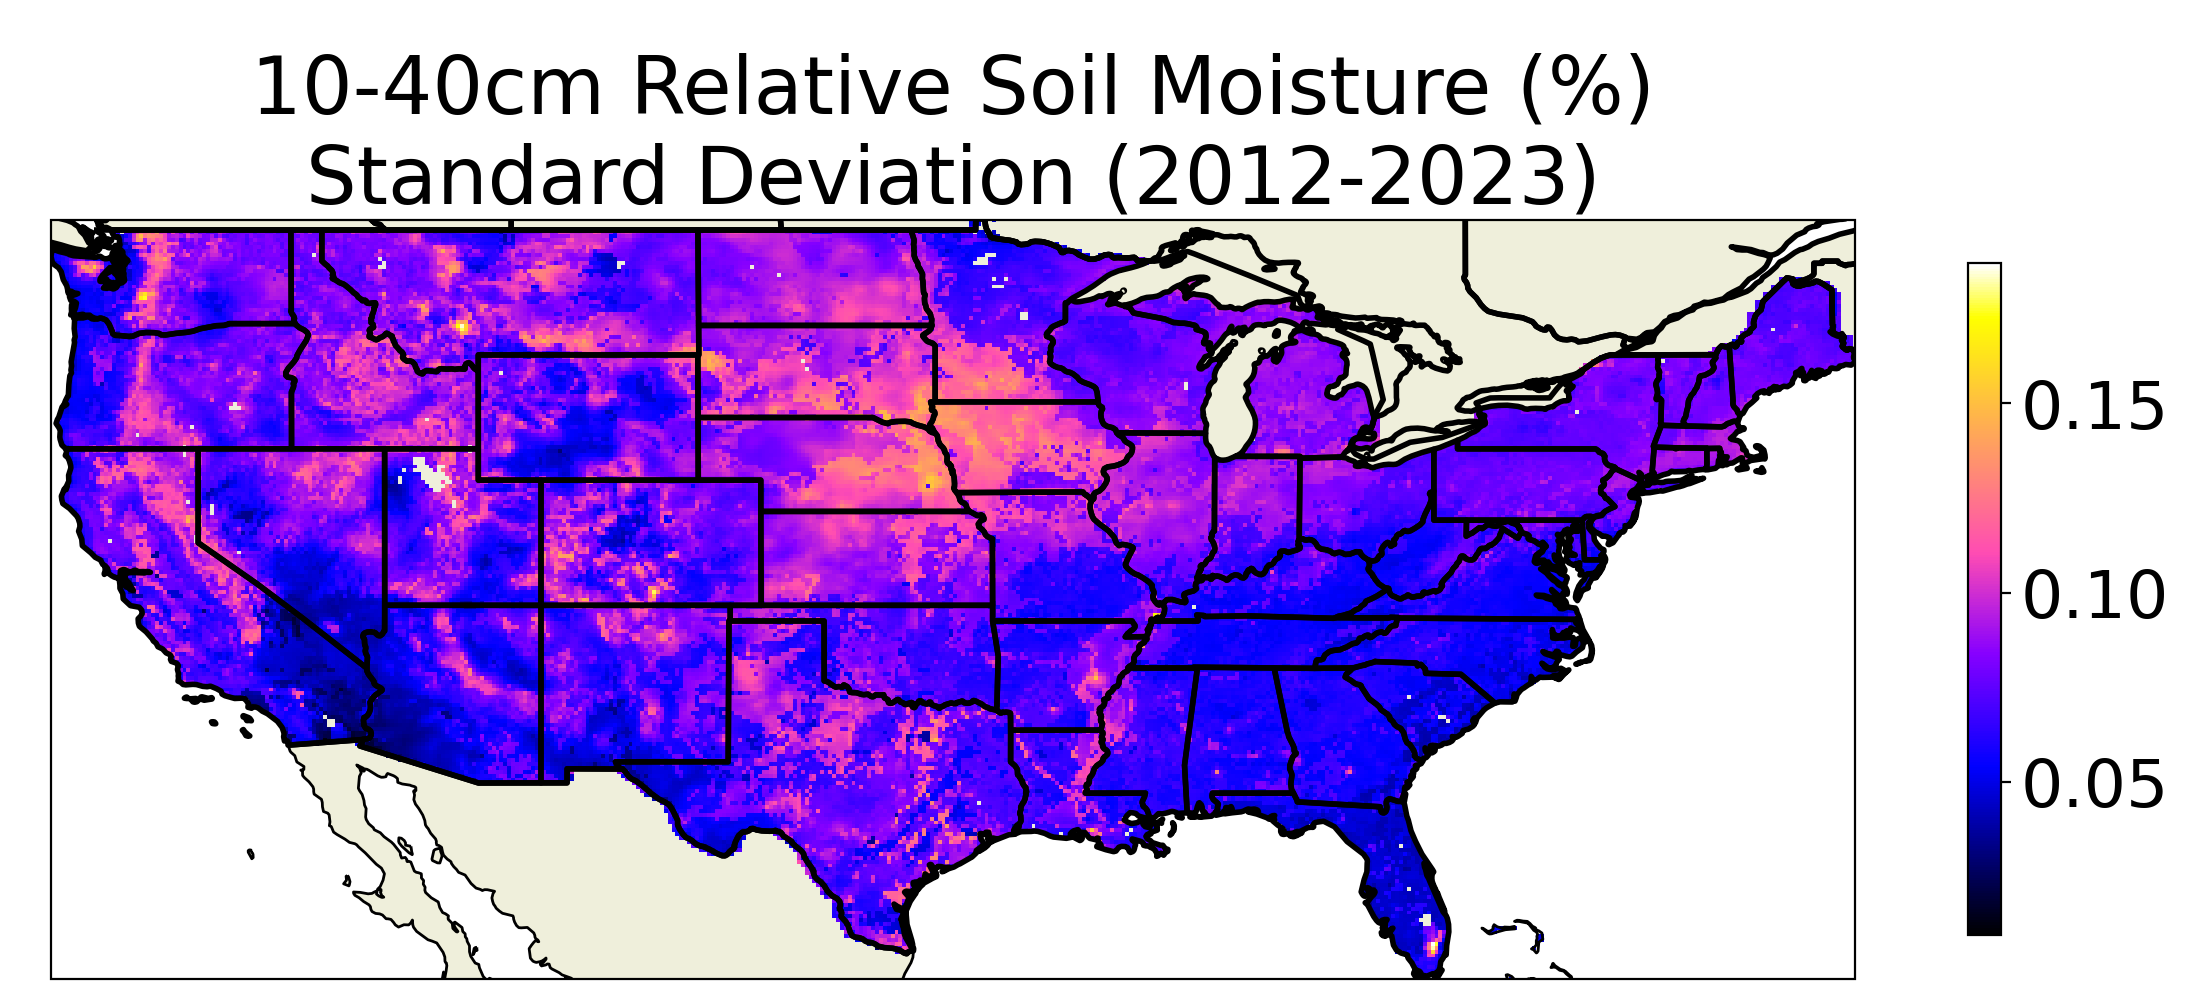
\includegraphics[width=.48\linewidth]{figures/thesis-gridstats/gridstat-bulk_rsm-40_2012-1_2023-12_y000-195_x000-462_stdev.png}
    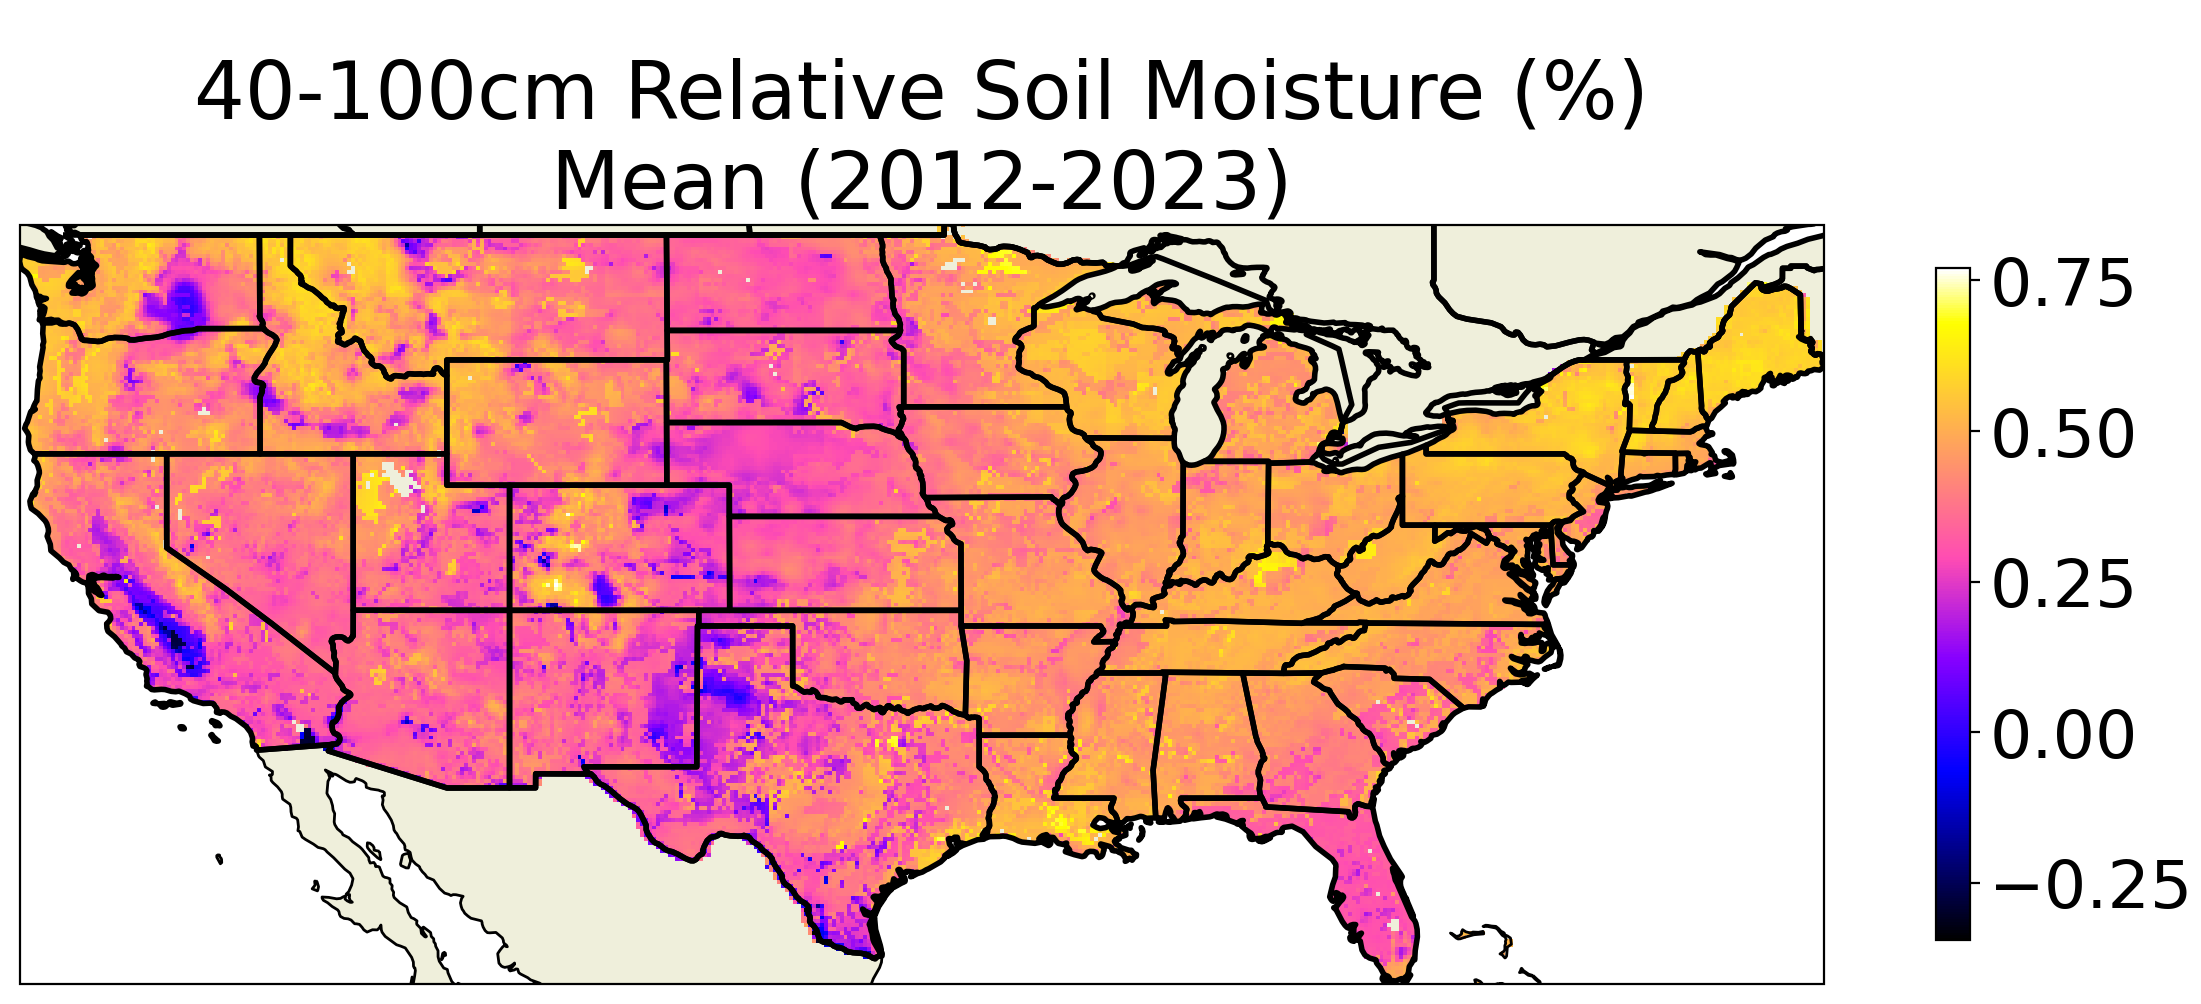
\includegraphics[width=.48\linewidth]{figures/thesis-gridstats/gridstat-bulk_rsm-100_2012-1_2023-12_y000-195_x000-462_mean.png}
    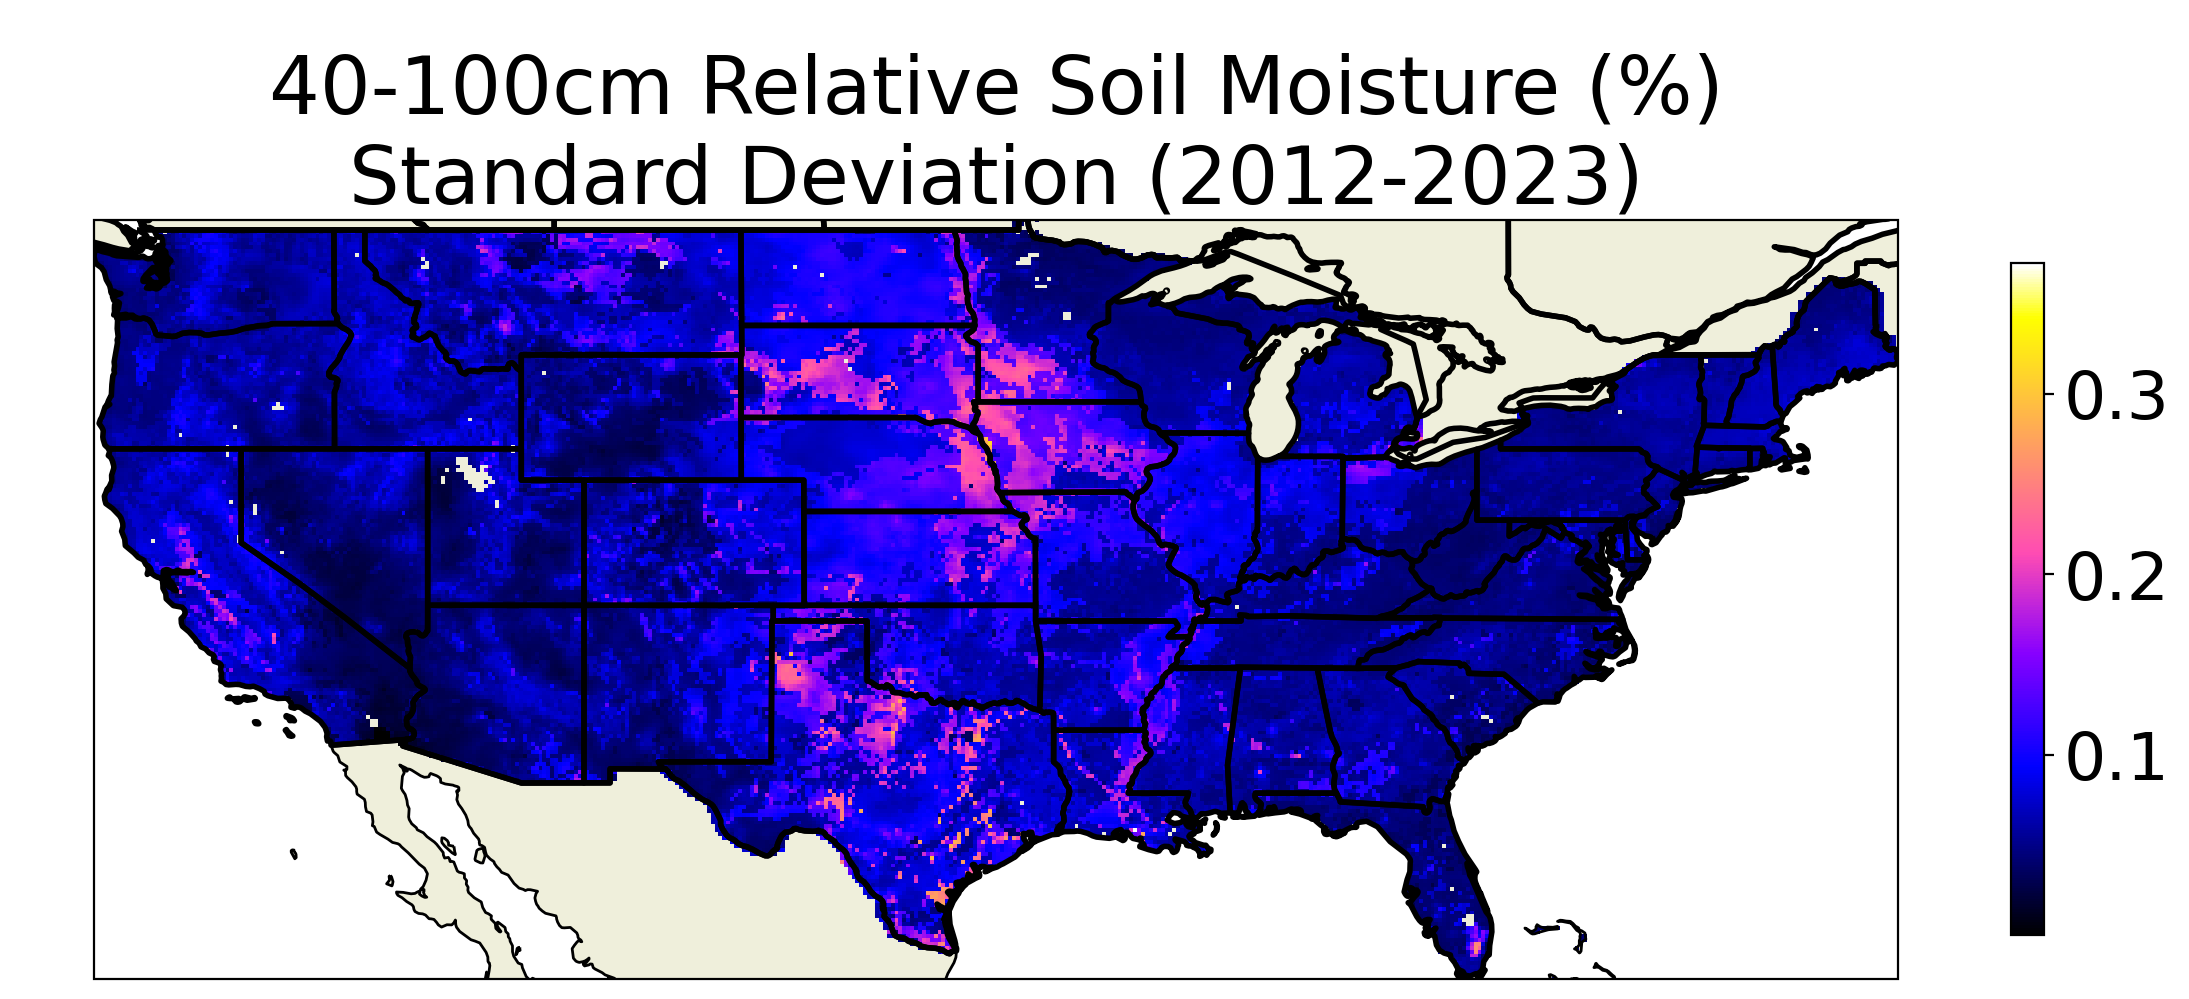
\includegraphics[width=.48\linewidth]{figures/thesis-gridstats/gridstat-bulk_rsm-100_2012-1_2023-12_y000-195_x000-462_stdev.png}
    \caption{Gridded mean and standard deviation of relative soil moisture (2012-2023)}
    \label{gs-rsm}
\end{figure}

The spatial variation of soil moisture is depicted in Figure \ref{dist-soilm}, which emphasizes several important regional distinctions. The mountainous regions of the West remain rather saturated for much of the year -- especially in the upper soil layers -- owing to their high precipitation rates, the consistent presence of a snow pack, and limited drainage due to frozen soil.

\section{Model Architectures}

The models that we tested fall into 3 broad architectural categories, as outlined in the background: fully-connected neural networks (FNNs), na\"ive RNNs, and LSTMs. In this subsection, we will elaborate on the particular implementation of these

\begin{figure}[h!]
    \centering
    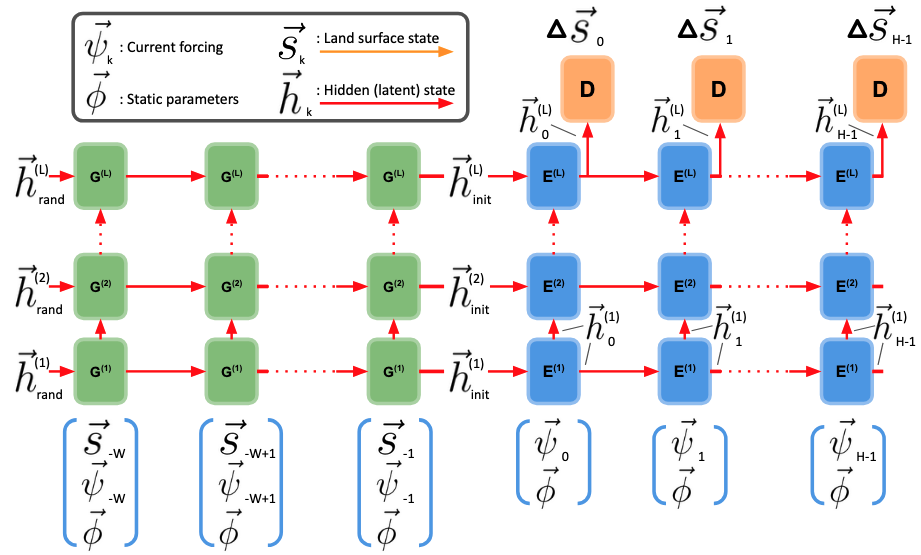
\includegraphics[width=.95\linewidth]{figures/schematic_s2s-default.png}

    \caption{Sequence-to-sequence RNN architecture with spin-up window cells \textbf{G} for initializing first-step weights, and fully-connected decoder \textbf{D}.}
    \label{s2s-default}
\end{figure}

The spin-up window layers prior to the first timestep (\textbf{G}$^{(s)}$ in Figure \ref{s2s-default}) have their own sets of weights since the first-layer arguments include the known past soil states. Only the hidden states corresponding to the final timestep are captured from each layer of the spin-up window, and are exclusively used to provide historical information to the initial timesteps of the corresponding layers in the prediction horizon sequence. The accumulation step for calculating the new state $\vec{s}_{k+1}$ with the decoded prediction of increment change in state also emphasizes another property of ANN-based models: unlike numerical models akin to the dynamical system described by Equation \ref{dynamical}, the ANNs abstract away the concept of a variable increment time between prediction steps. Instead, the ANNs are trained to make predictions at a fixed timestep that cannot be changed during inference.

\begin{figure}[h!]
    \centering
    \includegraphics[width=.95\linewidth]{figures/schematic_s2s-accumulator.png}

    \caption{Sequence-to-sequence RNN with explicit output state accumulation.}
    \label{s2s-default}
\end{figure}

\section{Training Paradigm}

\begin{figure}[h!]
    \centering
    \includegraphics[width=.48\linewidth]{figures/cyclical_lr_logarithmic.png}
    \includegraphics[width=.48\linewidth]{figures/learning-curves_acclstm.png}

    \caption{Sequence-to-sequence RNN with explicit output state accumulation.}
    \label{learning-rate}
\end{figure}

\section{Evaluation System}

